\chapter{Estratégias de Combate ao Problema}\label{ch:Relacionados}


O Abuso Sexual Infantil (ASI) manifesta-se como um problema global. Diante disso, profissionais da saúde e pesquisadores passaram a se dedicar a compreender as raízes  deste mal que assola milhares de crianças todos os anos \cite{deslandes1994atenccao, dahlberg2006violencia, da2017violencia}. A área de criminologia em específico, desenvolveu uma série de teorias acerca das causas para os atos infracionais. Dentre elas, destaca-se a Teoria da Atividade Rotineira, ilustrada na \autoref{fig:Crime}.
%Inúmeros métodos surgiram para compreender as raízes do problema, dentre eles, cita-se a Análise de Causa Raiz (ACR). Tal método visa descobrir a causa de um problema para identificar soluções adequadas \cite{rooney2004root}.

\begin{wrapfigure}{r}{7.1cm}
  \caption{\label{fig:Crime}Triângulo do Crime.}
      \begin{center}
        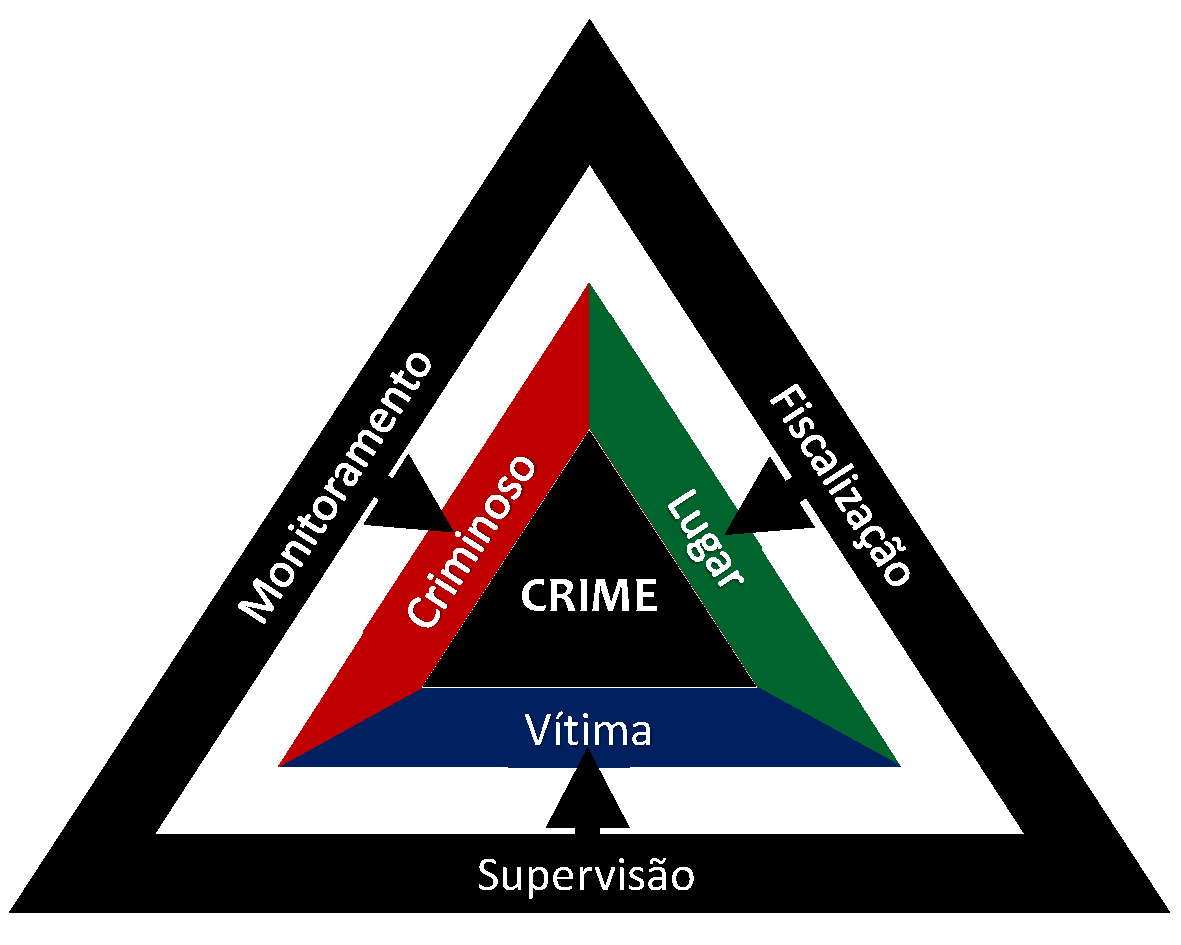
\includegraphics[width=\linewidth]{./Figuras/TrianguloCrime.pdf}
      \end{center}
      \legend{Fonte: Os autores (2020)}
\end{wrapfigure}

O infográfico da \autoref{fig:Crime} apresenta os três elementos básicos da Teoria da Atividade Rotineira, também conhecida como Triângulo do Crime. Em resumo, três elementos são considerados essenciais para a ocorrência de um crime. Para que um crime aconteça deve-se haver um criminoso motivado sem supervisão, um lugar sem fiscalização e uma vítima desprotegida ou vulnerável. Tomar atitudes preventivas sob qualquer um destes elementos, dificulta a ocorrência do crime. Todavia, destaca-se que estes elementos não possuem pesos iguais, mas sim, se interbalanceiam entre si (e.g. em certas condições, um lugar bem fiscalizado poderia não ser um empecilho para um criminoso muito motivado).



%criminoso = supervisão
%lugar = fiscalização
%Vítima = proteção

O Triângulo do Crime apresenta as três partes fundamentais para a ocorrência de um crime. As estratégias de combate ao abuso sexual infantil se objetivam a agir sob estas partes fundamentais. Algumas estratégias são focadas no monitoramento de criminosos\footnote{\label{note:nota1}Círculos de Suporte e Responsabilidade (Em inglês: Circles of Accountability and Support - CoSA) são grupos de voluntários com supervisão profissional para apoiar os agressores sexuais à medida que se reintegram à sociedade após serem libertados do encarceramento.}, outras no fortalecimento da fiscalização de espaços públicos ou privados\footnote{Lei nº 12.038, de 1º de outubro de 2009 dificulta a exploração sexual de crianças e adolescentes impossibilitando a hospedagem deles por terceiros que não apresentem autorizações legais.}, e outras na capacitação preventiva de potenciais vítimas, tornando-as menos vulneráveis\footnote{O programa educacional Talking about Touching é um programa focado no ensino de habilidades básicas para crianças com finalidade de ajudá-las a se protegerem de situações abusivas.}. Cada estratégia pode ser dividida com base em seus níveis de prevenção. Os níveis de prevenção são apresentados em maiores detalhes na \autoref{fig:prevencao}.

\begin{figure}[htb]
	\caption{\label{fig:prevencao}Níveis de Prevenção.}
  \begin{center}
    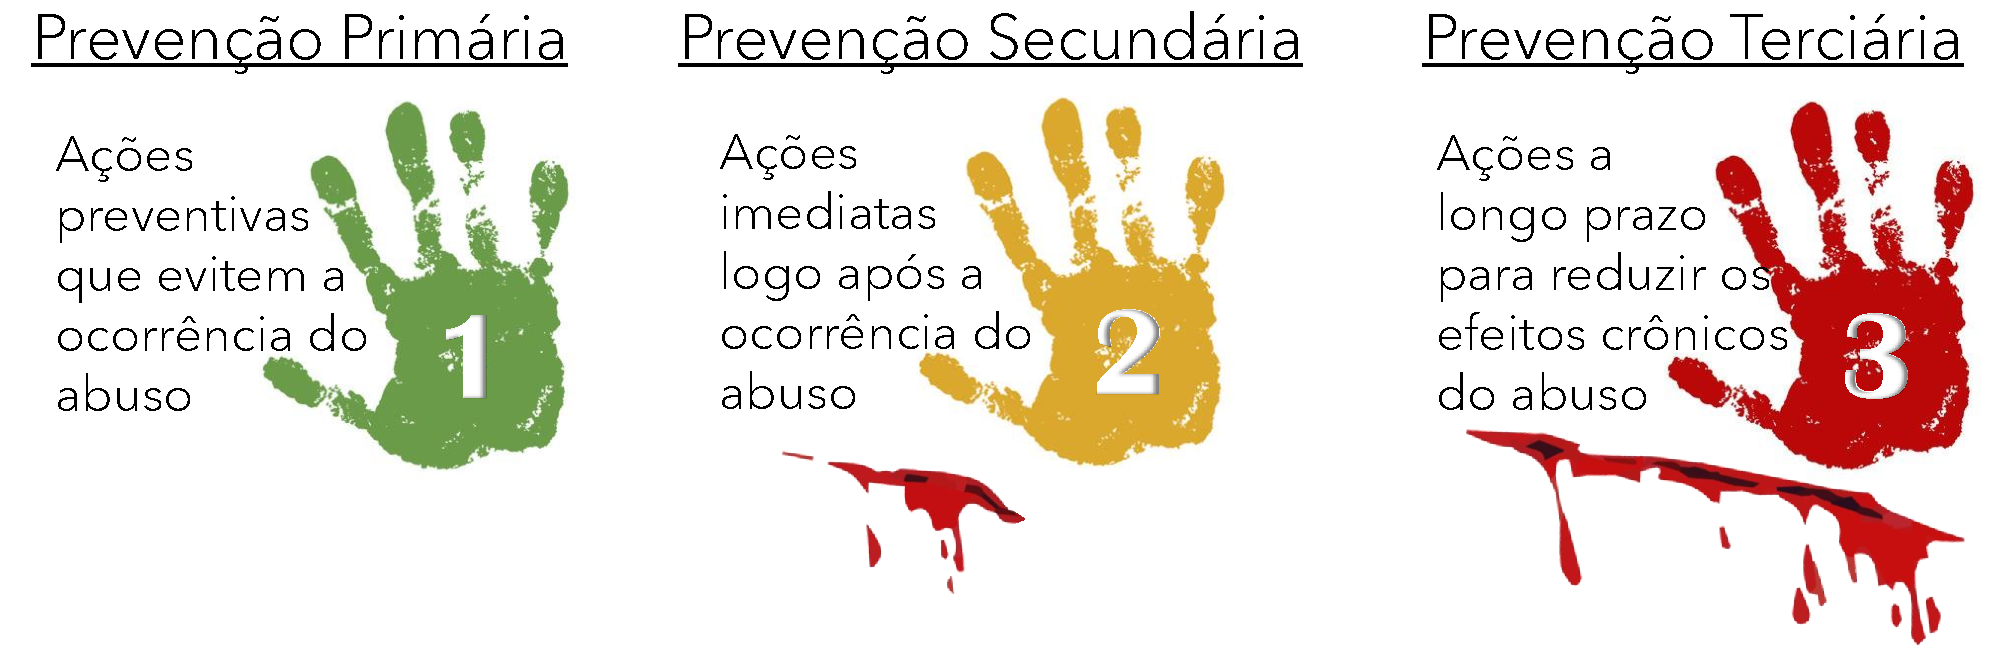
\includegraphics[width=\linewidth]{./Figuras/Prevencao.pdf}
	\end{center}
	\legend{Fonte: Os autores (2020)}
\end{figure}

A \autoref{fig:prevencao} apresenta os três níveis de prevenção mais comumente relatados na literatura pesquisada. São eles: prevenção primária, prevenção secundária e prevenção terciária \cite{dahlberg2006violencia, santos2011guia, maria2012abusos}. No caso do abuso sexual infantil, a prevenção primária engloba iniciativas que antecipam a incidência do abuso sexual contra crianças e adolescentes  \cite{marcelino2017vamos}. A prevenção secundária enfatiza uma resposta imediata após a ocorrência da violência sexual. Já a prevenção terciária corresponde, de modo geral, a ações de longo prazo para o tratamento e recuperação das vítimas \cite{people2020expert}. Informa-se que a literatura médica relata também um quarto nível de prevenção. A prevenção quaternária descreve sobre ações preventivas contra eventuais exageros na utilização de métodos preventivos \cite{tesser2017importante}. Embora presente na literatura médica, salienta-se que a atual dissertação engloba apenas os três níveis de prevenção mais relatados pela bibliografia pesquisada acerca do abuso sexual infantil.

Os níveis de prevenção do abuso sexual infantil não se resumem a atuar apenas sob as crianças. Há registros de prevenção terciária relacionados inclusive ao tratamento/acompanhamento de agressores sexuais\footref{note:nota1}. O combate ao abuso sexual infantil assume então inúmeras facetas, cada qual, objetivada a diminuir de alguma forma os fatores de risco que influenciam a ocorrência de violações sexuais.

Os Fatores de Risco são aquelas circunstâncias que aumentam a probabilidade da ocorrência de um episódio de violência. Deste modo, o abuso infantil apresenta mais chances de ocorrer quando os fatores de risco se acumulam. Os Fatores de Risco interagem entre si, no que é chamado de risco em cascata, no qual um risco inicial pode acompanhar ou desencadear outros riscos, terminando por resultar em um acúmulo sucessivo de fatores de risco \cite{Recommendations2019Taylor}. A \autoref{fig:Riscos} apresenta a disposição dos fatores de riscos mais apontados pela literatura na área por meio de um Modelo Ecológico. 

%O modelo socio-ecológico é uma estrutura de saúde pública desenvolvida pelos Centros de Controle e Prevenção de Doenças (em inglês: Centers for Disease Control and Prevention - CDC) \cite{centers2019social}. O modelo socio-ecológico data desde a década de 1970, sendo  aplicado aos casos de abuso infantil \cite{dahlberg2006violencia}. O modelo explora a relação entre os fatores individuais e contextuais e considera a violência como produto dos múltiplos níveis de influência sobre o comportamento


%https://www.scielo.br/pdf/csc/v11s0/a07v11s0.pdf \cite{dahlberg2006violencia}

%https://www.unicef.org/media/66741/file/Promising-programme-responses.pdf4 \cite{topromising}

%https://www.k12.wa.us/sites/default/files/public/hivsexualhealth/pubdocs/Erin%27s%20Law%20Report.pdf [fez que nem eu] \cite{Recommendations2019Taylor}

%https://www.doh.wa.gov/Portals/1/Documents/Pubs/140-165-SexualViolencePreventionPlan.pdf [fez que nem eu] \cite{sexual2017department}

%https://www.cdc.gov/violenceprevention/pdf/svprevention-a.pdf \cite{centers2004sexual}

\begin{figure}[htb]

	\caption{\label{fig:Riscos}Modelo Ecológico.}
  \begin{center}
    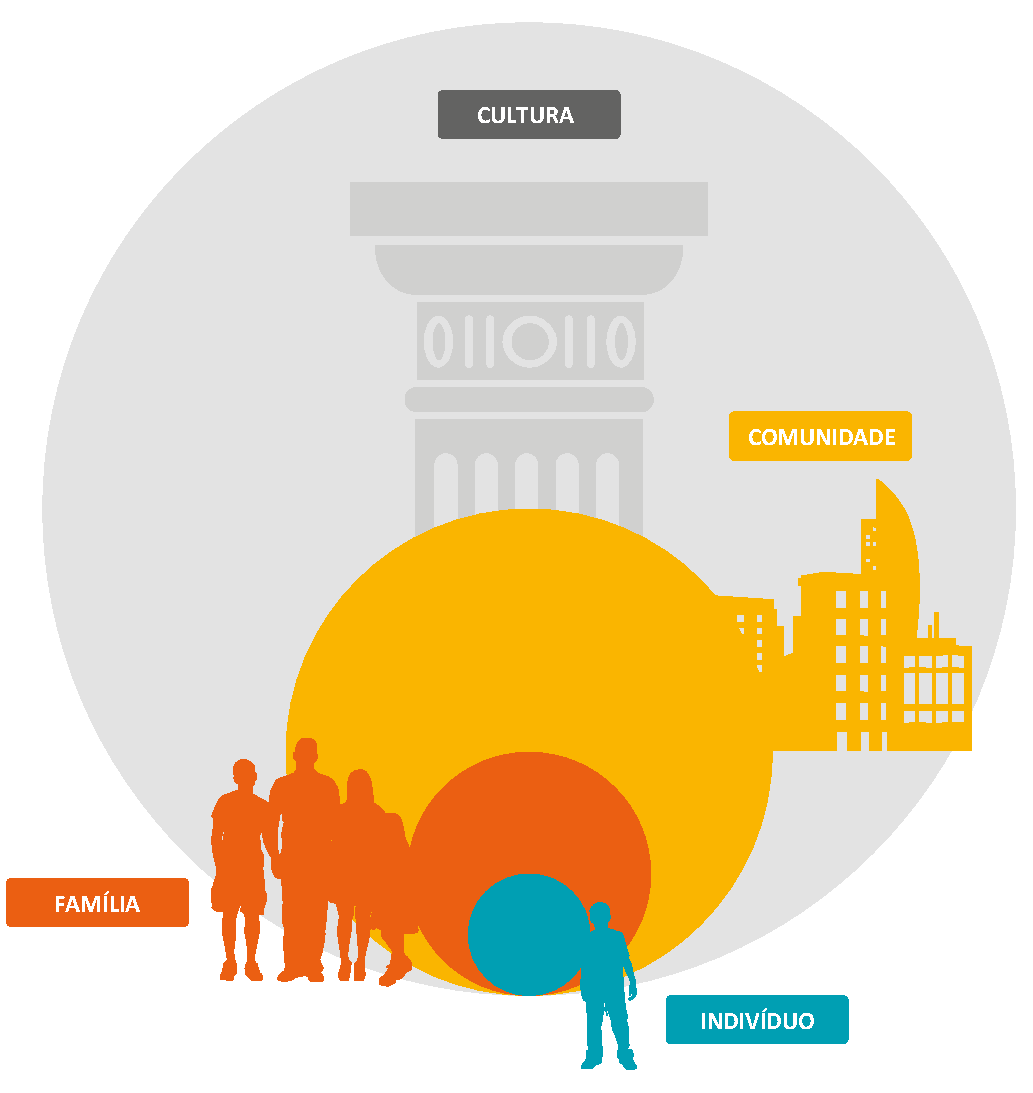
\includegraphics[width=0.75\linewidth]{./Figuras/FatoresRisco.pdf}
	\end{center}
  \legend{Fonte: adaptado de \citeonline[p. 20]{blasco2018abuso}.}

\end{figure}
%https://www.savethechildren.es/sites/default/files/imce/docs/mas_me_duele_a_mi.pdf
%[ainda sita-se a falta de sensibilização da sociedade, lideres politicos, etc tec.... pag 39]

O Modelo Ecológico da \autoref{fig:Riscos} ilustra os quatro fatores de risco mais presentes na bibliografia pesquisa. Salienta-se que os fatores de risco podem variar em quantidade e em nomenclatura, dependendo da fonte literária \cite{centers2004sexual, sexual2017department, blasco2018abuso, topromising}. Todavia, a ideia base do Modelo Ecológico tende a permanecer inalterada. O modelo em si, explora a relação entre os fatores individuais e contextuais que acabam por implicar em um cenário de violência \cite{dahlberg2006violencia}. Os fatores de risco do abuso sexual infantil mais influentes são:

\begin{itemize}
  \item \textbf{Indivíduo:} \hfill Aspectos individuais que fomentem a ocorrência do abuso sexual. %Válido tanto para as vítimas quanto para os agressores. 
  \item \textbf{Família:} \hfill Questões familiares que viabilizam as condições para a violência.  %circunstâncias
  \item \textbf{Comunidade:} Condições econômicas e governamentais que propiciem o abuso.
  \item \textbf{Cultura:} \hfill Crenças sociais que estimulem atividades sexuais com menores. 
\end{itemize}


Os fatores de risco podem interatuar entre si de modo a maximizar as chances de um evento abusivo. O baixo nível educacional de um \textbf{Indivíduo} é um dos elementos a ser citado neste aspecto \cite{dahlberg2006violencia}. A negligência da \textbf{Família} nos cuidados infantis é outro aspecto a ser citado \cite{blasco2018abuso}. Cita-se também, a permissividade do casamento infantil de algumas \textbf{Culturas} \cite{bandiera2017women}. Assim, como a baixa condição socioeconômica de uma \textbf{Comunidade}. A exemplo, soros positivos de comunidades africanas veem o relacionamento sexual com crianças como um ato de limpeza e cura da síndrome da imunodeficiência adquirida \cite{aded2006abuso}.

%Na Africa, ``as crianças correm grande risco de contaminação pelo vírus HIV''.. existe a crença que os portadores serão limpados da doença. \cite{aded2006abuso} [possivelmente falar sobre isso na hora de falar do treinamento para os pais]

%``We evaluate a \textbf{multifaceted policy intervention} attempting to jumpstart adolescent women’s empowerment in Uganda'' ... ``Strikingly, the share of girls reporting sex against their will drops by close to a third and aspired ages at which to marry and start childbearing move forward.'' \cite{bandiera2017women} [BRAC-ELA as a tool to aid womens’ empowerment]

Agir sobre os fatores de risco (\autoref{fig:Riscos}), implica em agir de forma mais efetiva no combate a violência sexual infantil. Compreender os níveis de prevenção (\autoref{fig:prevencao}), implica em compreender os momentos de atuar sobre o problema. Entender as raízes da violência (\autoref{fig:Crime}), implica em entender seus elementos operantes. Estudar o problema do abuso sexual infantil, é necessário para se ter um panorama geral acerca dos possíveis cenários de atuação e combate. Além disso, um levantamento bibliográfico sobre as estratégias de combate já desenvolvidas se faz indispensável para evitar a perda de tempo e dinheiro no desenvolvimento de uma solução já existente \cite{wazlawick2014metodologia}. 

Este Capítulo elenca as principais soluções utilizadas no combate ao abuso sexual infantil de acordo com a bibliografia pesquisada. O levantamento bibliográfico fundamenta-se nos seguintes mecanismos de busca acadêmica (MBAs): ACM DL, IEEExplore, Science Direct e Web of Science. A escolha por esses MBAs deu-se por abrigarem publicações de qualidade reconhecida pela Coordenação de Aperfeiçoamento de Pessoal de Nível Superior (CAPES) \cite{capes2016}%e por possuírem a maior quantidade de recursos de busca e seleção \cite{buchinger2014mecanismos}
. Também foram pesquisados periódicos, livros, revistas científicas e \textit{sites} de referência na área; além de consultadas as citações referenciadas nesta dissertação. 

Diante do exposto, a presente dissertação divide as Seções deste Capítulo em grupos de soluções utilizadas no combate ao abuso sexual infantil. Cada solução visa mitigar o problema da sua própria maneira. Dentre as soluções apresentadas, informa-se que as soluções baseadas em jogos são abordadas mais profundamente em relação as demais, por se tratarem do cerne da atual pesquisa. Dito isso, a \autoref{sec:regras} descreve normas e legislações sobre os direitos das crianças, a \autoref{sec:canais} apresenta algumas formas de denúncia, a \autoref{sec:propagandas} aponta ações publicitárias, a \autoref{sec:hospital} trata de questões hospitalares, a \autoref{sec:centros} apresenta os centros de atendimento, a \autoref{sec:dp} lista algumas delegacias especializadas, a \autoref{sec:op} elenca operações policiais, a \autoref{sec:infratores} apresenta alguns tratamentos com infratores, a \autoref{sec:programas} menciona alguns programas de capacitação, a \autoref{sec:materiais} relata materiais didáticos de ensino e a \autoref{sec:finais} dá as considerações finais do presente Capítulo. 

%\autoref{ssec:pais}
%\autoref{ssec:professores}
%\autoref{ssec:alunos}

%\autoref{ssec:analogico}
%\autoref{ssec:digitais}
%\autoref{ssec:jogos}




%procurando aumentar o conhecimento dos menores na problemática em questão, tornando-as mais resilientes e menos vulneráveis

%, visando mitigar os males iniciais causados por um evento de abuso

%https://repositorio.ufscar.br/bitstream/handle/ufscar/2835/TeseMGSP.pdf?sequence=1&isAllowed=y

%https://www.udesc.br/arquivos/cct/id_cpmenu/1024/disserta_ao_completa_15532596804969_1024.pdf

%https://www.scielo.br/pdf/csc/v11s0/a07v11s0.pdf

%http://portaldoprofessor.mec.gov.br/storage/materiais/0000016936.pdf

%https://www.scielosp.org/article/csc/1999.v4n1/171-181/pt/

%https://repositorio.iscte-iul.pt/bitstream/10071/15660/1/Disserta%c3%a7%c3%a3oDianaMarcelino.pdf

%https://repositorio.iscte-iul.pt/bitstream/10071/12615/3/2016_ECSH_DPSO_Dissertacao_Magda%20Moita.pdf

%https://repositorio.iscte-iul.pt/bitstream/10071/10673/1/2015_ECSH_DPSO_Dissertcao_Nicole%20Christine%20Alves%20Figueiredo.pdf

%https://www.unicef.org/media/66741/file/Promising-programme-responses.pdf4

%http://repositorio.ispa.pt/bitstream/10400.12/1768/1/TES%20MARI1.pdf

%https://www.k12.wa.us/sites/default/files/public/hivsexualhealth/pubdocs/Erin%27s%20Law%20Report.pdf

%https://www.cdc.gov/violenceprevention/pdf/svprevention-a.pdf

%https://www.doh.wa.gov/Portals/1/Documents/Pubs/140-165-SexualViolencePreventionPlan.pdf

%https://bmcpublichealth.biomedcentral.com/articles/10.1186/s12889-017-4502-6

%https://www.gov.scot/publications/expert-group-preventing-sexual-offending-involving-children-young-people-prevention-responses-harmful-sexual-behaviour-children-young-people/pages/11/

%https://www.e-publicacoes.uerj.br/index.php/sustinere/article/view/30004/23155

%https://www.scielosp.org/article/csc/2006.v11suppl0/1163-1178/pt/

%https://endsexualviolencect.org/what-we-do/prevention/primary-prevention/

%e discutir medidas para sua prevenção


%\cite{eck1995examining}

%``Na década de 1980, profissionais da saúde como médicos, pesquisadores e os sistemas de  saúde  pública  passaram  a  se  dedicar  a  compreender  as  raízes  daviolência  e  discutir medidas   para   sua   prevenção.   É   também   nessa   década   que   a   violência   passa   a   ser considerada  um  problema  de  saúde  pública,  devido  ao  aumento  de  mortes  e  traumas  que congestionam os serviços de saúde (DESLANDES, 1994; DAHLBERG e KRUG, 2007).'' %https://www.e-publicacoes.uerj.br/index.php/sustinere/article/view/30004/23155


%\section{Teste $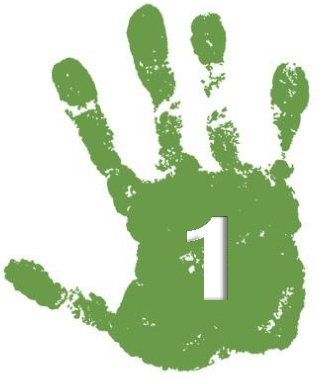
\includegraphics[width=0.05\linewidth]{./Figuras/Prevencao1.pdf}$$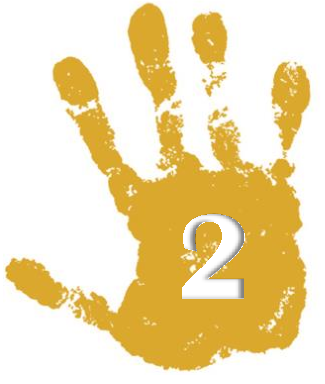
\includegraphics[width=0.05\linewidth]{./Figuras/Prevencao2.pdf}$$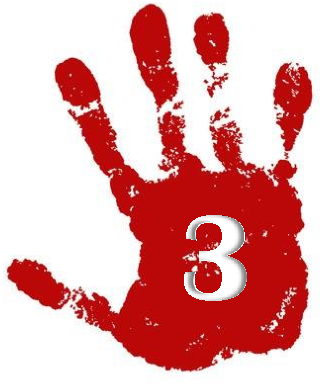
\includegraphics[width=0.05\linewidth]{./Figuras/Prevencao3.pdf}$}\label{sec:teste}%\icon{./Figuras/TrianguloCrime.pdf}


%Através dos escritos de Krafft-Ebing, o termo pedofilia foi criado no final do século XIX, quando a medicina por meio da psiquiatria começa a classificar os distúrbios mentais e os modos destoantes que deveriam ser banidos da sociedade. %https://www.riuni.unisul.br/bitstream/handle/12345/5994/tcc%20in%c3%a1cio%20-%20final.pdf?sequence=1&isAllowed=y

\section{Legislação}\label{sec:regras}%Normas, leis, regras, códigos

%O abuso sexual de crianças teve início na Antiguidade (desde 4 000 a.C.) e atualmente é um problema de saúde pública \cite{ribeiro2018programas}

%No Brasil, o período que antecedeu a Constituição Federal de 1988 (CF/88) foi determinantepara a mudança de paradigmas na área da garantia de direitos de crianças e adolescentes. A CF/88 foi um marco, na medida em que provocou uma substancial mudança no campo dos direitos humanos de crianças e adolescentes. O Brasil foi o primeiro país a promulgar um marco legal (Estatuto da Criança e do Adolescente), em consonância com a Convenção sobre os Direitos da Criança (1989). Estimase que o ECA tenha inspirado mais de 15 reformas legislativas, em especial na América Latina. %http://www.crianca.mppr.mp.br/arquivos/File/publi/sedh/08_2013_pnevsca.pdf 

%É dever constitucional da família, da sociedade e do Estado assegurar à criança e ao adolescente, com absoluta prioridade, o direito à vida, à saúde, à alimentação, à educação, ao lazer, à profissionalização, à cultura, à dignidade, ao respeito, à liberdade e à convivência familiar e comunitária. %https://www.riuni.unisul.br/bitstream/handle/12345/5994/tcc%20in%c3%a1cio%20-%20final.pdf?sequence=1&isAllowed=y

A elaboração de leis e normativas define um instrumento legal para a garantia dos direitos das crianças. Antes disso, no século XIX,
%A primeira monografia que descreve o abuso sexual infantil data de 1860 \cite{aded2006abuso}. Nesta época 
as cortes judiciais enxergavam os relatos de crianças que manifestavam o abuso sexual, como alegações fantasiosas ou mesmo mentirosas. A esperança das crianças de terem suas vozes devidamente ouvidas (e seus direitos assegurados) iria surgir apenas no século seguinte.
%https://bice.org/en/history-rights-child/
%https://childrightshub.org/en/history/

%“entre quase todos os povos antigos, tanto do Ocidente quanto do Oriente, os filhos durante a menoridade, não eram considerados sujeitos de direito, porém, servos da autoridade paterna.” (TAVARES apud OLIVEIRA, 2013).

%Mas, somente no final do século XIX, que a sociedade começou a mudar seu pensamento sobre a educação e tratamento destes indivíduos, o avanço era fraco, mas era um início, o surgimento da primeira concepção de criança. (OLIVEIRA, 2013).

No início do século XX, a sueca Ellen Key manifestou-se sobre o novo século denominando-o como `Século da Criança' \cite{sandin1999imagens, dos2015olhares, hayes2002children}. Este século marca a fundação da organização não governamental \textit{Save the Children}, responsável pela defesa dos direitos da criança no mundo. A fundação data de 1919, anos depois, em 1924 a fundadora da organização Eglantyne Jebb escreveu um documento que seria conhecido mundialmente como Declaração dos Direitos da Criança de Genebra ou Declaração de Genebra.

%http://www.un-documents.net/gdrc1924.htm [declaração de genebra]
%https://profuturo.education/en/2017/11/23/the-history-of-the-convention-of-the-rights-of-the-child/
A Declaração de Genebra estabelece cinco direitos fundamentais, os quais dão as crianças o direito de serem alimentadas, de serem ajudadas primeiro em caso de catástrofe, de serem escolarizadas, de serem bem tratadas e de serem protegidas contra qualquer forma de exploração. A Declaração dos Direitos da Criança de Genebra destaca-se na história como o primeiro documento internacional voltado a registrar e defender os direitos da criança. Em 1948 os direitos das crianças passaram a ser reconhecidos pela Declaração Universal dos Direitos Humanos, e pela Declaração dos Direitos da Criança adotada pela Assembleia Geral das Nações Unidas, em 1959 \cite{lelis2014fragmentaccao}. Anos depois em 1989, a Assembleia Geral da ONU adotou em suas normativas a Convenção sobre os Direitos da Criança, o qual tornou-se o instrumento de direitos humanos mais aceito na história, ratificado por 196 países. 
%http://www.revistas.usp.br/ran/article/view/124233/120991
%https://www.scielo.br/scielo.php?script=sci_arttext&pid=S0102-01881999000100002&lng=en&nrm=iso&tlng=pt
%https://www.scielo.br/pdf/rlae/v20n3/pt_a01v20n3.pdf
%http://www.publicadireito.com.br/artigos/?cod=99927ed3f11c0f36
%http://www.scj.pe.gov.br/scjpe/sites/all/themes/zentropy/pdf/producao_scj/CONSTRUINDOAERADOSDIREITOSHUMANOSporjoaocandido.pdf
%https://profuturo.education/en/2017/11/23/the-history-of-the-convention-of-the-rights-of-the-child/
%https://www.scielo.br/pdf/rpc/v33n4/a05v33n4.pdf
%https://www.tcd.ie/policy-institute/assets/pdf/BP9_Children_Hayes.pdf
%https://www.unicef.org/brazil/convencao-sobre-os-direitos-da-crianca

% Ano Internacional da Criança, em 1978

No Brasil, a história dos direitos das crianças e dos adolescentes começa em 1990, graças ao Estatuto da Criança e o Adolescente (ECA). O Estatuto é considerado um marco na defesa dos direitos da criança e do adolescente brasileiro \cite{lima2012direitos}. Os menores são protegidos pela legislação brasileira contra qualquer forma de negligência, discriminação, crueldade, opressão, violência e exploração. 

%Direito das crianças = 1924, pela Convenção de Genebra sobre os direitos da criança, estendida pela Convenção Internacional das Nações Unidas de 1959 e ratificada em 1990 pelos países signatários \cite{aded2006abuso} 

A legislação é um instrumento chave na luta contra o abuso sexual infantil. Os direitos estabelecidos juridicamente garantem uma maior proteção aos menores. A tipificação de crimes contra as crianças pode desencorajar certos agressores sexuais de praticarem seus delitos. Para os delitos já praticados, a legislação continua sendo um instrumento chave na luta contra o abuso sexual infantil, pois além de garantir tratamento as vítimas, assegura o encarceramento do criminoso sexual. Uma lei de 2014 por exemplo %(Lei 7220/14), 
torna hediondo o crime de exploração sexual de crianças e adolescentes, impedindo o condenado de obter anistia, graça ou indulto ou pagar fiança.

%Não falei sobre os códigos de conduta. 
%Não falei que a constituiçaõ de 1988 já estabelecia alguns direitos (e pelo que, algumas leis de anos anteriores também)
%https://books.google.com.br/books?hl=pt-BR&lr=&id=gHpmmREw-jwC&oi=fnd&pg=PA9&dq=conselho+tutelar&ots=csKHGcPPVh&sig=yxoM2HPB4x8ti8s9UU8EEkPOEBQ#v=onepage&q=conselho%20tutelar&f=false [capitulo 1 - evolução dos direitos]

\section{Ouvidorias e Canais de Denúncia}\label{sec:canais}

%``Foi criado o Disque-Denúncia Nacional de Abuso e Exploração Sexual Contra Crianças e Adolescentes – 0800-990500, sob a coordenação da Associação Brasileira Multidisciplinar de Proteção à Criança e ao Adolescente (Abrapia), através de convênio com oDepartamento da Criança e do Adolescente do Ministério da Justiça.''
%https://www.gov.br/mdh/pt-br/acesso-a-informacao/ouvidoria/Disque_Direitos_Humanos.pdf

%``O enfrentamento do violência sexual no âmbito dos \textbf{órgãos públicos estatais e federais ocorre em forma de campanhas de mobilização da cidadania}, através dos meios presentes de comunicação. Nas cidades, essas campanhas chegam através de chamadas, em emissoras de televisão, pela distribuição de panfletos e exposição de mensagens, de propagandas escritas, nas ruas, ou breves alertas nas emissoras de rádio. Também pela divulgação do \textbf{número telefônico 181} , que é reservado para denúncias dessa prática delitiva.'' ... ``enfrentamento da prática de abuso sexual que exige a presença de agentes vinculados ao Sistema Único de Assistência Social-SUAS, ao Sistema Único de Saúde-SUS, ao Sistema Nacional de Educação e às unidades locais de Segurança Pública'' [o artigo tambem falo do SIPIA-CT Web, CREAS e do CRAS] \cite{caccia2014conselheiros}

%O avanço da legislação trouxe ferramentas não só para combater e coibir esta violência, clareando o limite entre criança e adulto, mas para possibilitar a criação de medidas sócio-educativas, protetivas e preventivas frente aos danos psicológicos que muitas vezes podem ser irreversíveis, além dos efeitos físicos e sexuais. Nosso país foi o primeiro país a promulgar um marco legal com a criação do Estatuto da Criança e do Adolescente (ECA), \cite{tonello2018pedofilia}

\begin{wrapfigure}[36]{r}{4.3cm}%pulando 36 linhas
  \vspace{-20pt}
  \caption{\label{fig:Canais}Canais Infantis.\vspace{5pt}}

  \subfloat[Brasil\label{fig:Brasil}\vspace{-5pt}]{
\includegraphics[width=\linewidth]{./Figuras/Ouvidorias/100-Brasil.png}}\vspace{-3pt}
  \\
  \subfloat[Argentina\label{fig:Argentina}\vspace{-5pt}]{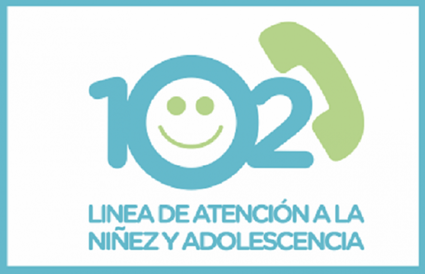
\includegraphics[width=\linewidth]{./Figuras/Ouvidorias/102-Argentina.png}}\vspace{-3pt}
  \\
  \subfloat[Vietnã\label{fig:Vietna}\vspace{-5pt}]{
\includegraphics[width=\linewidth]{./Figuras/Ouvidorias/111-Vietna.png}}\vspace{-3pt}
  \\
  \subfloat[França\label{fig:Franca}\vspace{-5pt}]{
\includegraphics[width=\linewidth]{./Figuras/Ouvidorias/119-Franca.png}}\vspace{-3pt}
  \\
  \subfloat[Aruba\label{fig:Aruba}\vspace{-5pt}]{
\includegraphics[width=\linewidth]{./Figuras/Ouvidorias/131-Aruba.png}}\vspace{-3pt}
  \\
  \subfloat[Japão\label{fig:Japao}\vspace{-5pt}]{
\includegraphics[width=\linewidth]{./Figuras/Ouvidorias/189-Japao.png}}\vspace{-3pt}
  \\
  \subfloat[Índia\label{fig:India}\vspace{-5pt}]{
\includegraphics[width=\linewidth]{./Figuras/Ouvidorias/1098-India.png}}\vspace{-3pt}
  \\
  \subfloat[Tailândia\label{fig:Tailandia}\vspace{-5pt}]{
\includegraphics[width=\linewidth]{./Figuras/Ouvidorias/1387-Thailandia.png}}
  %\begin{center}
  %  
\includegraphics[width=\linewidth]{./Figuras/Ouvidorias/100-Brasil.png}
  %\end{center}
  %\begin{center}
  %  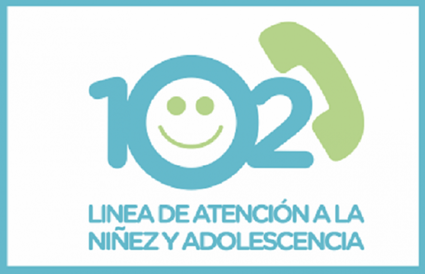
\includegraphics[width=\linewidth]{./Figuras/Ouvidorias/102-Argentina.png}
  %\end{center}
  %\begin{center}
  %  
\includegraphics[width=\linewidth]{./Figuras/Ouvidorias/131-Aruba.png}
  %\end{center}
  %\begin{center}
  %  
\includegraphics[width=\linewidth]{./Figuras/Ouvidorias/111-Vietna.png}
  %\end{center}
  %\begin{center}
  %  
\includegraphics[width=\linewidth]{./Figuras/Ouvidorias/189-Japao.png}
  %\end{center}
  %\begin{center}
  %  
\includegraphics[width=\linewidth]{./Figuras/Ouvidorias/1098-India.png}
  %\end{center}
  %\begin{center}
  %  
\includegraphics[width=\linewidth]{./Figuras/Ouvidorias/1387-Thailandia.png}
  %\end{center}
  %\begin{center}
  %  
\includegraphics[width=\linewidth]{./Figuras/Ouvidorias/119-Franca.png}
  %\end{center}
  \vspace{-8pt}
  \legend{Fonte: \citeonline{linhas2017}.}%eu paguei outros nao citados aqui, como fazer a referencia?
  %india (mas não governamental)
\end{wrapfigure}

%https://www.argentina.gob.ar/justicia/violencia-familiar-sexual [A argentina atende também por WhatsApp = Mensageiros Instantaneos (além do telefone 137 e do email vicontravio@jus.gov.ar)]

Os canais de denúncia são uma estratégia relevante no combate a violência sexual infantil. Os meios de comunicação para delação servem de alicerce para garantir os direitos legalmente estabelecidos das crianças e dos adolescentes. Entre os meios de denúncia mais amplamente presentes pelo mundo estão as linhas telefônicas. A \autoref{fig:Canais} elenca as principais ouvidorias telefônicas de alguns países.

%Canais não presenciais de atendimento (ao cidadão)

Os números telefônicos da \autoref{fig:Canais} demonstram a preocupação dos países em garantir um canal seguro de comunicação para crianças em situação de risco. A depender do país, cada canal de comunicação pode aceitar outras formas de denúncia, além da violência infantil. No caso do Brasil, o Disque 100 (Figura\autoref{fig:Brasil}), além de receber denúncias contra crianças, também recebe denúncias de outros grupos vulneráveis como idosos e deficientes. Os meios de denúncia veem no intuito de mitigar as lacunas deixadas pelas políticas públicas no que diz respeito a fiscalização.

Os canais telefônicos são instrumentos de denúncia a distância confiáveis e acessíveis \cite{linhas2017}. A penetrância dos dispositivos móveis no Brasil, torna este instrumento ainda mais poderoso no combate a violência infantil, uma vez que a quantidade de dispositivos móveis operantes no país ultrapassa a própria população brasileira. Além das denúncias por ouvidorias telefônicas, as denúncias podem ser realizadas por correio eletrônico, aplicativos e portais governamentais. As denúncias no Brasil podem ser realizadas de forma totalmente gratuita durante toda a semana 24 horas por dia (incluindo sábados, domingos e feriados).

O processo de denúncia se aplica tanto para crimes tentados quanto para crimes praticados. Deste modo, amplia-se a possibilidade de garantir a segurança e bem estar das crianças antes ou após a violência, bastando para isso, um meio de comunicação e um número telefônico. Neste sentido, cabe destacar os números de cada país são válidos apenas em caráter nacional, a linha internacional de denúncia do Brasil é: +55 (61) 3212-8400.

%Não falei do AloAloBrasil (Alo123), nem do SaferNet.


%As linhas de atendimento infantil estão no cruzamento crítico, onde crianças e jovens encontram seu caminho para a proteção e os cuidados prestados pelos sistemas de proteção infantil; eles são fontes confiáveis e acessíveis de ajuda e apoio a crianças e jovens e de encaminhamento para o sistema de proteção infantil, incluindo a aplicação da lei, se necessário\cite{linhas2017}

%https://www.unicef.org/protection/files/LEAP_report_CHI_and_UNICEF_(final).pdf \cite{linhas2017}
%https://www.police.sa.gov.au/your-safety/child-safety
%https://www.childhelplineinternational.org/child-helplines/child-helpline-network/
%\footnote{ \url{https://www.childhelplineinternational.org/child-helplines/child-helpline-network/}}


%colocar as policias antes...
\section{Propagandas}\label{sec:propagandas}

As propagandas são um mecanismo chave no combate ao abuso sexual infantil. Os meios de divulgação ajudam na dispersão do conhecimento e na conscientização da população. Os programas de conscientização da população são largamente conhecidos por auxiliarem suas respectivas lutas. %seja em capampanhas de vacinação ou em campanhas de combate a mosquitos transmissores de doenças. 
No caso do abuso sexual infantil, as propagandas auxiliam as crianças sobre seus direitos ensinando-as e encorajando-as a realizarem denúncias. Um exemplo de propaganda neste estilo é apresentado tanto na \autoref{fig:adulto} quanto na \autoref{fig:crianca}.

\begin{figure}[htb]
  %\caption{\label{fig:propagandas}Propaganda}
  \begin{center}
  \begin{minipage}[t]{0.5\textwidth}
    \caption{\label{fig:adulto}Propaganda na visão do Adulto.}
    \vspace{0.1cm}
    \centering
    \frame{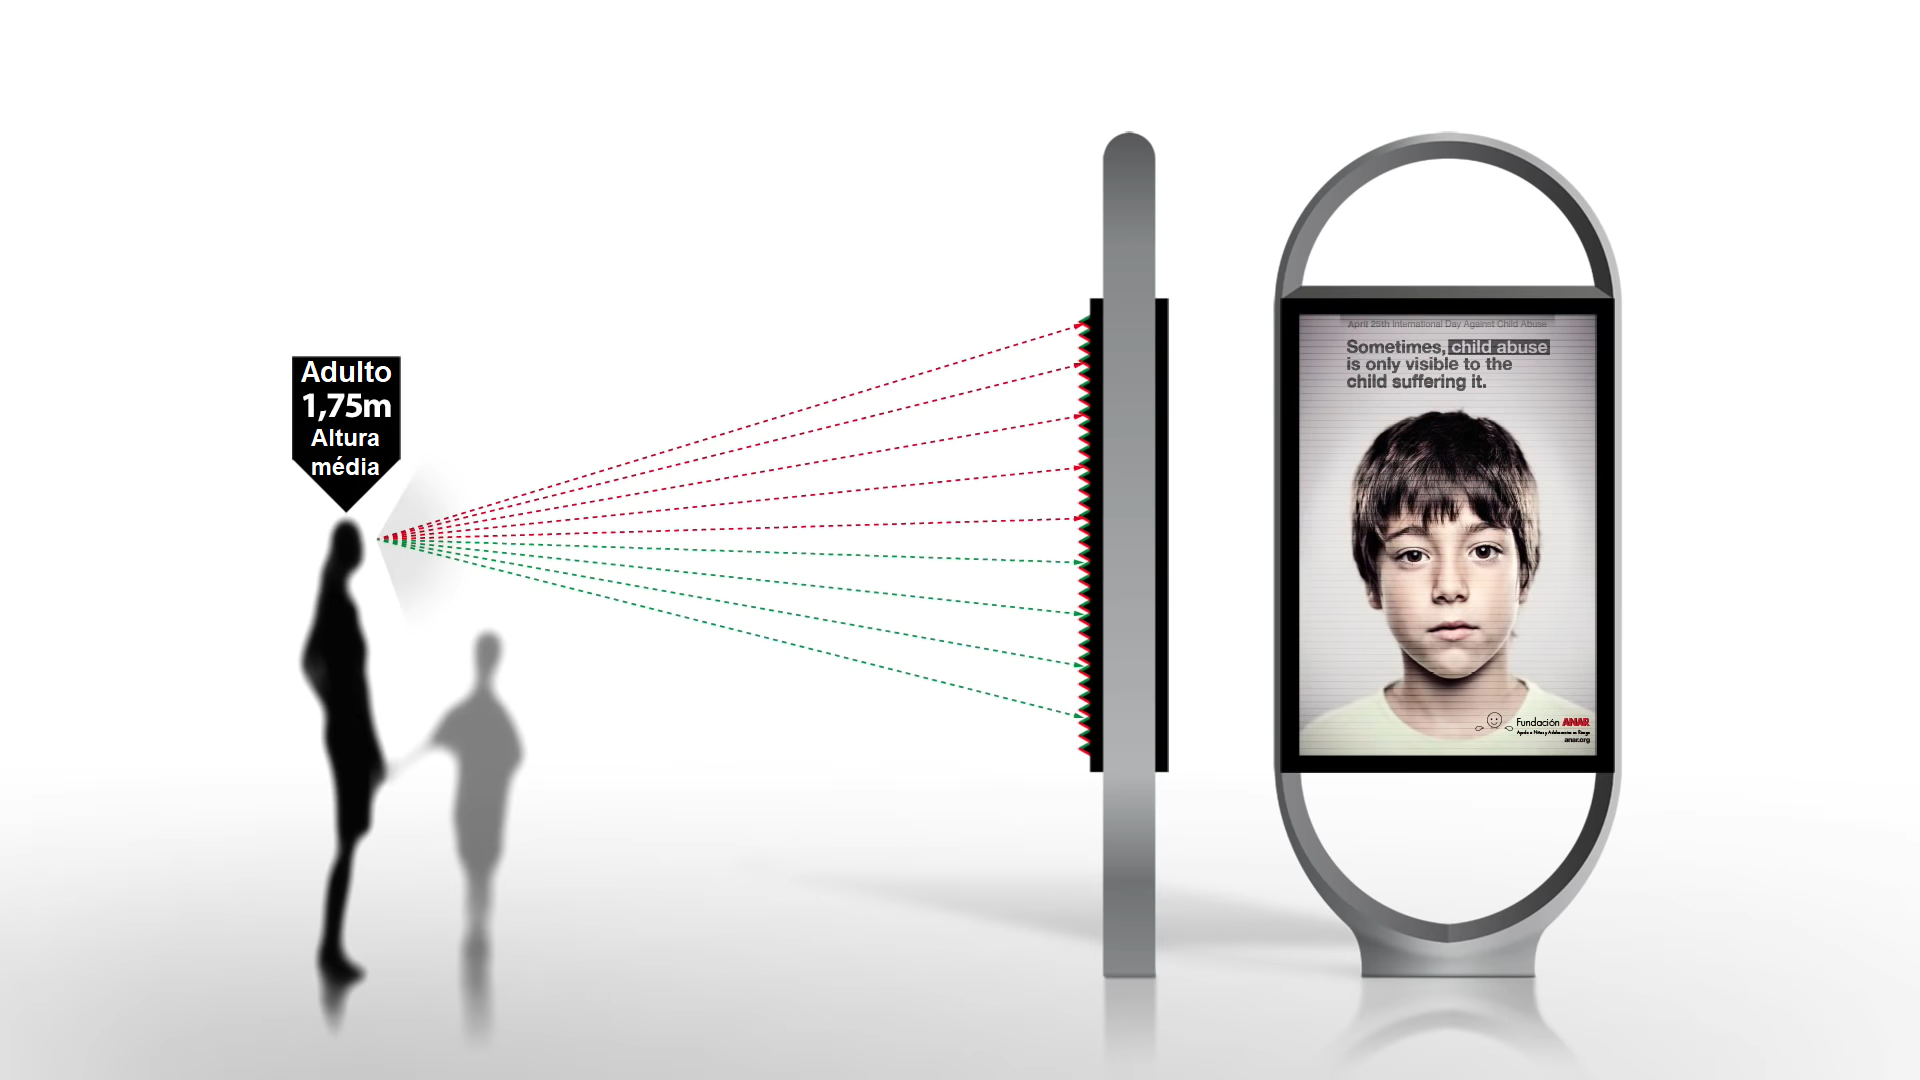
\includegraphics[width=\linewidth]{./Figuras/Propagandas/Propaganda-Adulto.png}}      
\end{minipage}%
~ 
\begin{minipage}[t]{0.5\textwidth}
    \caption{\label{fig:crianca}Propaganda na visão da Criança.}
    \vspace{0.1cm}
    \centering
    \frame{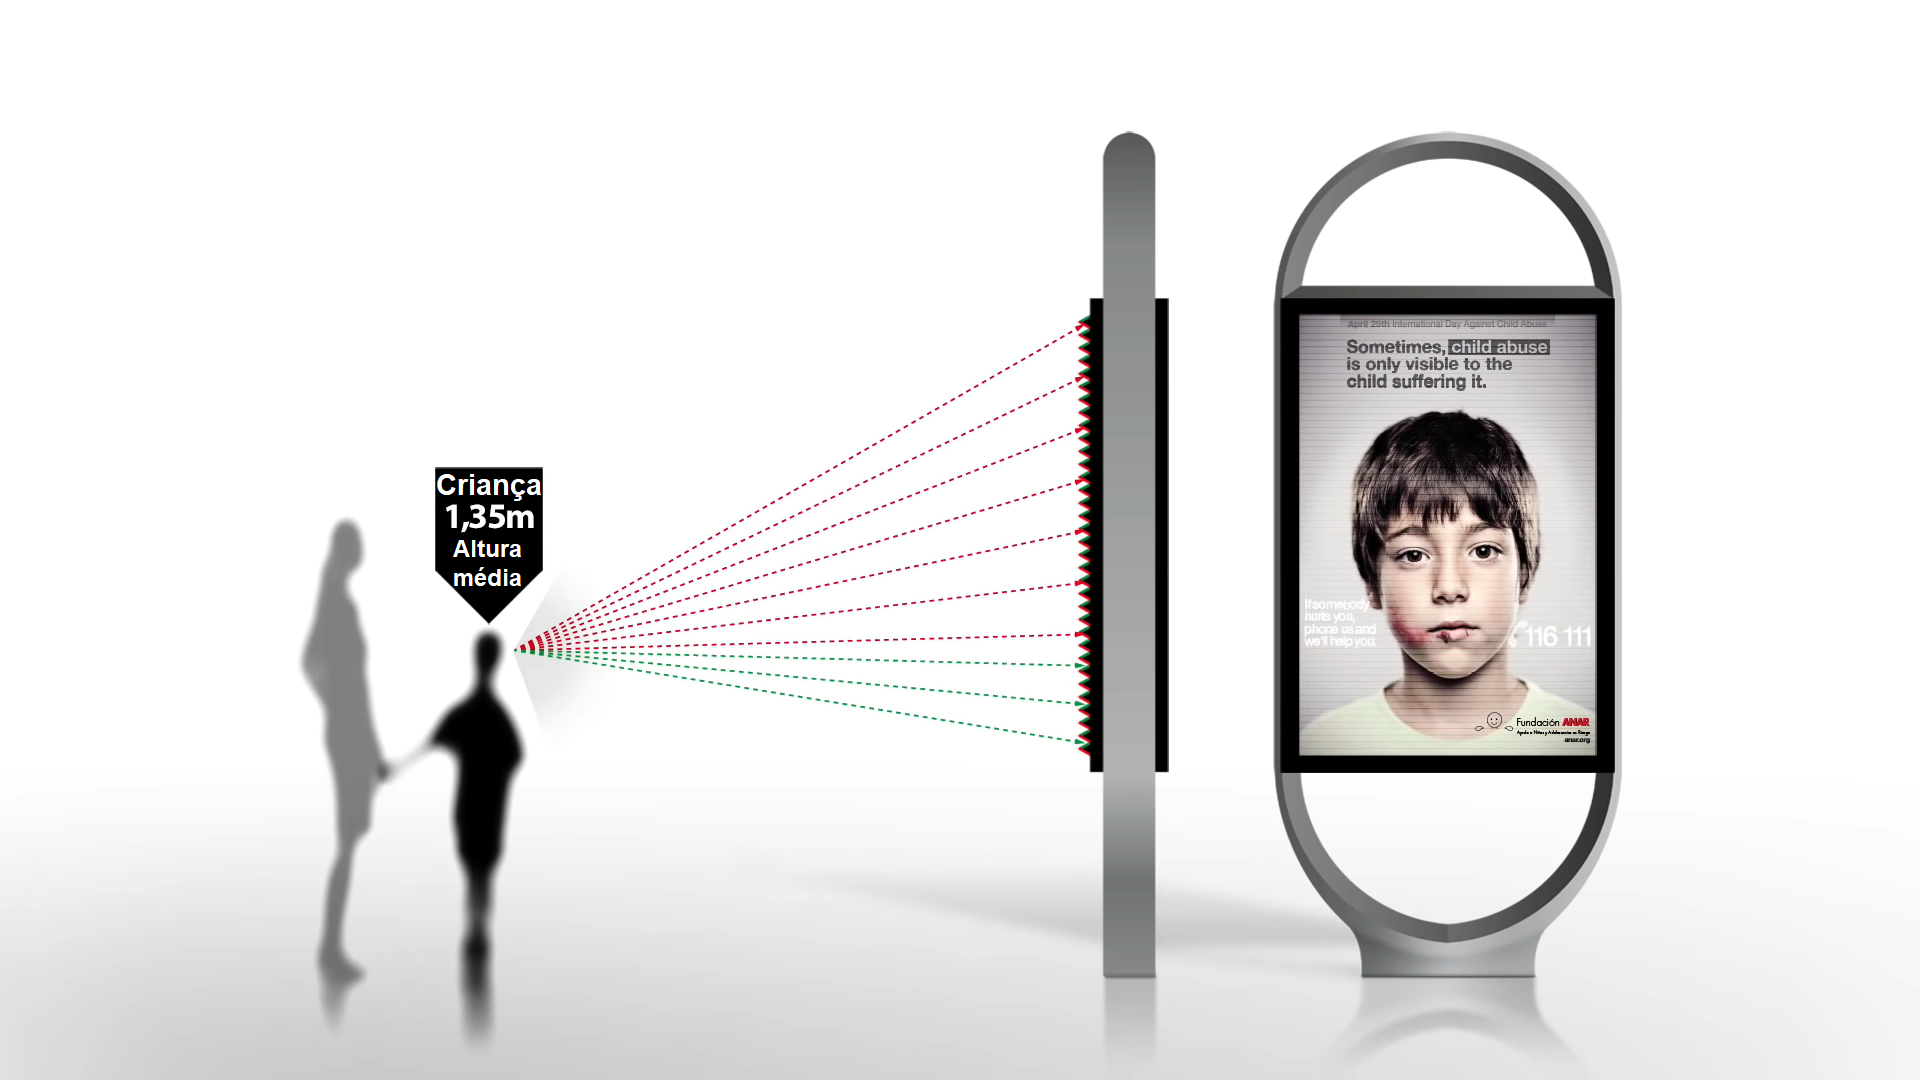
\includegraphics[width=\linewidth]{./Figuras/Propagandas/Propaganda-Crianca.png}}
\end{minipage}

	\end{center}
  \legend{Fonte: adaptado de Anar Foundation (2013)}
%https://www.youtube.com/watch?v=6zoCDyQSH0o   - Anar Foundation
%https://www.youtube.com/watch?v=N0h1mgpn95s&feature=emb_title [trocar, esse é o original]
\end{figure}
%"Si alguien te hace daño llámanos y te ayudaremos"

A \autoref{fig:adulto} e a \autoref{fig:crianca} apresentam a mesma propaganda, porém vista de ângulos diferentes. A propaganda parte da concepção de que muitas crianças violentadas transitam pelas ruas com seus próprios agressores. Agressores estes, que para não serem encarcerados garantem o desconhecimento da criança sobre os meios de denúncia relativos ao crime cometido. A propaganda então, baseada sob estes princípios, apresenta uma mensagem visível apenas a partir do ângulo de visão da altura média de uma criança (1,35 metros). A mensagem, dentre outras informações, apresenta aos menores um número telefónico, o qual permite um canal de ajuda e socorro as crianças vítimas de violência. 

As propagandas auxiliam na divulgação de informações, as quais capacitam as pessoas a reconhecerem o problema e a reagirem adequadamente ao problema. Os meios de comunicação são os mais variados, podendo ir desde comerciais no rádio, na televisão ou na internet \cite{martinez2011prevencion}. Além disso, excelentes meios de divulgação são cartazes, panfletos, cartilhas e campanhas governamentais \cite{mendelson2015parent}.


%``Existe una gran variedad de opciones metodologicas al alcance de los usuarios. Dentre de estas, las mas utilizadas han sido los \textbf{materiales impresos, los videos o materiales audiovisuales, las charlas, las representaciones teatrales y el role playing}'' (corrigir erros do espanhol) [Esse artigo é bom, pois fala dos toque bons, toque ruins, partes íntimas, etc] ... ``el abusador impone a el nino ley de silencio (segredo)'' ... ``los programas deberian poner el acento en transmitir a los ninos la importancia de divulgar el abuso y no en pedirles que se nieguen y sean capaces de deternerlo'' [LEMBRA DO JOGO TRIALHA DA PROTEÇÃO, ao completar a criança recebe o título de 'PROTEGIDO'] \cite{martinez2011prevencion} 


\section{Atendimento Hospitalar}\label{sec:hospital}

Os atendimentos hospitalares são procedimentos poderosos no combate aos maus tratos contra as crianças. O profissional de saúde surge como um sujeito ativo, no sentido de identificar abusos e denunciá-los, conforme ordena a legislação brasileira \cite{costa2019maus}. Inúmeros jornais e portais de notícias já relataram inclusive o diagnóstico de violência sexual infantil em laudos médicos\footnote{Redação de Notícias Catve.com (28/12/2018): \url{https://catve.com/noticia/9/238135/menina-de-11-anos-e-internada-com-dores-abdominais-e-medico-descobre-gravidez}.}\footnote{Portal de Notícias G1 (08/08/2018): \url{https://g1.globo.com/ro/ji-parana-regiao-central/noticia/2018/08/08/mae-leva-filha-de-5-anos-ao-pediatra-e-descobre-que-menina-foi-estuprada-em-ro.ghtml}.}\footnote{Jornal Metropóles (07/06/2016): \url{https://www.metropoles.com/distrito-federal/seguranca-df/medico-denuncia-estupro-de-menina-de-11-anos-em-festa-de-escola-no-df}.}\footnote{Rede Jornalística A Gazeta (03/11/2017): \url{https://www.gazetaonline.com.br/noticias/policia/2017/11/menino-contrai-sifilis-e-familia-descobre-abuso-sexual-1014106068.html}.}\footnote{Portal de Notícias G1 (26/08/2015): \url{http://g1.globo.com/sao-paulo/itapetininga-regiao/noticia/2015/08/mae-descobre-que-filho-foi-estuprado-apos-dentista-achar-doenca-na-boca.html}.}\footnote{Portal de Notícias G1 (23/04/2013): \url{http://g1.globo.com/sp/bauru-marilia/noticia/2013/04/exame-aponta-que-menina-de-3-anos-sofreu-abuso-sexual-em-bauru-sp.html}.}.%\footnote{Correrio do Estado (31/07/2019): \url{https://www.correiodoestado.com.br/cidades/exame-aponta-doenca-e-tia-descobre-estupro-de-criancas/357839/}}\footnote{Portal G1 (08/08/2019): \url{https://g1.globo.com/sp/sao-jose-do-rio-preto-aracatuba/noticia/2019/08/08/pais-tiram-crianca-de-hospital-antes-de-alta-apos-medico-suspeitar-de-sinais-de-abuso-sexual.ghtml}}.

%https://g1.globo.com/bahia/noticia/crianca-de-oito-anos-morre-por-insuficiencia-respiratoria-apos-estupro.ghtml [mórbido demais para citar, eu acho]

%https://www.google.com/url?sa=t&rct=j&q=&esrc=s&source=web&cd=8&cad=rja&uact=8&ved=2ahUKEwia2sGezbHpAhUND7kGHcVjDx4QFjAHegQICBAB&url=https%3A%2F%2Fwww.radiocacula.com.br%2Fnoticias%2Fcidades%2Fmenina-de-4-anos-morre-medico-descobre-estupro-e-pai-e-o-suspeito&usg=AOvVaw0k64eNQ83eicbnl4eJGl55 [mórbido demais para citar, eu acho]

A literatura médica comenta sobre a dificuldade em constatar sinais de violência infantil em alguns casos. Em certas circunstâncias se exige do médico muito mais perspicácia e experiência profissional \cite{de2012violencia}. Devido a complexidade no diagnóstico de alguns episódios de abuso, guias clínicos foram desenvolvidos como o Guia Clínico da Organização Mundial da Saúde \cite{world2017responding}. Os relatórios e guias médicos são capazes de ajudar os profissionais de saúde a identificar mais facilmente sinais de abuso acometidos contra a criança e contra o adolescente \cite{Christian1}.

%``This guideline aims to provide evidence-based recommendations for quality clinical care for children and adolescents who have, or may have, been subjected to sexual abuse, in order to mitigate the negative health consequences and improve their well-being. The objectives are to support health-care providers to provide quality, immediate and long-term clinical care and to apply ethical, human-rights-based and trauma-informed good practices in the provision of such care. Where relevant for provision of clinical care and where there is supporting evidence, sex-based differences and gender-based inequalities are flagged.''\cite{world2017responding}

%``the report can help primary care pediatricians learn clinical clues to the diagosis of abuse and undertand specific injuries of concern, appropriate diagnostic testes and considerations, and legal requirements related to mandated reporting of suspected abuse'' \cite{Christian1}

Os guias e relatórios médicos ajudam tanto no diagnóstico, quanto na procedência dos tramites legais. Nos casos agudos de violência sexual, com menos de 72h do ocorrido, as medidas legais já devem acompanhar toda a assistência inicial de diagnóstico e tratamento. Nos casos crônicos e repetitivos, sem grandes lesões visíveis, será fundamental o registro de anamnese, histórico familiar e dados de exame físico. Para fins de processo judicial e a necessária comprovação da agressão, bem como para confecção de exames que levem à identificação do agressor, é preciso que os responsáveis façam um boletim de ocorrência em delegacia de polícia, que requisitará o laudo pericial do Instituto Médico Legal \cite{de2012violencia}. 

O atendimento hospitalar adiciona mais uma camada de defesa no enfretamento a violência sexual infantil. Embora os abusos só possam ser diagnosticados após sua ocorrência, a defesa médica ainda se faz válida para diminuir a reincidência dos eventos abusivos, seja em um exame de rotina ou qualquer outra forma de atendimento \cite{costa2019maus}.

%``No atendimento do consultório odontológico o cirurgião-dentista pode encontrar crianças com lesões características de violência física, seja em um exame de rotina ou qualquer outra forma de atendimento''\cite{costa2019maus}

%\cite{christian2015evaluation}

%O método clínico, composto pela anamnese e o exame físico e auxiliado por exames complementares, é o maior arsenal que o médico dispõe para o diagnóstico de maus tratos ou violência infantil \cite{de2012violencia}.

%http://www2.fm.usp.br/gdc/docs/iof_152_5-violencia.pdf [LER]
%https://repositorio.unb.br/bitstream/10482/2302/1/Sonia%20Fortes%20do%20Prado.pdf



\section{Centros de Tratamento às Vítimas}\label{sec:centros}

%Resultados da pesquisa Trecho da Web em destaque O Centro de Referência às Vítimas de Violência (CRVV) é um serviço do Município, em parceria com o Governo Federal, criado para prestar informações e orientações às vítimas de violações de direitos, abuso de autoridade, exploração sexual e qualquer tipo de discriminação.

Os centros de tratamento estabelecem uma poderosa estratégia de enfretamento ao maltrato infantil. No Brasil, o tratamento e recuperação da criança vítima de violência pode ser executado pelo Conselho Tutelar. Os Conselhos Tutelares estão para a violência sexual infantil e adolescente, como as equipes de resgate estão para os primeiros socorros \cite{caccia2014conselheiros}.

%Art. 131. O Conselho Tutelar é órgão permanente e autônomo, não jurisdicional, encarregado pela sociedade de zelar pelo cumprimento dos direitos da criança e do adolescente, definidos nesta Lei (ECA). 

O Conselho Tutelar é um órgão permanente e autônomo, não jurisdicional, encarregado de zelar pelo cumprimento dos direitos da criança e do adolescente \cite{saude2002notificacao}. Além do Conselho Tutelar, a nível nacional ainda é possível citar o Centro de Referência Especializado de Assistência Social (Creas), responsável pelo acolhimento e pelo atendimento a famílias e indivíduos em situação de risco pessoal e social, por violência, abuso e exploração sexual, ocorrência de abandono, maus-tratos físicos e/ou psíquicos, cumprimento de medidas socioeducativas, situação de rua e de trabalho infantil, entre outras situações de violação dos direitos.

Os centros de tratamento não são uma exclusividade apenas do Brasil. Estratégias do gênero podem ser encontradas em várias países pelo globo, como: Madri\footnote{ Centro especializado de Intervención en abuso sexual infantil (CIASI): \url{http://edicion.comunidad.madrid/servicios/asuntos-sociales/intervencion-abuso-sexual-infantil}.}, Equador\footnote{Centro Integral de la Niñez y Adolescencia (CENIT): \url{http://cenitecuador.org/}.} %que é uma organização sem fins lucrativos
e Argentina\footnote{Centro Integral Especializado en Niñez y Adolescencia (CIENA): \url{https://www.buenosaires.gob.ar/desarrollohumanoyhabitat/mujer/hogares-y-centros-integrales-de-la-mujer/asistencia-al-maltrato-infantil}.}. Embora os objetivos dos centros sejam similares, a estrutura organizacional e operacional pode variar bastante de centro para centro. No caso do Brasil, a lei obriga que exista pelo menos um Conselho Tutelar por município composto de pelo menos cinco membros com idoneidade moral escolhidos pela comunidade local. %https://www.mpdft.mp.br/portal/pdf/unidades/promotorias/pdij/Conselhos/guia_conselheirotutelar11.pdf

O Conselho Tutelar e demais centros de tratamento veem na perspectiva de atuar diante dos maus-tratos sem se limitar ao tratamento médico dos traumas e lesões resultantes desses problemas \cite{brasil2002notificaccao}. A implementação de centros do gênero estabelece um grande aliado na proteção dos direitos da infância e da juventude e a sua implementação no país é de extrema importância para o enfrentamento à violência contra crianças e adolescentes. %https://www.childhood.org.br/conquistas-do-eca-criacao-do-conselho-tutelar
O Conselho Tutelar não presta o atendimento direto, mas atua de forma que ele se viabilize em casos concretos de ameaça ou violação de direitos. O ECA prevê que os casos de suspeita ou confirmação de maus-tratos contra criança ou adolescente serão obrigatoriamente comunicados ao Conselho Tutelar da respectiva localidade, sem prejuízo de outras providências legais.

%Centros de Referências em Assistência Social – CREAS e Centros de Atendimento Psicossocial – CAPS, esses centros são acionados para atendimento psicossocial e de assistência social e também para encaminhamentos de casos de drogadição.


%``Abuso sexual: consiste em todo ato ou jogo sexual, relação heterossexual ou homossexual cujo agressor está em estágio de desenvolvimento psicossexual mais adiantado que a criança ou o adolescente. Tem por intenção estimulá-la sexualmente ou utilizá-la para obter satisfação sexual. Apresenta-se sobre a forma de práticas eróticas e sexuais impostas à criança ou ao adolescente pela violência física, ameaças ou indução de sua vontade. Esse fenômeno violento pode variar desde atos em que não se produz o contato sexual (voyerismo, exibicionismo, produção de fotos), até diferentes tipos de ações que incluem contato sexual sem ou com penetração. Engloba ainda a situação de exploração sexual visando lucros como é o caso da prostituição e da pornografia.'' \cite{saude2002notificacao} [Essa referencia também explica um pouco sobre o conselho Tutelar]


\section{Departamentos Policiais}\label{sec:dp}%ARRUMAR - CADA ESTADO É UMA DELEGACIA

%Cada estado parece ter a sua, ver a lei que define isso, definir de qual estado é a DPCA, aqui em santa catarina parece que temos a DPCAMI


As delegacias especializadas são um bom artifício de confronto a violência sexual infantil. A Delegacia de Proteção à Criança e Adolescente (DPCA) é competente para fiscalizar, investigar e instaurar inquérito e procedimentos policiais nos casos de infração penal praticada contra crianças e adolescentes. Isso significa que a DPCA é responsável por crimes em que as crianças e adolescentes são as vítimas e não autores do delito. Além desta função, a DPCA também desenvolve estratégias de repressão continuadas em qualquer local, público ou privado, como forma de interromper o ciclo de impunidade dos agressores \cite{rodrigues2014}. %Toda prática de violência contra criança ou adolescente deve ser denunciada nesta delegacia especializada. Não é necessário se identificar para comunicar algum crime 

As delegacias especializadas são consideradas determinantes no processo de visibilidade da violência sexual contra crianças e adolescentes \cite{plano2013}. Não à toa, sua presença se alastra por outros países ao redor do mundo, como por exemplo: Colombia\footnote{Delegacia da Infância e Adolescência (Policía de Protección a la Infancia y Adolescencia).}, Índia\footnote{Special Juvenile Police Units (SJPU).} e França\footnote{Brigade de protection des mineurs.}.
%BRASIL: Delegacia de Proteção à Infância e Adolescência
%Colombia: 
%India? : Special Juvenile Police Units(SJPU) %http://www.wcddel.in/Guidelines[1].pdf
%França: Brigade de protection des mineurs: %https://www.prefecturedepolice.interieur.gouv.fr/Nous-connaitre/Services-et-missions/Missions-de-police/La-direction-regionale-de-la-police-judiciaire/La-brigade-de-protection-des-mineurs
Não há uma diretriz operacional única entre as delegacias especializadas, nem mesmo a nível nacional. No Brasil, algumas delegacias ficam abertas 24 horas por dia todos os dias da semana, enquanto outras operam apenas nos dias úteis e em horário comercial. E mesmo as abertas 24 horas não possuem uma equipe multidisciplinar de plantão, contando com apenas os funcionários essenciais para o registro da ocorrência como agentes, escrivães e delegado \cite{novo2016}. 

Boa parte das iniciativas de criação de DPCAs ainda são muito recentes, ressaltando-se a carência tanto de legislação específica quanto de pesquisas e material especializado publicados sobre elas \cite{novo2016}. Isso ajuda a explicar melhor as divergências encontradas entre as delegacias no que diz respeito a presença ou não de carceragem, brinquedoteca e salas de atendimento psicológico. 
%meio que todas tem briquedoteca, mas é tipo um chuncho
Em adendo, algumas Delegacias relataram convênios com hospitais, universidades e Organizações Não Governamentais.

As delegacias especializadas integram o Sistema de Garantias dos Direitos da Criança e do Adolescente. Essas delegacias ainda podem se dividir entre as voltadas para o atendimento às vítimas ou voltadas para a lidar com os infratores, havendo ainda aquelas que conjugam as duas funções em um mesmo órgão. A efetividade dos mecanismos de denúncia e notificação garante a possibilidade não apenas de atendimento às vítimas, mas também de responsabilização e tratamento dos agressores, evitando a impunidade e o ciclo repetitivo da violência \cite{novo2016}.

%DPCA – DELEGACIA DE PROTEÇÃO À CRIANÇA E AO ADOLESCENTE
%DPAI - Delegacia de Polícia do Adolescente e outras

%https://www.camara.leg.br/noticias/604913-comissao-aprova-notificacao-obrigatoria-de-maus-tratos-e-automutilacao-de-criancas/ [NOTIFICACAO OBRIGATORIA]

%O Sistema de Garantia dos Direitos da Criança e do Adolescente compreende oscentros de defesas, as delegacias especializadas, a vara da infância e juventude, aspromotorias da infância e juventude, conselho tutelar, conselho de direitos, dentre outros. Ésalutar apresentar informações alusivas a estas instituições, já que podem ser acionadasquando da denúncia de abuso sexual \cite{rodrigues2014}.


\section{Operações Policiais}\label{sec:op}

As operações policiais são excelentes alternativas na luta contra o abuso e a exploração sexual infantil. No Brasil e no mundo as operações são responsáveis pela busca e apreensão de inúmeros criminosos sexuais, o que acaba por mitigar a reincidência do crime por parte destes agressores. 

A literatura relata a Operação Carrossel (2007) como o primeiro esforço policial internacional a combater a pornografia infantil na internet \cite{lowenkron2014all}. Todavia, há registros anteriores que relatam a mesma abrangência policial internacional, como a Operação Catedral (1998) objetivada também no combate a pornografia infantil na internet \cite{Barrot2008, jesus2006anti}. É importante destacar que isto não se trata necessariamente de uma contradição literária, a Operação Darknet (2014) também é descrita como pioneira no combate a distribuição de material pornográfico infanto-juvenil na internet, contudo o pioneirismo desta, configura-se pela metodologia de investigação e pelas ferramentas para identificar usuários criminosos na DeepWeb \cite{tonello2018pedofilia}. Ou seja, cada operação pode ser classificada como pioneira com base em seus contextos específicos. 

%A Agência de Notícias da Polícia Federal apresenta dados sobre a operação Darknet, investigação pioneira, que objetivou combater uma rede de distribuição de pornografia infanto-juvenil na Darkweb, foi deflagrada pela polícia Federal em 2014 e 2016. Na primeira fase foram cumpridos 93 mandados de busca e na segunda fase 70. A Polícia Federal antecipou o cumprimento de 7 ordens judiciais para evitar o possível abuso sexual de crianças. Desde a primeira fase da Operação Darknet (2014), a Polícia Federal desenvolve metodologia de investigação e ferramentas para identificar usuários da DarkWeb, considerado um meio seguro de divulgação de conteúdos variados de forma anônima. A arquitetura desse ambiente impossibilita a identificação do ponto de acesso (IP), ocultando o real usuário que acessa a rede. Poucas polícias no mundo obtiveram êxito em investigações na Darkweb, como o FBI, a Scotland Yard e a Polícia Federal Australiana \cite{tonello2018pedofilia}.

%depois de seis meses de uma ação integrada em prol do combate a crimes de exploração sexual contra crianças, chamada de Operação Luz na Infância 2, foram presas, em maio de 2018, 21 pessoas, incluindo uma criança, na posse de material com conteúdo de exploração sexual infanto-juvenil. Em Porto Alegre, foram oito prisões, duas em Santa Maria, duas em Cachoeirinha e duas em Novo Hamburgo, além de prisões efetuadas em Alvorada, Pelotas, Panambi, Taquara, Canoas, Sapucaia, São Leopoldo e Viamão. Também foram apreendidos diversos computadores, notebooks, HDs externos, pendrives e outros dispositivos de armazenamento que continham material referente a crimes de abuso e exploração sexual infanto-juveni \cite{tonello2018pedofilia}.

No Brasil, o Ministério da Justiça considera a Operação Luz na Infância (2017) como a maior operação do gênero no Brasil e na América Latina. Isto, pois a operação é um conglomerado de vários países e instituições \cite{souza2018sabemos}. Entre os países estão: Brasil, Chile, El Salvador, Equador, Estados Unidos, Panamá e Paraguai. A Operação já teve mais de cinco fases apreendendo um volume total de dados que ultrapassa os três terabytes, além da prisão de mais de 500 indivíduos. 

%A Polícia Federal já deflagrou algumas operações que tinham como objetivo combater a pedofilia na internet. As primeiras foram as intituladas como Carrossel I (2007) e Carrossel II (2008). E em outubro de 2017, a Operação Luz na Infância, que foi considerada pelo Ministério da Justiça, a maior operação que houve no Brasil e na América Latina, de acordo com a matéria do jornal a Folha (2017). \cite{souza2018sabemos}

As operações policiais são políticas públicas de segurança que estão fundamentadas e baseadas nos limites da legislação e da jurisdição de suas nações, resguardados os acordos internacionais. Dito isso, é notória a dependência que as operações policiais possuem com o âmbito jurídico. Se não há tipificação legal do crime, então não a crime a ser reprimido. Por tal razão que a sansão de decretos e a criação de leis neste contexto se fazem fundamentais para o fortalecimento das operações policiais. 

%Em 8 de maio de 2017, foi sancionada a Lei de Nº 13.441 que altera a lei do ECA e prevê a infiltração de agentes de polícia na internet com o fim de investigar crimes contra a dignidade sexual de crianças e adolescentes (BRASIL, 2017). \cite{souza2018sabemos}

%Operação Luz na Infância (2018) (7 países) \cite{souza2018sabemos}
%Operação Tapete Persa (2010) \cite{da2012bibliotecas} \cite{barros2014pedofilia}
%Operação Darknet (2014) %http://www.mpf.mp.br/rs/sala-de-imprensa/docs/outros-documentos/operacao-darknet
%Operação Carrossel (2007) \cite{souza2018sabemos}
%Operação Alanis (2016)

%Operation Netsafe (2017) Reino Unido (wales) %https://www.gwent.police.uk/en/newsroom/operations-campaigns/operation-netsafe/ %https://www.south-wales.police.uk/en/advice/child-sexual-exploitation-cse/operation-net-safe-tackling-online-child-sexual-abuse-and-exploitation/

%Operação Atelier (2014) EUROPOL %https://www.europol.europa.eu/activities-services/europol-in-action/operations/operation-atelier

%OPERATION RESCUE (2011) EUROPOL %https://www.europol.europa.eu/activities-services/europol-in-action/operations/operation-rescue

%OPERATION ATLANTIC (2010) EUROPOL %https://www.europol.europa.eu/activities-services/europol-in-action/operations/operation-atlantic

%OPERATION ICARUS (2011) EUROPOL %https://www.europol.europa.eu/activities-services/europol-in-action/operations/operation-icarus

%OPERATION ARCHIMEDES = EUROPOL + INTERPOL

%Operação Catedral (1998) (12 países) \cite{jesus2006anti} [aqui fala da operação e como legislar sobre um site que opera em um país mas está hospedado em outro]


%http://www.pf.gov.br/agencia/noticias/2014/10/pf-combate-a-disseminacao-de-pornografia-infantil-pela-deep-web-no-rs

A dependência jurídica das operações policiais pode ser uma barreira a ser enfrentada no combate a violência sexual infantil. De nada adianta uma operação contra o abuso de crianças em um país que permite legalmente o casamento infantil. Além da barreira jurídica, as estratégias policiais sofrem do mesmo mal dos atendimentos hospitalares, uma vez que a apreensão do criminoso só pode ocorrer após a ocorrência do crime ou a tentativa dê, todavia a defesa policial ainda se faz válida para diminuir a reincidência dos eventos abusivos uma vez que os criminosos tenham sido encarcerados ou levados a tratamento. 

%apenas para deixar claro, eu acho que a legislação é necessária, eu apenas gostaria que ela fosse mais baseada na ciência do que em achismos ou costume culturais. 

%Aqui abaixo vemos a \textbf{estratégia da Alemanha} em produzir pornografia infantil %falsa:
%\begin{itemize}
%  \item https://www.zdf.de/nachrichten/heute/%lambrecht-will-ermittlern-herstellung-gefakter-kinderpornografie-erlauben-100.html
%
%  \item https://www.dw.com/en/germany-plans-to-use-fake-child-porn-to-snare-pedophiles/%a-51361810
%
%  \item https://www.terra.com.br/noticias/%alemanha-planeja-usar-pornografia-infantil-falsa-para-capturar-pedofilos,%869a166ee7af97bb44f30200b7f93597y5krakph.html
%\end{itemize}

%A alemanha quer produzir pornografia infantil para capturar pedófilos (isca)

\section{Gestão de Infratores}\label{sec:infratores}

%O tratamento pode ser orientado para a componente comportamental, cognitivo-comportamental, psicossocial, medicação anti androgénica ou castração.

A gestão de agressores sexuais é um bom meio de combate aos maus tratos infantis. Os programas de tratamento apresentam uma taxa de sucesso alta, implicando assim em uma baixa reincidência dos crimes sexuais \cite{ribeiro2018programas}. Meta-análises apoiam inclusive os efeitos significativos de tratamentos baseados em princípios cognitivo-comportamentais \cite{mendelson2015parent}.

%embora alguns estudos concluíram que as evidências não são suficientes para apoiar a eficácia dos tratamentos\cite{mendelson2015parent}

Os agressores sexuais apresentam taxas de reincidência elevadas pois durante o cumprimento da pena de prisão, nem sempre existe uma intervenção dirigida para esta problemática \cite{ribeiro2018programas, finkelhor2009prevention, maia2014castraccao}. A atitude unicamente punitiva de sistemas jurídicos, acaba por não tratar devidamente o problema do abuso sexual \cite{Camila2019}. Embora a atração sexual por crianças e adolescente seja considerada uma patologia, o agressor sexual não é considerado inimputável perante a justiça, caso o delito tipificado em lei seja cometido \cite{ribeiro2018programas}. Contudo, um tratamento adequado ao agressor se faz necessário para diminuir a probabilidade da reincidência do crime. 

As terapias e os tratamentos aos agressores sexuais precisam ser realizados com muita cautela. Por mais que os delitos cometidos pelos agressores sexuais sejam desumanos e atentem contra o livre direito de suas vítimas; por questões éticas ainda se faz necessário garantir que os tratamentos e que as terapias não violem os direitos dos agressores sexuais \cite{finkelhor2009prevention}. Por tal razão terapias de aversão ou tratamentos de castração química não são recomendadas por algumas instituições de saúde \cite{maia2014castraccao}.
%Some observers, though, argue that registration, like a lot of offender management practices, makes it harder for offenders to reintegrate into society and violates the rights of those who have already paid their debt to society

%"redirecionamento masturbatório"???

%Expressar empatia e compreensão com as pessoas que cometeram violência sexual frequentemente é visto como se estivéssemos defendendo o abusador e não a criança, contudo especialistas defendem a humanização do agressor para um tratamento adequado.

%[CASTRACAO QUIMICA] https://servicos.unitoledo.br/repositorio/handle/7574/900

Existem inúmeros métodos de tratamento e gestão de agressores sexuais, dentre eles citam-se os Círculos de Suporte e Responsabilização (CoSA – Circles of Support and Accountability), que nada mais são do que grupos de voluntários com supervisão profissional para apoiar criminosos sexuais na reintegração à sociedade após a sua soltura. Os Círculos de Suporte e Responsabilização são considerados um caso de sucesso, revelando uma taxa 70\% menor de re-ofensas para os agressores sexuais \cite{finkelhor2009prevention}. No outro sentido, existem tratamentos de apoio a indivíduos não incidentes que são sexualmente atraídos por crianças, como o projeto: Prevention Project Dunkelfeld. Esforços deste gênero produziram efeitos promissores relatados por estudos na área \cite{mendelson2015parent}.

%David Finkelhor, defende duas estratégias: \textbf{[offender management and school-based educational programs}] ``All states now have electronic sex offender registries. One goal of these registries is to allow more rapid apprehension of re-offenders; another is to prevent crime by deterring existing and future offenders. Some observers, though, argue that registration, like a lot of offender management practices, makes it harder for offenders to reintegrate into society and violates the rights of those who have already paid their debt to society, particularly those forced to register retroactively'' ... ``But though the study linked registration with reduced offending among first-time offenders, it found increased offending among those who were already registered, suggesting a possible boomerang effect from the stigma (increased difficulty finding jobs and housing, for example)'' \cite{finkelhor2009prevention}

%
%\begin{enumerate}
%  \item \cite{finkelhor2009prevention}
%
%\item .[Offender Registration] = Dados de criminosos já soltos guardando seus %registros (mais fácil de fazer a busca em caso e reincidência)
%
%\item .[Community Notification] = Lei de Megan (informar os vizinhos)
%
%\item .[Mandatory Background Checks] = Entrevistas de trabalho notificadas %(impossibilitanto o trabalho com crianças para abusadores)
%
%\item .[Residency Restrictions] = lei de Jessica (proibe os criminosos de acessarem %determinados locais, etc)
%
%\item .[Sentence Lengthening and Civil Commitment] = Alongamento de sentenças...
%
%\item .[Enhanced Detection and Arrest] = aumento dos esforços policiais para divulgar, %investigar e prender criminosos
%
%\item .[Mental Health Treatment] = terapias e tratamentos para criminosos
%
%\item .[Community Reintegration and Supervision] = Circles of Accountability and %Support (CoSA) grupos de voluntários com supervisão profissional para apoiar os %agressores sexuais à medida que se reintegram à sociedade após serem libertados do %encarceramento.
%\end{enumerate}

%[lei nao aprovada] = atualiza o Estatuto da Criança e do Adolescente (ECA — Lei 8.069, de 1990) para determinar que o juiz, ao verificar a hipótese de maus-tratos, opressão ou abuso sexual cometidos pelos pais ou responsáveis, poderá determinar como medida cautelar, além do afastamento do agressor da residência, também o seu ingresso em programas de recuperação, reeducação e prevenção de violência contra crianças ou adolescentes.

O tratamento pode ajudar que não haja novas vítimas e para que aqueles que já cometeram algum crime não voltem a fazê-lo. Demonstram-se como um excelente meio de resolução do problema, pois o problema não é resolvido simplesmente com a punição do agressor, mais sim, com o seu tratamento. 



\section{Programas de Capacitação}\label{sec:programas}



%Os programas de capacitação sao otimos nesse negocio. Podem ser citados programas de capacitam de médicos, funcionarios públicos, agentes policiais, etc etc... Porém, estes programas atuam mais na prevenção secundária ou terciairia a depender. Os programas da presente seção são focas na prevenção primaria. 

Os programas de capacitação demonstram-se como uma excelente alternativa para o enfrentamento aos maus tratos contra os menores. O processo de capacitação busca instruir determinados indivíduos sobre um certo âmbito. No caso da violência infantil, de modo geral os programas buscam ensinar um conjunto de indivíduos a identificar e reagir adequadamente ao problema. 

Os processos de capacitação podem envolver desde uma grande comunidade até grupos específicos de indivíduos. Neste sentido, a atual seção apresenta os três grupos mais corriqueiramente relatados pela literatura na área: os pais das crianças (\autoref{ssec:pais}), os profissionais que trabalham com crianças (\autoref{ssec:professores}) e as próprias crianças (\autoref{ssec:alunos}).

%https://www.gov.br/mdh/pt-br/assuntos/noticias/2020-2/junho/balanco-anual-disque-100-atendeu-2-7-milhoes-de-ligacoes-em-2019/copy_of_Relatorio_Disque_100_final.pdf



\subsection{Pais}\label{ssec:pais}



%O \underline{cuidado }p\underline{arental} é um mecanismo presente em algumas espécies que, no geral, rege a afeição existente entre a proble e seus genitores \cite{manfroi2011comportamento}. Na caso da espécie humana(taxonomicamente \textit{Homo sapiens}) o mecanismo de cuidado parental tornou-se fundamental ao longo da história evolutiva, uma vez que recém-nascidos nascem bastante imaturos e totalmente dependentes de terceiros para a sua sobrevivência. Logo, para que o ciclo evolutivo continue, é dever dos pais dar cuidado e proteção a seus filhos até alcançarem a fase adulta. Contudo, infelizmente estudos revelam duas lacunas principais que acabam por dificultar os cuidados infantis.

%Pesquisa na área de violência infantil demonstram que mais de 20\% dos pais ou padatros são os responsáveis pela violência sexual de seus próprios filhos. Já, entre os pais não agressores, pesquisas apontam a ignorância destes pais, como uma porta para a violência sexual de suas crianças. Sendo assim, são estas as duas lacunas existentes que acabam por dificultar os cuidados infantis: pais agressores e pais ignorantes. Não foram encontrados iniativas ou programas voltados para o tratamento de pais agressor, restando atualmente apenas uma lacuna a ser trabalhada por enquanto, a lacuna da ignorância. Alguns programas a serem sitados nesse sentido são: Darkness to light to light. De modo geral os programas conscientizam os pais sobre os cuidados necessários para que seus filhos tenham um risco menor de sofrer esse tipo de violência, tanto em casa como na rua \cite{pelisoli2010prevenccao}. 

Os programas sobre sexualidade para pais buscam, no geral, conscientizar os pais sobre os cuidados necessários para que seus filhos tenham um risco menor de sofrer qualquer tipo de violência sexual \cite{pelisoli2010prevenccao}. Essa conscientização pode vir por meio de programas voltados para a instrução de pais\footnote{\textit{\label{note:nota2}Stop It Now!} - Programa. Disponível em: \url{http://www.calgarycasa.com/who-do-you-tell-wdyt/}.}, ou de projetos voltados para a conscientização de pais a respeito dos programas infantis\footnote{\textit{\label{note:nota3}Who Do You Tell?} - Programa de conscientização. Disponível em: \url{https://stopitnow.org/}.}. 

Os programas voltados a instrução de pais\footref{note:nota2} se baseiam em preencher algumas lacunas de conhecimento, trazendo assim, mais informações no âmbito da violência infantil para pais ou responsáveis \cite{maria2010papel}. A ideia de tais programas é desmistificar alguns mitos relacionados a temática da violência sexual infantil, assim como fornecer informação adequada, recursos práticos e dar apoio.

Os projetos voltados para a conscientização de pais\footref{note:nota3} estão normalmente associados a programas de educação em sexualidade para crianças. Muitos pais se preocupam com os programas preventivos de cunho sexual ministrados aos seus filhos, pois temem que estes programas possam levar as crianças a saberem muito sobre sexo, depravando-as de alguma forma \cite{chen2007prevention}. Sendo assim os projetos de conscientização para pais vem no intuito de prestar esclarecimento de modo a tornar os programas de educação sexual para crianças menos restritivos. 

%``... (outra citação) trabalho  em  que  os  pais  são informados  e  orientados  sobre  a  definição,  a  frequência,  as  estratégias  dos  agressores, consequências, entre outras características do ASI, é possível desenvolver determinadas competências  que  lhes  permitam  enfrentar  de  forma  adequada  situações  perigosas  e reduzir  o  índice  de  crianças  abusadas  em  suas  comunidades.'' [IMPORTANTE TOMAR CUIDADO, POIS METADA DOS ABUSOS VEM DE RESPONSAVEIS] \cite{pinto2017avaliaccao}


%Os programas de capacitação de pais assentam protando uma estrategia poderosa no combate a violência sexual de crianças. Os programas em si, além de concientizarem os pais das crianças, deixando-os mais alertas e mais preparados ao abuso sexual, tambem trazem mais transparência a programa de educação sexual infantil, abrindo mais uma porta para a devida educação sexual e proteção de suas crianças.


%http://pepsic.bvsalud.org/pdf/rbtc/v6n1/v6n1a07.pdf

%https://sci-hub.do/10.1007/s11121-015-0553-z

%file:///C:/Users/Windows/Desktop/1604430955920_PDF%20-%20Thesis.pdf

%https://sci-hub.do/10.1016/j.chiabu.2006.12.013

%http://www.scielo.mec.pt/pdf/aps/v28n3/v28n3a04.pdf



Programas parentais sobre sexualidade demonstram resultados promissores na redução dos maus-tratos infantis \cite{silverman2008evidence}. Embora os dados indiquem que a maior parte dos maus-tratos infantis advém dos próprios pais, os programas ainda se fazem válidos para aqueles que buscam trazer maior segurança e proteção para seus filhos \cite{pelisoli2010prevenccao}.


%A capacitação dos pais ou resposáveis das crianças normalmente é referido na área como TP (Treinamento de Pais). O Treinamento de Pais pode ser utilizado de forma que conscientize os pais sobre os cuidados necessários para que seus filhos tenham um risco menor de sofrer esse tipo de violência, tanto em casa como na rua \cite{pelisoli2010prevenccao}. 
  
%``Assim, as autoras reforçam a importância e a necessidade de os \textbf{professores receberem treinamento especializado} para identificar e intervir nesses casos, já que muitas professoras apresentam apenas um conhecimento superficial sobre o tema, buscam informações em meios não apropriados e não tem clareza sobre os procedimentos que devem tomar'' [Outra estratégia é o treinamento especializado de professores] ``Uso de \textbf{vídeos educativos, oficinas, palestras com profissionais} de diferentes áreas (direito, psicologia, etc) são algumas das alternativas que podem ser utilizadas. Muitas vezes, a educação sexual na escola restringe-se a simples aulas de anatomia e fisiologia dos órgãos sexuais e apresentação de doenças sexualmente transmissíveis.'' ... ``Certamente, muitos alunos seriam beneficiados por uma explicação que iria além da biologia, incluindo relações de poder, sentimentos, saúde e lei.'' ``Um fator abordado por Sanderson (2005) é o de que o abusador, antes de aliciar a vítima, alicia os adultos. Somente conquistando a confiança dos adultos que cuidam da criança é que ele consegue as oportunidades para que o abuso aconteça. Em muitos casos, o processo de conquistar a confiança da família pode durar muito tempo, o que faz com que o abusador obtenha da família uma credibilidade que mais tarde vai dificultar ainda mais a revelação por parte da vítima.'' ``Em se tratando de abuso sexual infantil, o \textbf{TP (treinamento de pais)} pode ser utilizado de forma que conscientize os pais sobre os cuidados necessários para que seus filhos tenham um risco menor de sofrer esse tipo de violência, tanto em casa como na rua.'' \cite{pelisoli2010prevenccao}



%[ESSE TRABALHO PROPOEM \textbf{PROGRAMAS DE PREVENÇÃO AO ABUSO PARA (CRIANÇAS, PAIS, PROFESSORES)}] \cite{mariscal2003programa} [APARENTEMENTE NÃO FORAM IMPLEMENTADOS, PELO MENOS NÃO COM OS NOMES DEFINIDOS NO ARTIGO]

%[Esse artigo fala mais de um \textbf{programa de educação para pais} (ESCLARECER SOBRE A ASI)]


\subsection{Profissionais}\label{ssec:professores}\vspace{-0.15cm}

Treinar profissionais que trabalham com crianças para o reconhecimento e enfretamento do abuso sexual infantil é uma boa estratégia para se combater a violência contra as crianças. Entre os profissionais a serem treinados estão principalmente os: médicos, professores e policiais. Os médicos são treinados a diagnosticarem de forma mais rápida e adequada os casos de violência infantil \cite{de2012violencia}. Os professores são ensinados de modo a torná-los mais comprometidos com os programas de educação sexual para crianças \cite{dip2016advancing}. Já os policiais são instruídos a agir de maneira efetiva as denúncias realizadas \cite{pelisoli2010prevenccao}. 
%os próprios gestores reconhecem o despreparo dos profissionais, a precariedade de recursos, a ineficiência dos encaminhamentos e a falta de articulação entre diferentes setores que atuam nessa área. \cite{pelisoli2010prevenccao}
Um programa que abrange esses três tipos de profissionais é o Programa Criança Protegida. 

\vspace{-0.1cm}


O Programa Criança Protegida tem o objetivo de capacitar conselheiros tutelares, agentes de saúde, policiais, guardas municipais, professores e outros profissionais ligados à garantia dos direitos da criança e do adolescente no enfrentamento de violações, principalmente os crimes de abuso sexual contra vulneráveis \cite{humanos2019ibero}. Infelizmente, o alcance bibliográfico da atual pesquisa não foi capaz de encontrar estudos conclusivos que confirmassem a eficácia no combate da violência sexual infantil através do treinamento de todos estes profissionais. Todavia, falando especificamente dos profissionais ligados a educação, pesquisas já confirmam a eficácia no treinamento de professores ligados a programas de educação sexual infantil \cite{dip2016advancing}. 
%[PROFESSORES MOTIVADOS]
%``In a New Zealand evaluation children taught by ‘committed teachers’ demonstrated almost double the gains on eight variables compared to children taught by ‘uncommitted teachers’'' \cite{dip2016advancing}


%http://pepsic.bvsalud.org/pdf/rbtc/v6n1/v6n1a07.pdf
%Os próprios conselheiros tutelares consideram necessário haver capacitação a respeito de violência sexual, como também acerca de outros assuntos como leis e orientação a pais

%https://sci-hub.do/10.1080/10538712.2019.1627687

%https://sci-hub.do/10.1080/23727810.2016.1228770



%[Programas para professores podem reduzir essas barreiras]``Barriers to using digital games in classrooms include negative societal attitudes towards digital games, teachers not being able to find games that suit their curriculum, teachers not knowing how to incorporate games into their curriculum, not enough time in the school day and inadequate access to appropriate hardware and software'' [BARREIRAS NO USO DE JOGOS, mas o artigo da algumas soluções] \cite{dip2016advancing}

%[PROFESSORES NAO GOSTAM DE JOGOS “Barrier Busters” ler pag. 132]
%``Why do nearby teachers have a negative view on their colleagues using IDGs? Our research does not give a definitive answer because its focus was on the teachers who were using IDGs rather than those around them. However, our research participants believed that their colleagues were already predisposed against IDGs because they see them as time wasters, not something they would want in their classroom, and they saw no need to introduce IDGs as they had never needed them before. Further, some of our research participants felt that nearby colleagues not only disapproved of their use of games but also began to resent it when students from their classes also expressed a desire to use IDGs in their class work.''\cite{dip2016advancing}





%[UM PROBLEMA É QUE ALGUNS PROGRAMA SÃO 'PODADOS']
%``A criticism of some sexual abuse prevention programs is that they are ineffective because they sanitize the content of the program in order to avoid controversy (Sanderson, 2004). This is understandable, since learning about child sexual abuse can induce fear and anxiety in children (Finkelhor and Strapko, 1992) and child sexual abuse can be a confronting topic even for adults (Tucci et al., 2006). However, there is no point having an ineffective program and therefore we endeavored to make the Orbit program positive, practical, and effective. Therefore, the program addresses potentially sensitive concepts such as “what is child sexual abuse,” “the tactics used by perpetrators of sexual abuse” and “barriers to telling about sexual abuse.”'' \cite{dip2016advancing}

\vspace{-0.2cm}


\subsection{Alunos}\label{ssec:alunos}\vspace{-0.15cm}

A educação sexual infantil é uma boa forma de prevenir a violência sexual de crianças e adolescentes \cite{finkelhor2009prevention}. Os programas preventivos para crianças buscam educar os menores a reconhecerem e a responderem adequadamente a episódios abusivos, evitando assim, que a violência aconteça \footnote{Instituto criança é vida - Disponível em: \url{http://criancaevida.org.br/projeto/educacao-sexual/}}\footnote{Talking about Touching - Disponível em: \url{https://www.cfchildren.org}}%\footnote{Safer, smarter, kids}.

\vspace{-0.15cm}
%Um objetivo central tem sido transmitir habilidades para ajudar as crianças a identificar situações perigosas e prevenir abusos - identificando violações de limites, formas indesejadas de toque e contato e outras maneiras pelas quais os criminosos tratam ou dessensibilizam as vítimas - bem como ensiná-los a recusar abordagens e convites, como interromper interações e como pedir ajuda \cite{finkelhor2009prevention}.

%``este programa de prevención está destinados a niños y niñas preescolares, para actuar antes de que el abuso se presente, favoreciendo la denuncia por parte de las víctimas, ahorrando largos y costosos períodos de tratamiento y considerando factores de riesgo específicos para esta población.'' [Em um momento ele fala de sobre sobre partes íntimas e toques bom e ruins] \cite{mariscal2003programa}

%Os programas educacionais para crianças, comparados os centros de tratamentos (\autoref{sec:centros}), além de serem uma medida mais eficaz no combate, também demonstram ser uma medida mais economica, uma vez que não existem mais longos e caros períodos de tratamento \cite{mariscal2003programa}. Contudo há uma crítica de tais programas.

Os programas educacionais para a prevenção da violência sexual infantil podem abranger desde as crianças do Jardim da Infância até os adolescentes do Ensino Médio. Os programas voltados a educar as menores faixas etárias são os mais criticados, por responsabilizarem demasiadamente a criança \cite{dip2016advancing}. %Nesses programas, existe a preocupação da criança culpar a si mesma após um epsódio de violência, por não ter evitado o abuso, possivelmente agravando ainda mais os traumas deixados no menor. 
Existem outras críticas feitas a tais programas, devido a sua temática sensível e delicada \cite{scholes2014serious}. Todavia os programas educacionais para crianças estão entre as melhores iniciativas de combate à violência infantil \cite{barron2008school}.%, finkelhor2009prevention}.
\vspace{-0.15cm}

%Tais programas possuem algumas criticas como a responsabilidade de prevenir o abuso sobre os ombros das crianças (colocam um ônus muito grande nas crianças para serem responsáveis por sua própria segurança) \cite{dip2016advancing}. Ainda existem aqueles programas atuais de CSA foram relatados como tendo deficiências conceituais (e.g existem programas que não conseguem lidar com a questão do abuso por parte de um adulto conhecido ou enfatizam demais o risco representado por estranhos) \cite{sanderson2004child} \apud{kaufman1992prevention}{scholes2014serious}

A eficiência dos programas infantis na prevenção da violência sexual advém principalmente de um fato conhecido na história da área \cite{budin1989sex}. De modo geral, os agressores sexuais preferem atuar sobre crianças com menores chances de manifestarem resistência aos seus abusos. Portanto, a instrução e capacitação de crianças nessa temática, acaba por coibir os predadores sexuais de agirem. %de praticarem seus delitos


%Embora haja a preocupação em responsabilizar a criança ainda apresentam resultados promissores. Já se é sabido que agressores sexuais preferem crianças com menores chances de manifestarem resistencia e relatarem seus abusos \cite{budin1989sex}. Por isso que abordar e instruir as crianças apresetam resultados promissores \cite{barron2008school, finkelhor2009prevention}.






%[É responsabilidade do adulto em proteger a criança]
%``A criticism of many child sexual abuse prevention programs is that they put too much onus on children to be responsible for their own safety;'' \cite{dip2016advancing}
%CRITICAS DOS PROGRAMAS: ``perhaps psychologically harmful to place the responsibility for preventing abuse on the shoulders of children.'' \cite{finkelhor2009prevention}

%[AQUI DIZ O PROBLEMA DOS PAIS QUE EU ESTAVA FALANDO LA EM CIMA]
%``Many current CSA programmes have been reported to have conceptual weaknesses (Sanderson 2004). For example, there are programmes that either fail to deal with the issue of abuse by a familiar adult or overemphasise the risk posed by strangers (Kaufman and Zigler 1992). Molestation by strangers is considered relatively infrequent, with strangers believed to be responsible for only 10–20\% of reported child sexual assaults (McCurdy and Daro 1994). With an estimated 90\% of perpetrators of child sexual assault known to the victims (Trewin 2005) the concept of stranger danger is considered inappropriate for this type of abuse as it does not help prevent CSA when the perpetrator is know to the child (NCMEC 1999; Trewin 2005).''\cite{dip2016advancing} ``and programmes typically do not teach children the skills to resist grooming (HABILIDADES CONTRA O ALICIAMENTO)''.. ``Furthermore, some programmes do not always acknowledge that sexual abuse may not involve touch or that ‘bad’ touch may actually feel good'' .... e ele continua falando mais....... ``this kind of approach fails to recognize grooming behaviors that may accompany sexual abuse and that sometimes sexual touching may make the child feel good''



%``The interaction between violence and education operates in both directions, which means education can be used as an instrument to reduce the prevalence of violence. In Uganda, for example, a \textbf{programme that provided life skills} and vocational training for girls who had been forced into sexual acts, led to substantially fewer of these girls being victims of sexual abuse – an impact largely attributed to acquired skills''  \cite{owidviolenceagainstrightsforchildren} (Esse artigo referencia o de cima)


%https://sci-hub.do/10.1108/17466660200800017
%https://sci-hub.do/10.1016/0145-2134(89)90031-8
%https://www.jstor.org/stable/27795052


%``Many child sexual abuse prevention programs are criticized for not being evaluated rigorously''\cite{dip2016advancing}


%``One central goal has been to impart skills to help children identify dangerous situations and prevent abuse'' \cite{finkelhor2009prevention} [formas idesejadas de toques (toques bons e ruins)]

%[PROGRAMA 1] \textbf{Talking about Touching} program =  focuses on teaching children basic skills designed to help them keep safe from dangerous or abusive situations. \cite{finkelhor2009prevention} 
%(https://www.cfchildren.org/wp-content/uploads/resources/previous-programs/talking-about-touching/tatPreKTeachers.pdf) 

%[PROGRAMA 2] CAP (\textbf{Child Assault Prevention}) \cite{finkelhor2009prevention}



\section{Materiais de Ensino}\label{sec:materiais} \vspace{-0.2cm}

Os materiais de ensino são grandes aliados do processo pedagógico. Os materiais englobam no geral, toda a classe de dispositivos e utensílios que auxiliam a obtenção de conhecimento sobre um determinado assunto. No âmbito da violência infantil, os materiais de ensino funcionam como ótimas ferramentas de reforço aos ensinos preventivos da área. A prevenção nesse sentido, pode ser atingida através do estudo individual dos materiais ou através do seu uso em programas educacionais infantis (como forma de complemento aos programas).

%Os materias de ensino assumem as mais variadas formas como: livros, vídeo e jogos. Cada uma destas formas, %e várias as outras, 
%são abordas por este trabalho de pesquisa, porém de maneira desbalanceada. Um foco maior é dado para as soluções educativas baseadas em jogos sérios (\autoref{ssec:JS}). Todas as demais soluções são apresentadas a parte de forma compilada e condensada (\autoref{ssec:resto}). 


%O cerne da atual pesquisa trata do desenvolvimento de um jogo sério para prevenção da violência sexual infantil, desto modo, uma atenção diferenciada é dada a seção sobre jogos sérios (\autoref{ssec:JS}), os demais materia didático-pedagógicos são abordados de maneira menos aprofundada na \autoref{ssec:resto}.



%\subsection{Materiais didáticos para prevenção da Violência Sexual Infantil}\label{ssec:resto}\vspace{-0.2cm}

Os materiais didáticos vêm de modo a aprimorar o processo pedagógico. Os materiais funcionam não apenas como um instrumento facilitador do aprendizado infantil, mas também como uma ferramenta de auxílio aos professores. Entre os materiais didáticos de maior predominância ao longo da história, estão os livros\footnote{\textit{My Body Is Private} (1984).}.

Programas baseados em livros de educação sexual infantil, permitem a visualização mais acurada e precisa dos conceitos ensinados, na mesma medida que proporcionam listas de exercícios e atividades para o fortalecimento de tais conceitos \cite{maria2010papel}. O aprendizado pode ser complementado não apenas com livros, mas também com materiais audiovisuais, como vídeo\footnote{Os Pássaros e as Abelhas (2005).} ou jogos (a parte de jogos é abordada separadamente no \autoref{ssec:JS}). 

 

Os vídeos são ótimos materiais de ensino pois, diferentemente dos livros, proporcionam um conteúdo dinâmico com fluidez e movimentação, o que acaba por fortalecer o processo pedagógico \cite{maria2010papel}. Há ainda o fato de que os vídeos abrem um canal sonoro de comunicação, aumentando assim a retenção e a aprendizagem. Outro material utilizado para o ensino e engajamento infantil nessa área são os jogos educativos\footnote{Trilha da Proteção, Uhambo.}. 

Jogos de carta e tabuleiro, %ou até mesmo atividades em papel 
são utilizados como um instrumento lúdico na aprendizagem infantil. O ambiente recreativo dos jogos permite que assuntos sensíveis possam ser abordados de maneira mais divertida e natural. Devido a essas características, especialistas consideram as abordagens educativas baseadas em jogos extremamente benéficas para o ensino preventivo da violência sexual \cite{meyer2017analise}. Para o tratamento, músicas se manifestam promissores relacionadas a questões de violência infantil. Terapias musicais estão relacionadas com uma autoimagem mais positiva e um melhor desenvolvimento da autoestima, ajudando a que as crianças se sintam melhor com elas mesmas, auxiliando assim os tratamentos. 


%\footnote{Trilha da Proteção}

%\footnote{Boneca JuJu - Nisso e Naquilo}
%\footnote{varios idiomas de musicas: https://www.mybodyismybody.com/}

%\footnote{Os Pássaros e as Abelhas (2005)}%Educational, scientific or industrial film Award (2006)


%http://www.scielo.mec.pt/pdf/aps/v28n3/v28n3a04.pdf
%https://repositorio.unesp.br/bitstream/handle/11449/150582/meyer_f_me_arafcl.pdf?sequence=3&isAllowed=y
%https://www.researchgate.net/profile/Jacqueline_Robarts/publication/270888166_THE_HEALING_FUNCTION_OF_IMPROVISED_SONGS_IN_MUSIC_THERAPY_WITH_A_CHILD_SURVIVOR_OF_EARLY_TRAUMA_AND_SEXUAL_ABUSE/links/54b7b8ff0cf2bd04be33c14a/THE-HEALING-FUNCTION-OF-IMPROVISED-SONGS-IN-MUSIC-THERAPY-WITH-A-CHILD-SURVIVOR-OF-EARLY-TRAUMA-AND-SEXUAL-ABUSE.pdf



%Um estudo com crianças, publicado na Revista de Terapia Musical, revela que a música e a aprendizagem de novas canções estão relacionadas com uma autoimagem mais positiva e um melhor desenvolvimento da autoestima, ajudando a que as crianças se sintam melhor com elas mesmo. 




%https://www.usc.edu.au/about/usc-news/news-archive/2017/march/daniel-morcombe-foundation-to-launch-uscs-orbit-rescue-game-app

%\subsection{Materiais Analógicos}\label{ssec:analogico}%jogos tabuleiro, livros TRILHA DA PROTEÇÃO: \cite{meyer2017analise}

%\subsection{Materiais Digitais não-Interativos}\label{ssec:digitais}%vídeos, músicas Músicas videozinhos

%\subsection{Materiais Digitais Interativos}\label{ssec:jogos}%jogos sérios

%https://repositorio.ufsc.br/handle/123456789/202946 = Uhambo


\section{Considerações Finais do Capítulo}\label{sec:finais}


As estratégias elencadas por esse Capítulo são iniciativas que surgiram como resposta ao problema da violência sexual de crianças e adolescentes. Cabe destacar que todas as iniciativas aqui apresentadas advêm de inúmeras fontes literárias. Não há portanto, uma única fonte de pesquisa citada por este trabalho que agrega todas as soluções aqui apresentadas. Um compilado de todas as iniciativas apresentadas neste Capítulo é ilustrado pela \autoref{fig:Metodos}.




\begin{figure}[htb]
  
	\caption{\label{fig:Metodos}Principais Métodos de Combate ao Problema.}\vspace{-0.2cm}
  \begin{adjustwidth}{-4.2cm}{-0.0cm}
    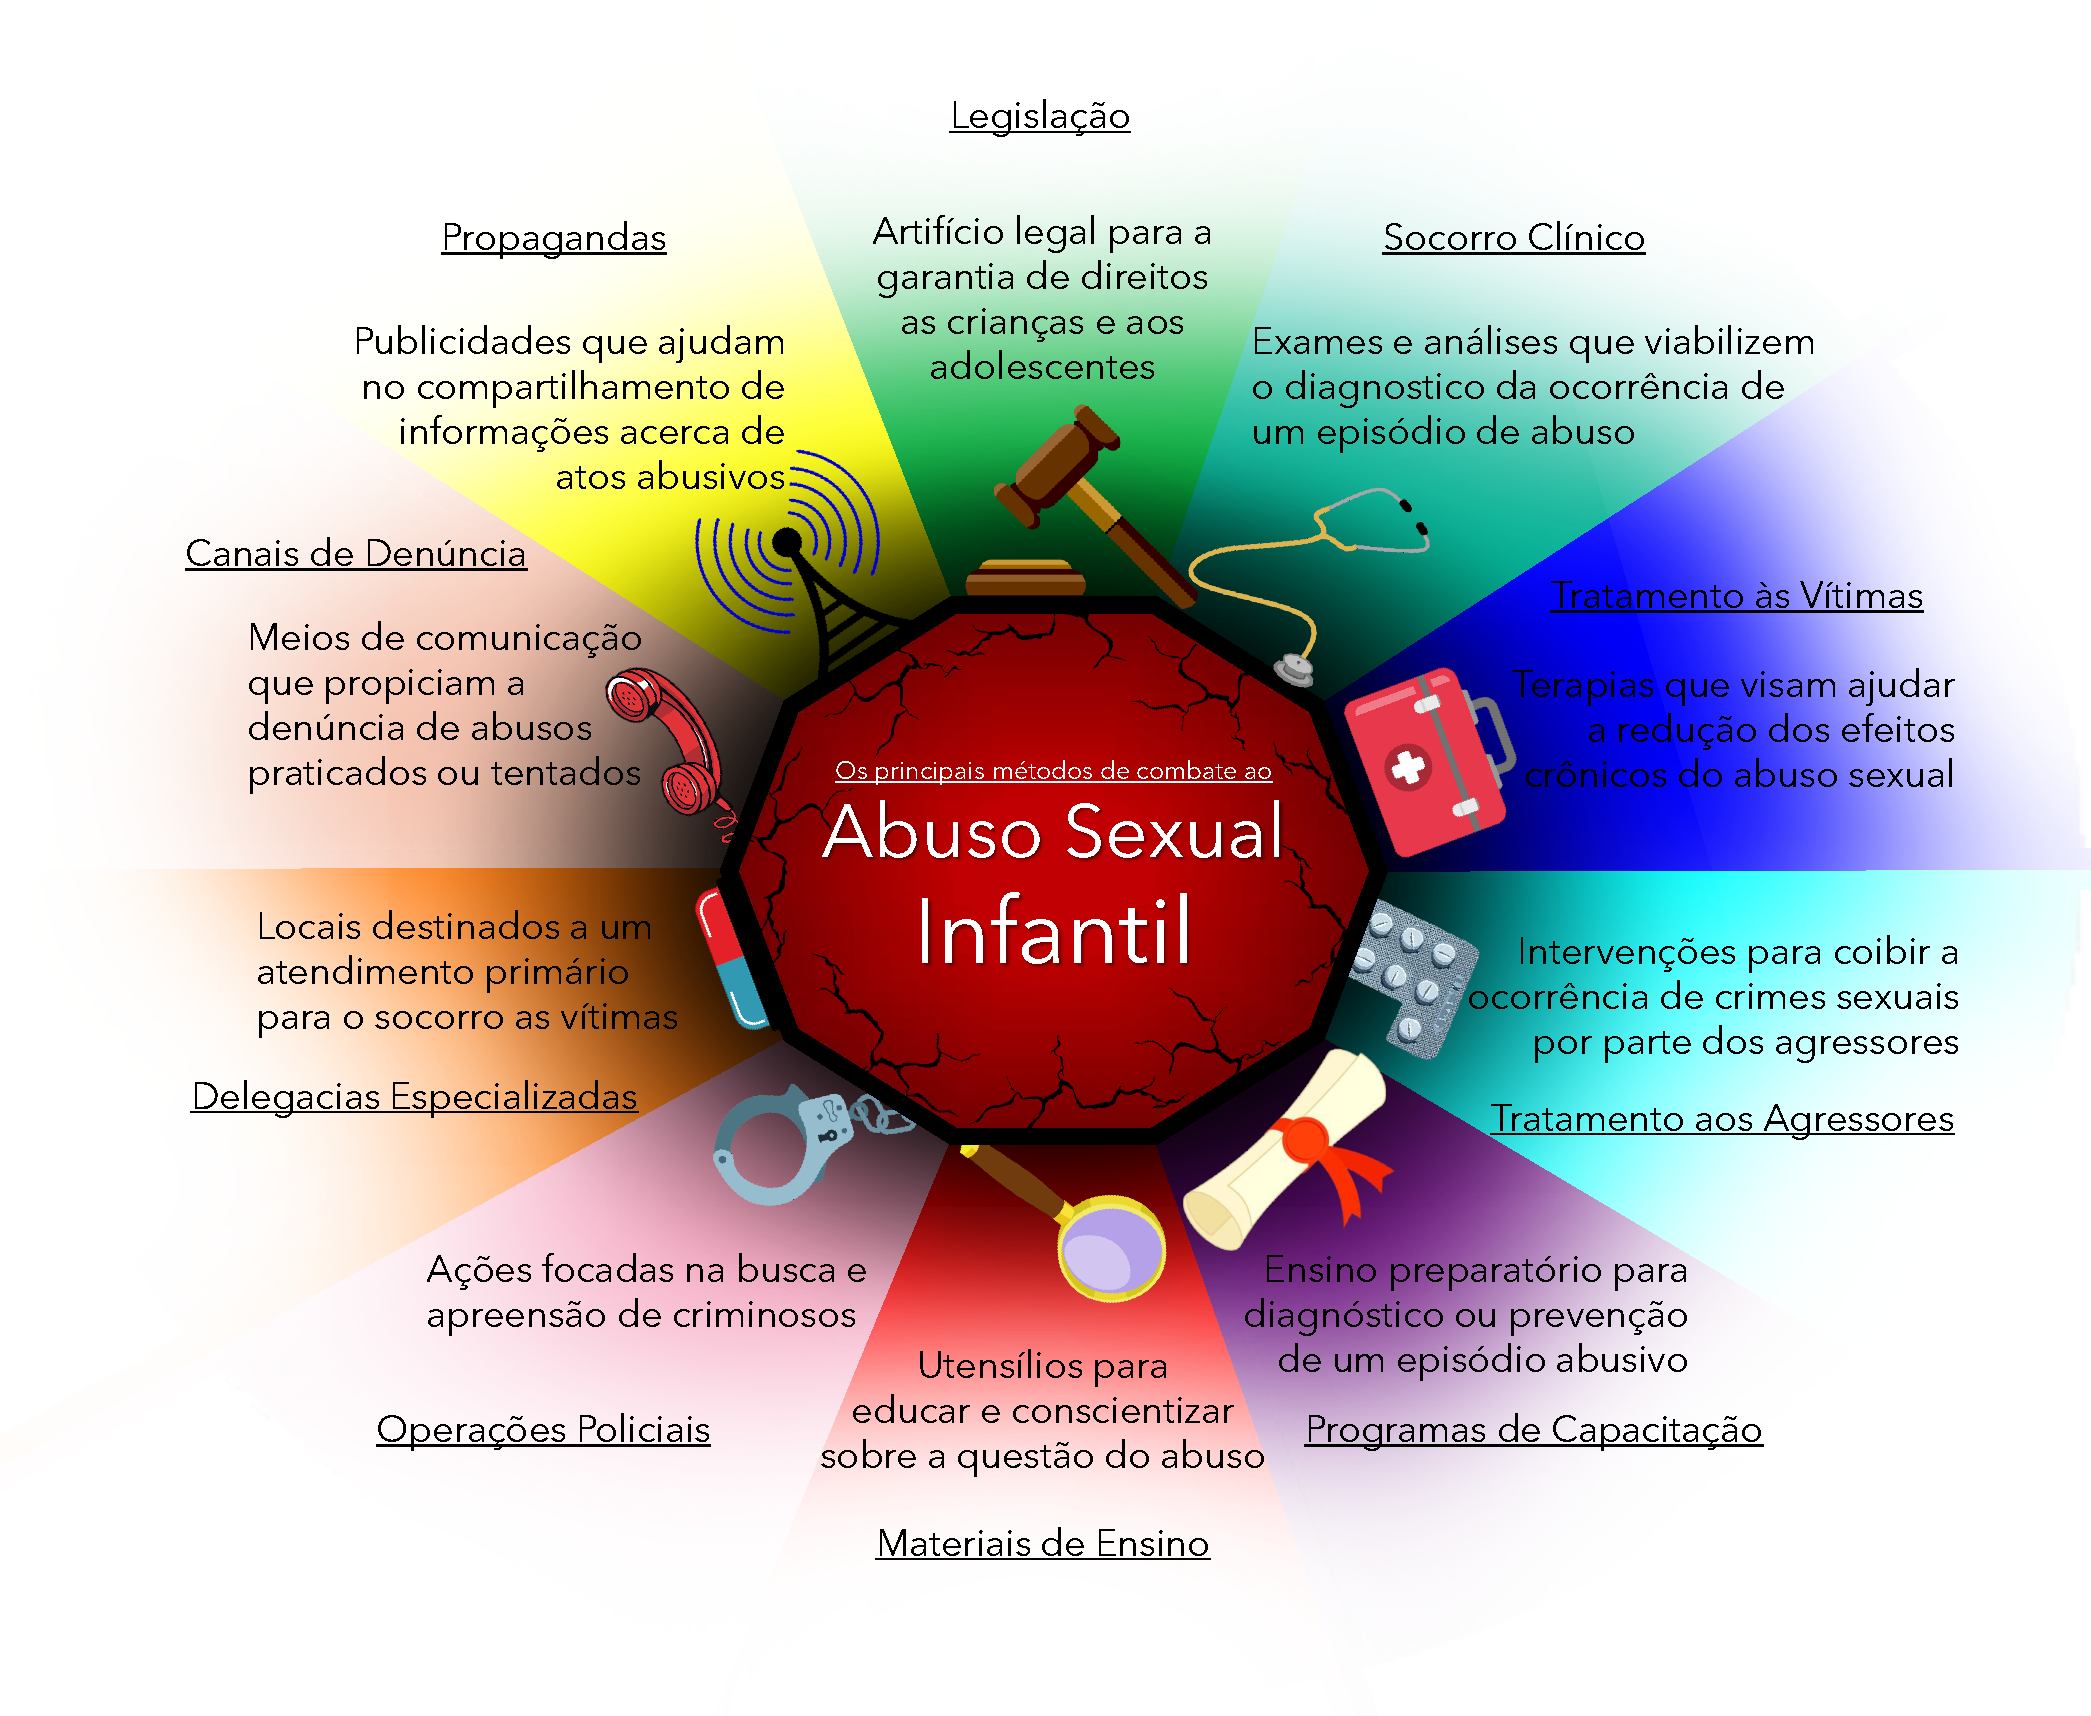
\includegraphics[scale=0.65]{./Figuras/MétodosCombate.pdf}
	\end{adjustwidth}\vspace{-1.5cm}
  \legend{Fonte: Os autores (2020)}

\end{figure}

\newpage



A \autoref{fig:Metodos} ilustra as estratégias de combate a violência sexual infantil apresentadas por este trabalho. No âmbito jurídico foram criadas medidas legislativas (\autoref{sec:regras}), para fornecer artifícios legais de combate ao problema; como a criação de inúmeros meios para a denúncia de criminosos (\autoref{sec:canais}). Para conscientizar as pessoas de seus direitos e dos meios de denúncia, surgiram as propagandas (\autoref{sec:propagandas}). Aos já molestados, medidas surgiram em resposta, voltadas ou ao diagnóstico clínico (\autoref{sec:hospital}) ou ao tratamento das vítimas (\autoref{sec:centros}). Na esfera policial foram criadas as delegacias de atendimento (\autoref{sec:dp}) e as operações policiais (\autoref{sec:op}) que acabam por fornecerem uma resposta de combate direto ao problema. Para os infratores, surgiram iniciativas voltados ao seu tratamento  (\autoref{sec:infratores}). Por fim, no aspecto socioeducativo foram criados programas de capacitação (\autoref{sec:programas}), os quais podem ser complementados por materiais de ensino (\autoref{sec:materiais}), proporcionando assim, um sistema educativo sólido para a conscientização das pessoas sobre o problema. 

\vspace{-0.35cm}

A violência sexual infantil é um grave problema presente na sociedade. Em resposta a este problema sugiram inúmeras medidas nas mais diversas áreas. Por tal razão, este é o tipo de crime que não pode ser abordado numa perspectiva individual, mas sim, abordado em um contexto interdisciplinar e intersetorial \cite{maria2010papel, pinto2017avaliaccao}. %O problema da violência sexual infantil atinge inúmeras áreas, por tal razão o combate a este problema não pode vir apenas de uma área, mas sim de várias as esferas atingidas. 
É importante que as esferas de combate ao problema da violência sexual infantil estejam em sincronia para maximizar os resultados positivos de todas as estratégias. Além disso, para as estratégias preventivas, é crucial que envolvam de maneira ativa, crianças, pais
e professores para atingirem, com sucesso, seus objetivos \cite{dip2016advancing}. 

%[É IMPORTANTE ENVOLVER TODO MUNDO CONTRA O ABUSO]
%``It is important that CSA prevention programmes actively involve children, parents, teachers, officials, key organisations and the wider community''  \cite{dip2016advancing}


%Destaca-se ``importante  destacar  que  a  prevenção  na  área  deve  sempre  envolver  um trabalho interdisciplinar e intersetorial, estimulando a parceria entre os vários segmentos e instituições   sociais,   como   Saúde,   Educação,   Justiça'' \cite{pinto2017avaliaccao}
%``A grande maioria dos investigadores na área tem como consenso a premissa de que este é o tipo de crime que não pode ser abordado numa perspectiva individual, as medidas para o eliminar ou reduzir têm de ser de âmbito comunitário e numa perspectiva macro.''\cite{maria2010papel}

\vspace{-0.35cm}

As estratégias elencadas por esse Capítulo não representam a totalidade de estratégias existentes nesse cenário de combate a violência sexual infantil. Soluções muito abrangentes ou soluções muito vagas não foram apresentadas neste trabalho. No campo das soluções muito abrangentes estão as organizações e fundações de apoio e amparo as crianças. %Há uma variação muito grande de órgãos focados na ajuda e no apoio a crianças vítimas de violência, cada qual com sua própria estrutural operacional e suas próprias métodos de enfrentamento ao problema.
A ausência de uma estrutura padronizada que unisse essas organizações, impossibilitou sua apresentação por este trabalho. No campo das soluções muito vagas é possível citar a dicção. O ensino do vocabulário verbal permite que indivíduos possam se manifestar e se comunicar, sem isso o processo de denúncia torna-se praticamente ineficaz. Embora a comunicação seja uma ferramenta fundamental para o combate da violência infantil, esse tipo de estratégia não foi contemplada pelo presente estudo devido a sua condição peculiar. 


%no intuito de eliminar este mau que assola milhares de crianças todos os anos. As estratégias de combate e enfrentamento ao abuso sexual infantil. Destacase, que estas foram as abordagem encontradas na literatura pesquisada, outras formas de combate Existem outras formas, como dar telefone para as crianças, ensinar ela a falar (pq se ela não sabe se comunicar então é mais difícil saber do abuso), etc. ----Mas o problema é que essa outras formas são genéricas demais, por tal razão não foram abordadas.


\vspace{-0.35cm}

As estratégias de combate a violência sexual infantil podem ser agrupadas de inúmeras formas. Não há registros na literatura especializada que apontem para um agrupamento único e consolidado de estratégias. Todavia, existem  agrupamentos diferentes do apresentado neste trabalho, constituídos inclusive, por estratégias aqui não listadas. Para uma melhor compreensão da temática tratada por esta pesquisa; a leitura desses agrupamentos e compilados de estratégias é mais do que recomendada: \citeonline{tomison2000preventing}, \citeonline{sanderson2004child}, \citeonline{finkelhor2009prevention} e \citeonline{inspire2016seven}.





%Interest in the prevention of child sexual abuse has culminated in a diversity of initiatives implemented nationally and internationally (Finkelhor, 2009; Sanderson, 2004; Tomison Pool, 2000).













%[Sete Estratégias para Pôr Fim à Violência Contra Crianças] não é bem sobre o abuso, mas acho que pode ser util: %https://apps.who.int/iris/bitstream/handle/10665/207717/9789241565356-por.pdf?ua=1




 %\begin{enumerate}
  %\item \cite{mendelson2015parent}

  %\item .[Justice System Restrictions] = ???????????????????

  %\item .[Advocacy and Media Campaigns] = Campanhas governamentais (Darkness to Light, Stop It Now! e Prevention Project Dunkelfeld)

  %\item .[Youth-Serving Organizations] => código de conduta????

  %\item .[School-Based Programs] = AULAS (PROERD)

  %\item .[Treatment of Offenders] = Gestão de Infratores

  %\item .[Treatment of Victims] = Tratamento psicológico (centros de tratamento)
  
  %\item PROPOSTA DO ARTIGO [Parent-Focused Prevention] = Treinamento de Pais (TP)
%\end{enumerate}




%http://www.crianca.mppr.mp.br/arquivos/File/publi/sedh/08_2013_pnevsca.pdf [AQUI FALA DE MAIS ESTRATEGIAS]

%Fundo Municipal dos Direitos da Criança e do Adolescente%http://www.crianca.mppr.mp.br/arquivos/File/publi/abrinq/ppac_fmdca_fundos_guia_passo_a_passo_abrinq_2015



%É importante lembrar que existe diferença entre ``distinção entre ações governamentais voltadas ao enfrentamento da exploração sexual e ações voltadas à prevenção do abuso sexual.''  \cite{caccia2014conselheiros}

%Formas de combate a violência sexual (\textbf{PROGRAMAS [AULAS], EXAMES CLINICOS, OBSERVAÇÕES NO COMPORTAMENTO}):

%\begin{itemize}
 % \item Criança denuncia avô por abuso após aula sobre violência sexual no Paraná. \cite{central2019crianca} [\textbf{Proerd}, avó acareciava ela]
  %\item Criança escreve bilhete após palestra em escola de MT e denuncia pai: 'Já fui abusada pelo meu pai, isso pode ser denúncia?' \cite{lidiane2018crianca} [\textbf{Proerd}, pai abusava ela]
  %\item Mãe descobre que filha de 5 anos foi estuprada ao levar menina em pediatra de RO \cite{jonatas2018crianca} [\textbf{Exames de rotina}, medica constatou abuso pelo primo de 13 anos]
  %\item Menina denuncia padrasto por estupro após palestra sobre violência sexual, no ES [\textbf{PROERD?}]
%\end{itemize}

%REVISAR A CITAÇÃO, PELO QUE PARECE, ESSE TIPO DE CITAÇAO VAI COMO NOTA DE RODAPE E NAO NAS REFERENCIAS... Basta dizer: 'Disponível em: <https://oglobo.globo.com/.......'







%--------- programas educacionais nas escola (estrategia 2)

%https://g1.globo.com/mt/mato-grosso/noticia/2018/09/18/crianca-escreve-bilhete-apos-palestra-em-escola-de-mt-e-denuncia-pai-ja-fui-abusada-pelo-meu-pai-isso-pode-ser-denuncia.ghtml



%Essa artigo fala que o imperador romano Tibério tinha relações com crianças. E também comenta sobre a primeira monografia na área 'Étude médico-légale sur les sevices et mauvais traitements exercés sur des enfants' de Ambroise Tardieu lembrando que antes disso o médico já tinha outros escritos sobre o assunto. \cite{aded2006abuso}

%-------------------- 












%Participação ativa. Programas que incentivam a participação ativa de crianças (por exemplo, dramatizações) são mais eficazes do que aqueles que usam métodos passivos (por exemplo, conceitos de ensino, discussão) ou não participação (por exemplo, filmes, vídeos ou estudo individual de materiais escritos). [AQUI FALA DE ALGUNS FRAQUEZAS DOS PROGRAMAS]  https://www.researchgate.net/publication/242766154_Child-focused_sexual_abuse_prevention_programs_How_effective_are_they_in_preventing_child_abuse



%[\textbf{TEORIA DA MUDANÇA!!!!!!}]

%``Serious Games is an umbrella term used to encompass digital games designed for a purpose beyond entertainment''\cite{dip2016advancing}



\chapter{Trabalhos Relacionados}\label{ssec:JS}

Jogos sérios são utilizados no processo ensino-pedagógico desde o início da década de 1970. A partir desta década, diversos estudos foram conduzidos de modo a identificar os reais impactos que tais jogos tinham no ensino infantil e juvenil \cite{stieler2016paper}. Ao longo dos anos, cientistas e pesquisadores concluíram que a utilização de jogos em sala de aula desencadeava um aumento expressivo no desempenho escolar dos estudantes \cite{wentzel1998social}. O aumento se acentuava mais nas disciplinas relacionadas, de alguma forma, aos conteúdos ministrados pelo jogo. A utilização de jogos em sala de aula é capaz de amplificar os efeitos da aprendizagem escolar \cite{jones2020serious}. Contudo, mesmo com os jogos apresentando resultados positivos na aprendizagem infantil, jogos sérios ainda apresentam baixas taxas de uso no ensino didático das crianças e dos adolescentes. 

A baixa adoção dos jogos no ambiente escolar pode assumir três causas. A primeira está relacionada com a inexistência de jogos apropriados a uma determinada disciplina. A segunda está ligada com a inaptidão de alguns professores em incorporar os jogos a seus planos de ensino. E a terceira está associada com a falta de equipamentos apropriados nas escolas \cite{dip2016advancing}. Estes fatores acabam por dificultar a adoção de jogos no processo de ensino. Este fato poderia explicar o baixo número de jogos sérios voltados a prevenção da violência sexual infantil, retornados durante a execução da etapa bibliográfica deste trabalho. 

Ao se tratar de jogos voltados para prevenção da violência sexual infantil, a literatura pesquisada revela uma quantidade simplória de jogos relacionados a essa temática. Desta quantidade, poucos são os jogos que foram validados por um processo rigoroso e que apresenta resultados positivos relacionados a aprendizagem infantil \cite{jones2010being}. O atual capítulo dá ênfase aos três jogos de maior relevância identificados de acordo com a literatura pesquisada. Deste modo, a \autoref{sssec:Being} aborda sobre o jogo \textit{Being Safety Smart}, a \autoref{sssec:Orbit} discorre sobre o jogo \textit{Orbit Rescue} e a \autoref{sssec:CeS} discute sobre o jogo \textit{Cool and Safe}. A \autoref{sssec:outros} realiza um comparativo entre os jogos apresentados neste capítulo.


%A \autoref{sssec:outros} realiza um comparativo entre os jogos apresentados neste capítulo, além de apresentar brevemente outros jogos retornados no processo de busca literária, porém que não passaram por um processo de validação com crianças. Em adendo, enfatiza-se que soluções empresariais baseadas em jogos não são contempladas pelo atual trabalho acadêmico, seja pelo fato dos jogos não terem sido devidamente validados ou seja por não estarem devidamente publicadas em acervos acadêmicos.





%Muito poucos foram avaliados rigorosamente e podem evidenciar ganhos positivos no aprendizado infantil e no suporte comportamental \cite{jones2010being} essa seção destaca os três jogos mais bem documentados encontrados na literatura pesquisa, demais jogos são tratando em menores detalhes na seção seguinte.

%os jogos sérios são eficazes para aumentar os efeitos da aprendizagem, levando a um desenvolvimento funcional positivo \cite{jones2020serious}



%O atual trabalho realizou uma busca por jogos com temática preventiva ao abuso sexual infantil que tenham tido aplicação no contexto escolar. Somente dois jogos que obedeciam este critério foram encontrados no processo de pesquisa. Sendo assim, a \autoref{sssec:Being} irá abordar soibre o jogo \textit{Being Safety Smart}, a \autoref{sssec:Orbit} irá abordar sobre o jogo \textit{Orbit}, enquanto a \autoref{sssec:CeS} irá abordar sobre o jogo \textit{Cool \& Safe}. 






%o uso da cultura popular no ensino pode aumentar os níveis de motivação e compreensão dos alunos \cite{cheung2001use, chik2011learner, duncan2004your, giroux1988schooling}


%https://ap-st01.ext.exlibrisgroup.com/61USC_INST/upload/1605206133717_PDF%20-%20Thesis.pdf?Expires=1605206256&Signature=unRq1Gd6WGKxXJJM0jTo~OyQdLrwGcS1rF~cjUaDj2XI4f8ldD4lb-VUkJMV89UsyH6YeDJMBdVv~JPde6fP4q8xn14EsoxQfdoWl~YMd38yDIovAWkhRm228m4yjrcX7LAMWt-8YmruwRzEcvbMnLgUrmphnO~wSuPsypAFOmtPzcRvrZ55G-4e-RNc4SrzfhB-gK3LpgH6DD07ZU1Ua07jg9RKyWLIP6HYI-wAizbxbCjFokQUYEh281Jy9uwJkjWD9dlICuhCzftH6KbtXo0bCqlYCUtuPcIbNLKUjygxas9Armwt5CWexm7SvngSM5DR2aHEdN-dt9xJMPLdmw__&Key-Pair-Id=APKAJ72OZCZ36VGVASIA = Advancing the use of Digital Game-Play in Primary and Secondary School Classrooms to Establish Supportive and Engaging Classroom Learning Environments

%https://www.finersistemas.com/atenaeditora/index.php/admin/api/artigoPDF/26296

%https://www.udesc.br/arquivos/cct/id_cpmenu/1024/disserta_ao_completa_15532596804969_1024.pdf

%https://pdfs.semanticscholar.org/1d76/ee8a9260238ff962409c88018ddeba80363d.pdf

%https://br-ie.org/pub/index.php/sbie/article/view/8163/5849

%https://sci-hub.do/10.1016/j.chiabu.2020.104569

%https://sci-hub.do/10.1080/10538712.2019.1663969

%https://www.researchgate.net/publication/259932747_The_Teachers%27_Role_in_Child_Sexual_Abuse_Prevention_Programs_Implications_for_Teacher_Education

%https://www.researchgate.net/publication/259932746_Serious_games_for_learning_games-_based_child_sexual_abuse_prevention_in_schools


%``Digital games have been used sporadically in classrooms since the 1970s'' (pagina 54) \cite{dip2016advancing}

%``Digital games have been used in classrooms since the 1970s with some of the most successful early educational titles being Oregon Trail and Lemonade Stand (Egenfeld-tNielsen, 2005)''\cite{dip2016advancing}
%[APRENDER FAZENDO!!!!]
%``One of the many benefits of digital games is the facilitation of opportunities to ‘learn through doing’'' \cite{dip2016advancing}

%[esse artigo tem uns graficos legais, mas antigos.. (SEPARAÇÃO POR RELIGIÃO, ESCOLARIDADE)] [declarações ESPONTANEAS OU NAO DAS CRIANÇAS: enfatizando a importancia de questiona-las] PERGUNTAAAAA: será que o jogo deveria questionar a criança?????????? \cite{cardoso2016abuso} ....tem mais coisas interessantes nesse artigo!!!!!!

%``Barriers to using digital games in classrooms include negative societal attitudes towards digital games, teachers not being able to find games that suit their curriculum, teachers not knowing how to incorporate games into their curriculum, not enough time in the school day and inadequate access to appropriate hardware and software'' [BARREIRAS NO USO DE JOGOS, mas o artigo da algumas soluções] \cite{dip2016advancing}

%``In this paper, we will use the term immersive digital games (IDGs) to refer to digital games that are more likely to involve the player in deep exploration and have them participate in activities that vary greatly from didactic instruction'' \cite{dip2016advancing}

%A systematic review of international education and training programmes for CSA prevention in schools was conducted to identify best practice in CSA prevention and appropriate key messages suitable for children. To minimise bias, protocols were developed with criteria for a ‘systematic review’ (MacDonald 2000). Following Evans and Benefield (2001) framework, clear and explicit steps were taken in a systematic search to address the general research question. =Serious games for learning: games- based child sexual abuse prevention in schools
%REVISAO REVISAO REVISAO

\section{Being Safety Smart}\label{sssec:Being}

%The most vulnerable age for sexual abuse is between 7 and 13 years [4]

\textit{Being Safety Smart}\footnote{\textit{Being Safety Smart} é um jogo  da Universidade de Sunshine Coast lançado em fevereiro de 2009. No momento da redação deste trabalho o portal do jogo encontra-se fora do ar. No entanto a página virtual do jogo ainda pode ser acessada por meio de bibliotecas digitais voltadas a manter um acervo de páginas públicas do mundo virtual. Para ter acesso ao jogo basta recorrer a uma desta bibliotecas digitais e pesquisar pelo antigo portal do jogo: \url{http://www.beingsafetysmart.com.au}.} é um jogo virtual projetado para combater o sequestro e a violência sexual de crianças. O jogo é voltado para crianças de seis a oito anos. O jogo almeja capacitar as crianças de modo que elas respondam adequadamente ao problema da violência sexual infantil \cite{jones2008online}. Para isso, o jogo aborda  o problema do abuso e do sequestro de crianças por meio de oito níveis distintos voltados para o fortalecimento da segurança pessoal das crianças. Os oito níveis podem ser visualizados na tela principal do jogo, ilustrada na \autoref{fig:BSS1}. 

%para prevenir a violência sexual infantil e combater o sequestro de crianças na Austrália. O jogo é voltado para crianças de seis a oito anos de idade e tem como ideia principal a conscientização das crianças sobre sua segunrança pessoal, ajudando-as e capacitando-as a reagir adequadamente ao problema \cite{jones2008online}.

\begin{figure}[htb]
  %\vspace{-0.5cm}
	\caption{\label{fig:BSS1}Tela Principal do jogo \textit{Being Safety Smart}.}
  \begin{center}\vspace{-0.3cm}
    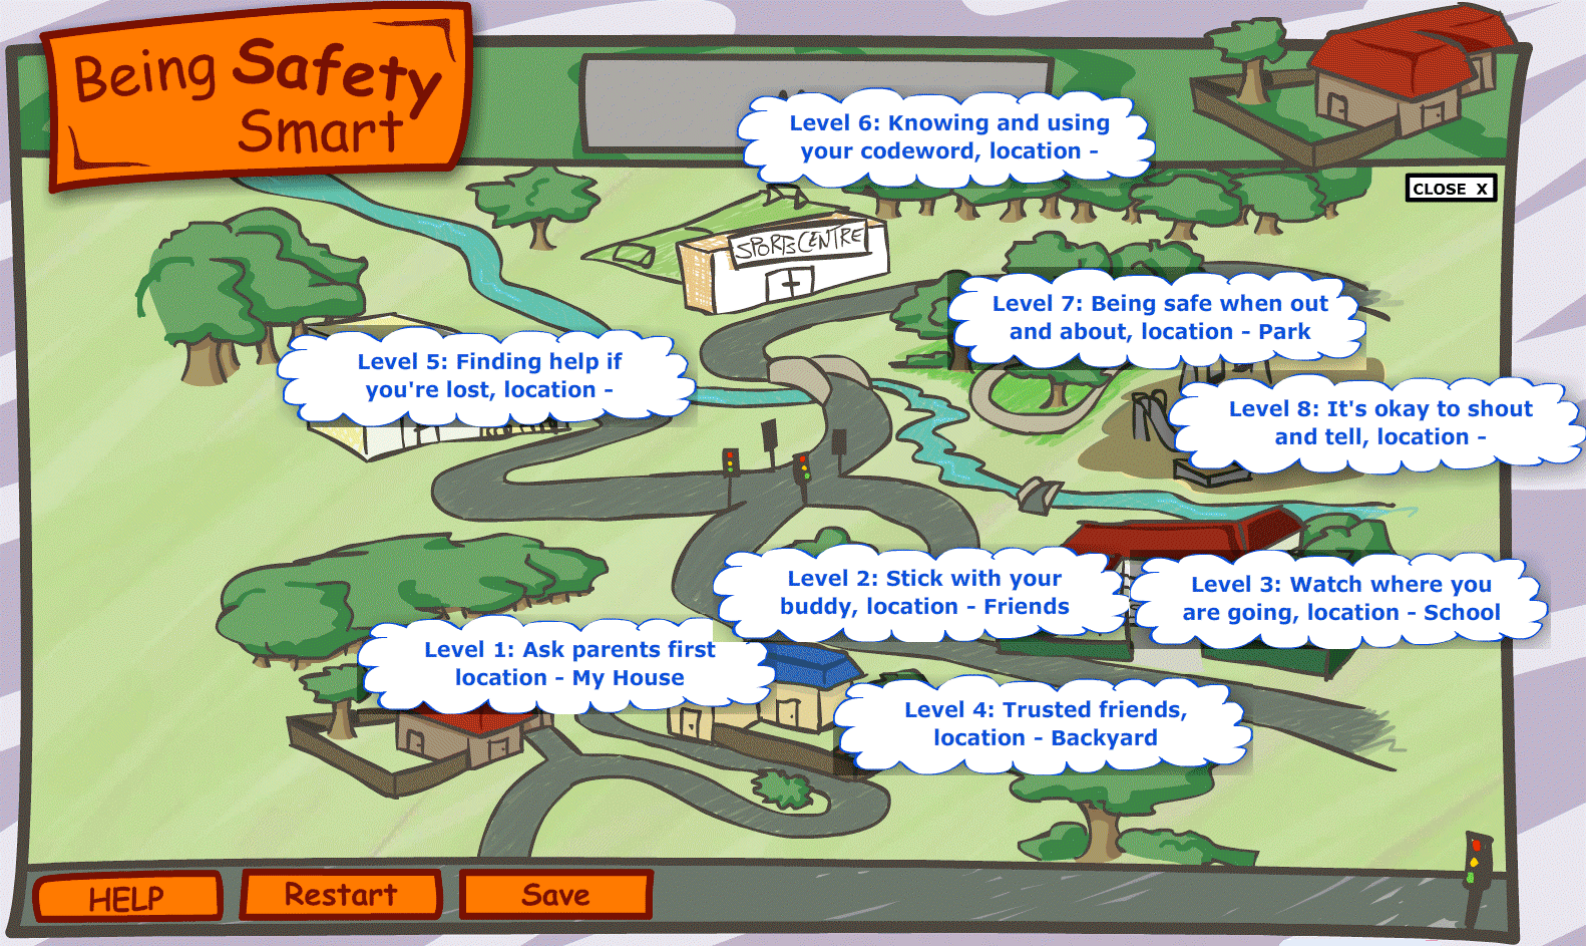
\includegraphics[width=\linewidth]{./Figuras/BSS/B1.png}
	\end{center}\vspace{-0.5cm}
  \legend{Fonte: \citeonline[p. 3]{jones2008online}}

\end{figure}

A \autoref{fig:BSS1} apresenta a tela principal do jogo \textit{Being Safety Smart}. Oito níveis com diferentes conteúdos didáticos são mostrados nesta tela. Cada nível assume a representação de um ambiente do mundo real. O ambiente representado se relaciona de alguma forma com os assuntos a serem ministrados neste nível. O primeiro nível é ministrado em um ambiente virtual que visa representar a casa da criança, o segundo nível a casa dos amigos da criança, o terceiro nível a escola da criança, o quarto nível a vizinhança da criança, o quinto nível um supermercado, o sexto nível uma quadra esportiva, o sétimo nível um parque e o oitavo nível um pátio recreativo.

\begin{wrapfigure}[38]{r}{3.5cm}%pulando 38 linhas
  \vspace{-5pt}
  \caption{\label{fig:NiveisBBS}Níveis.\vspace{5pt}}

  \subfloat[Nível 1\label{fig:1}\vspace{-5pt}]{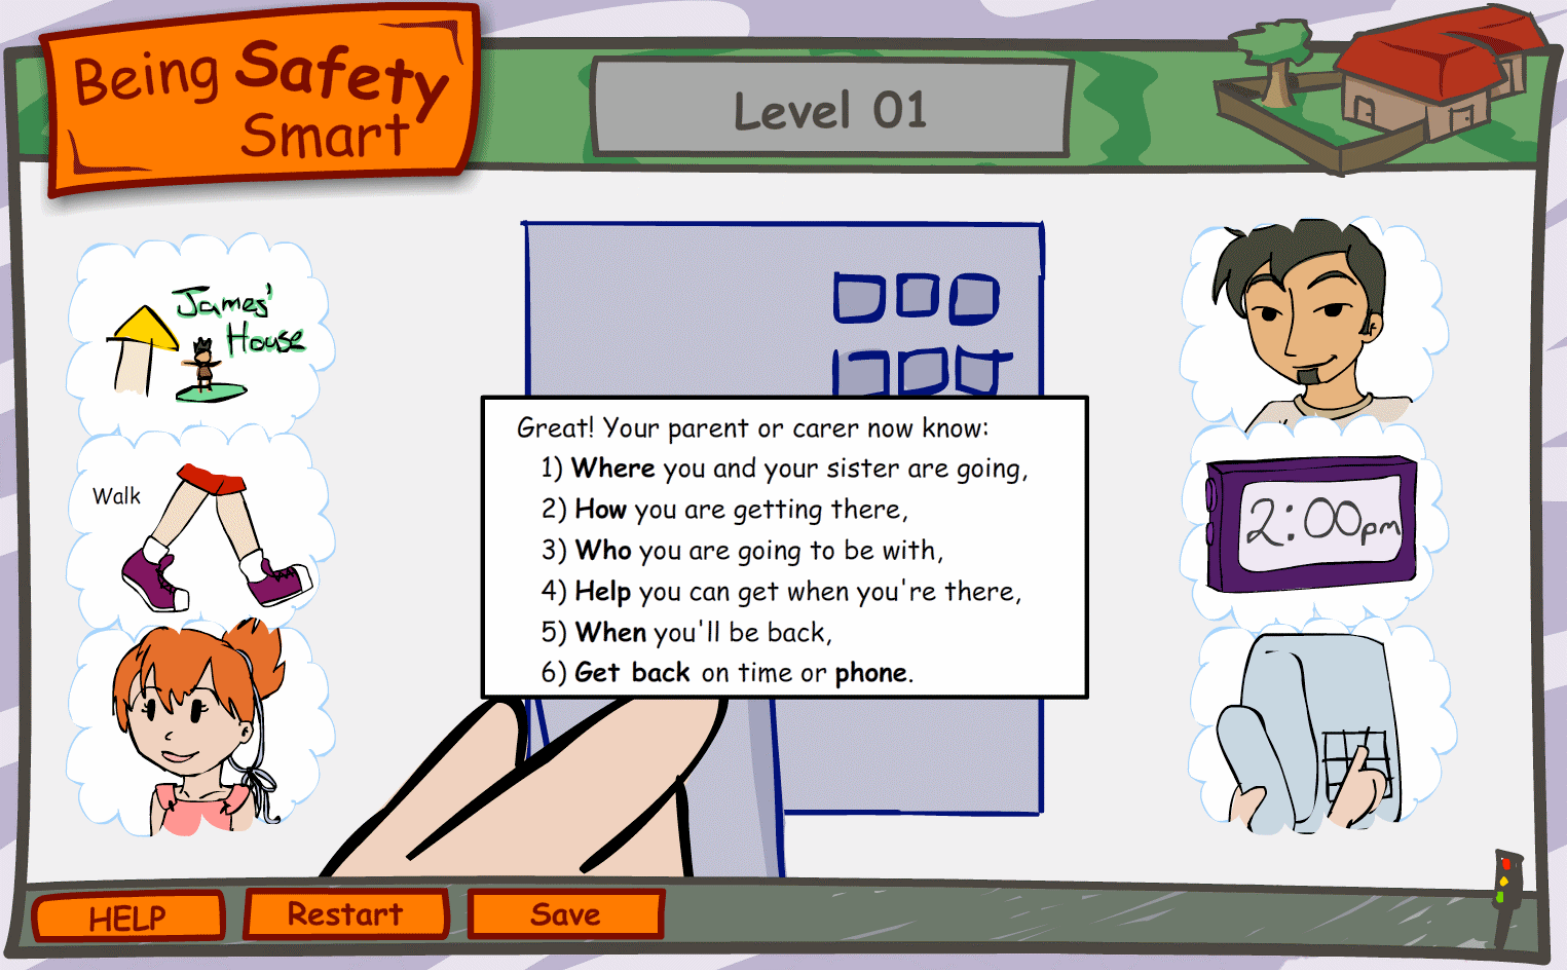
\includegraphics[width=\linewidth]{./Figuras/BSS/B5.png}}\vspace{-3pt}
  \\
  \subfloat[Nível 2\label{fig:2}\vspace{-5pt}]{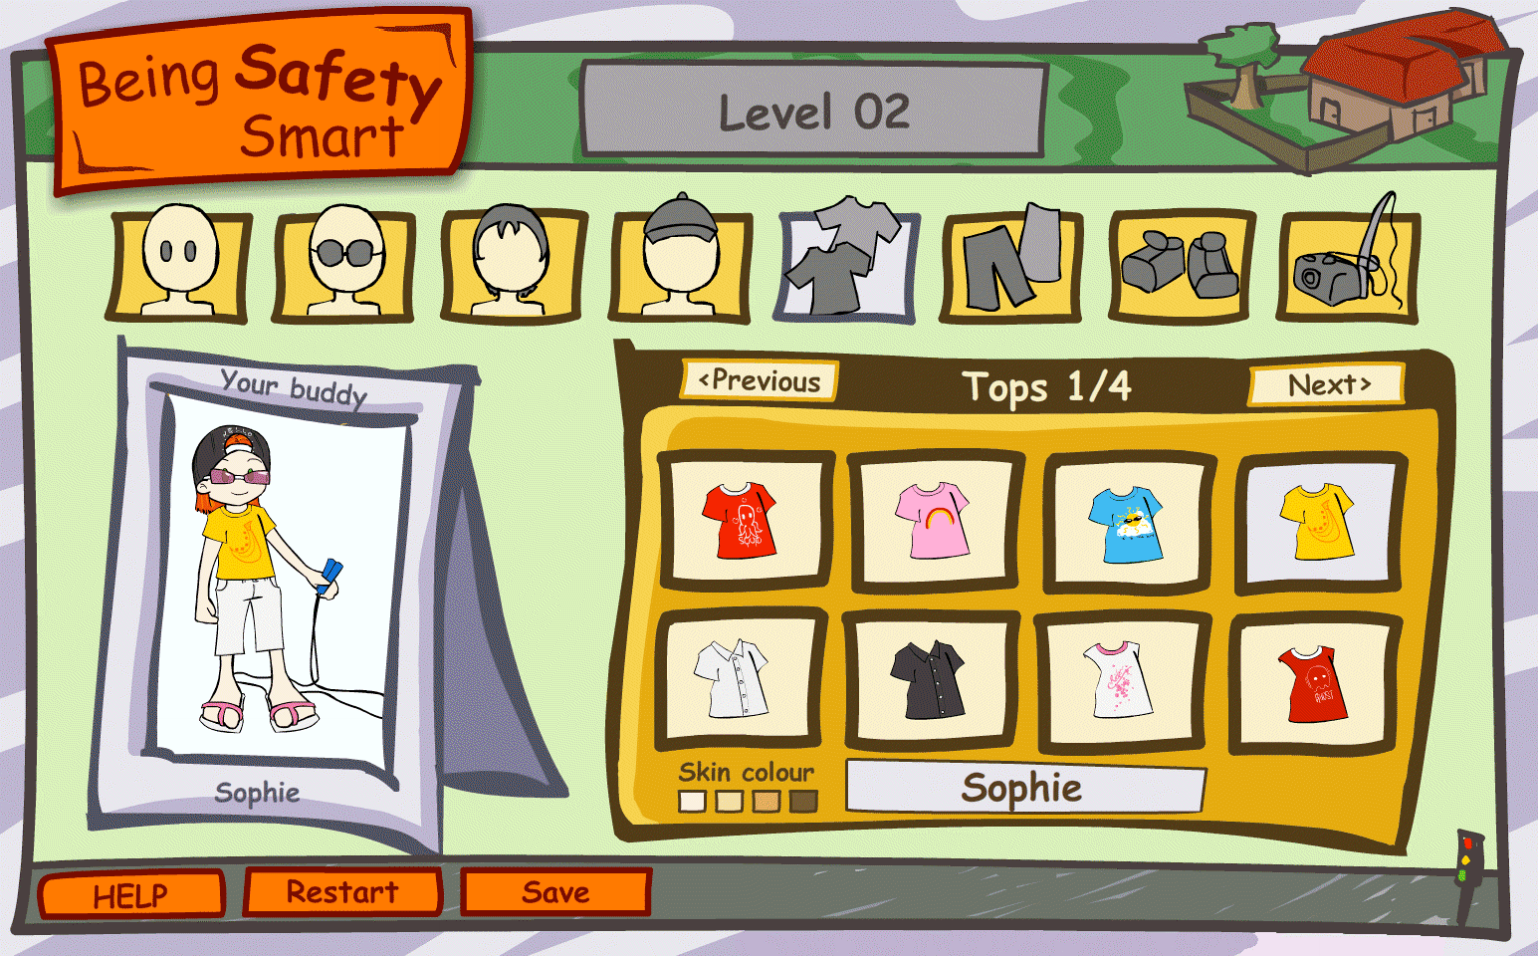
\includegraphics[width=\linewidth]{./Figuras/BSS/B2.png}}\vspace{-3pt}
  \\
  \subfloat[Nível 3\label{fig:3}\vspace{-5pt}]{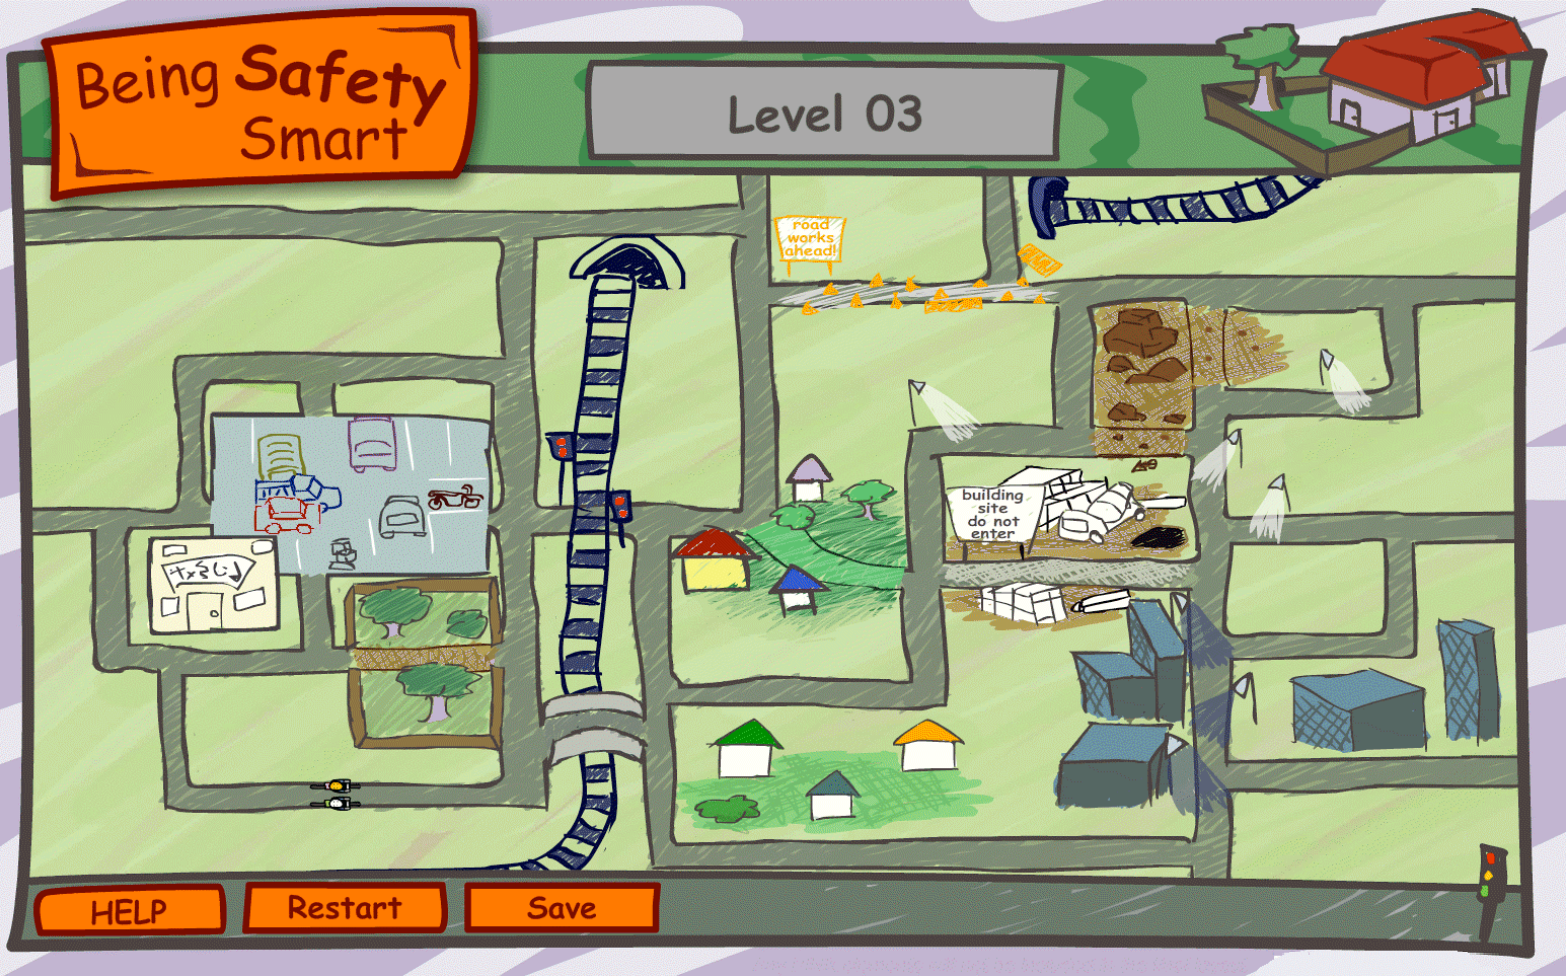
\includegraphics[width=\linewidth]{./Figuras/BSS/B8.png}}\vspace{-3pt}
  \\
  \subfloat[Nível 4\label{fig:4}\vspace{-5pt}]{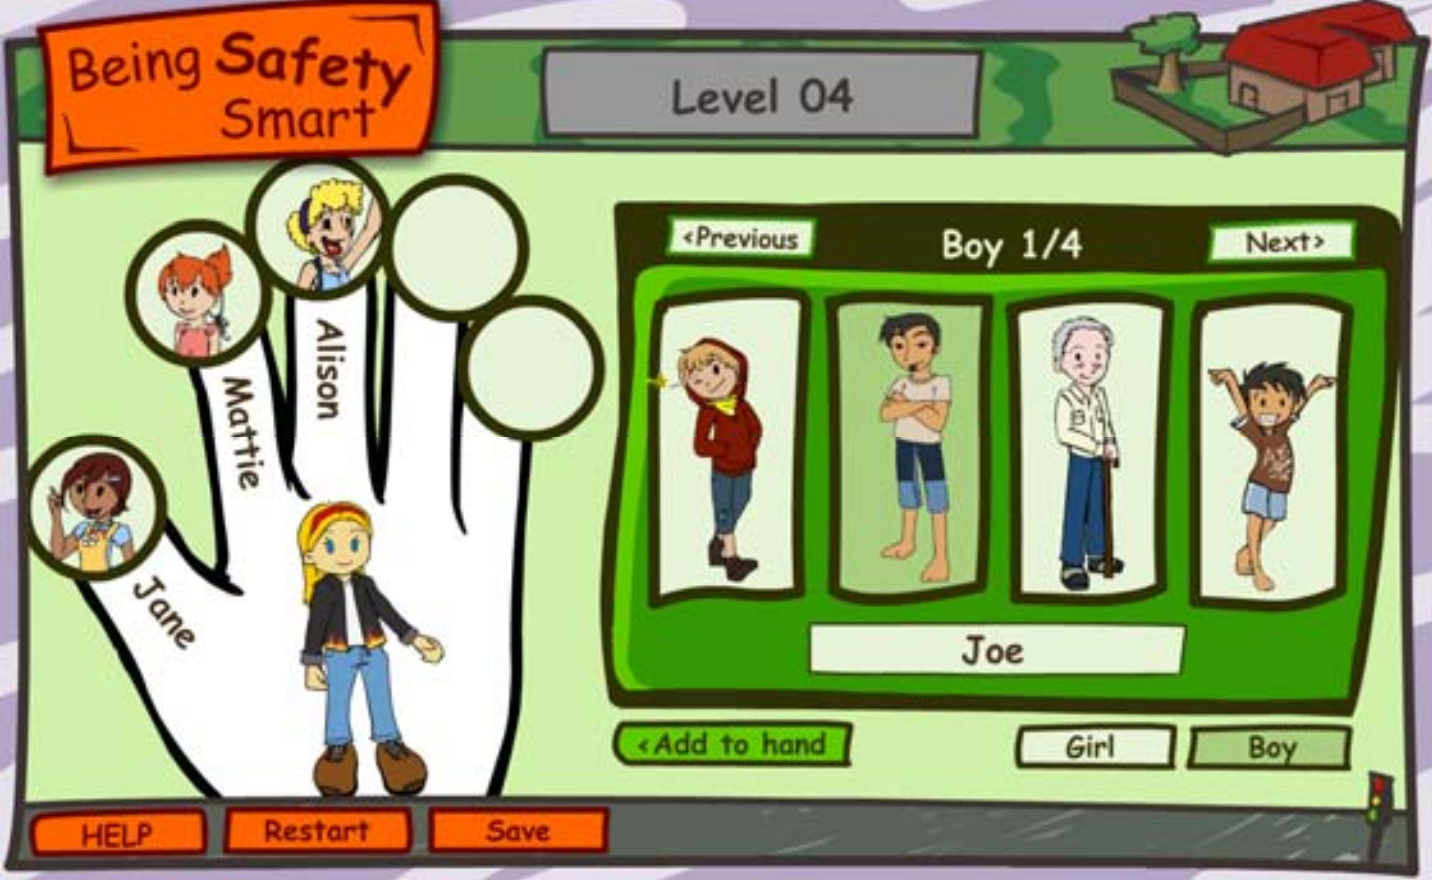
\includegraphics[width=\linewidth]{./Figuras/BSS/B9.png}}\vspace{-3pt}
  \\
  \subfloat[Nível 5\label{fig:5}\vspace{-5pt}]{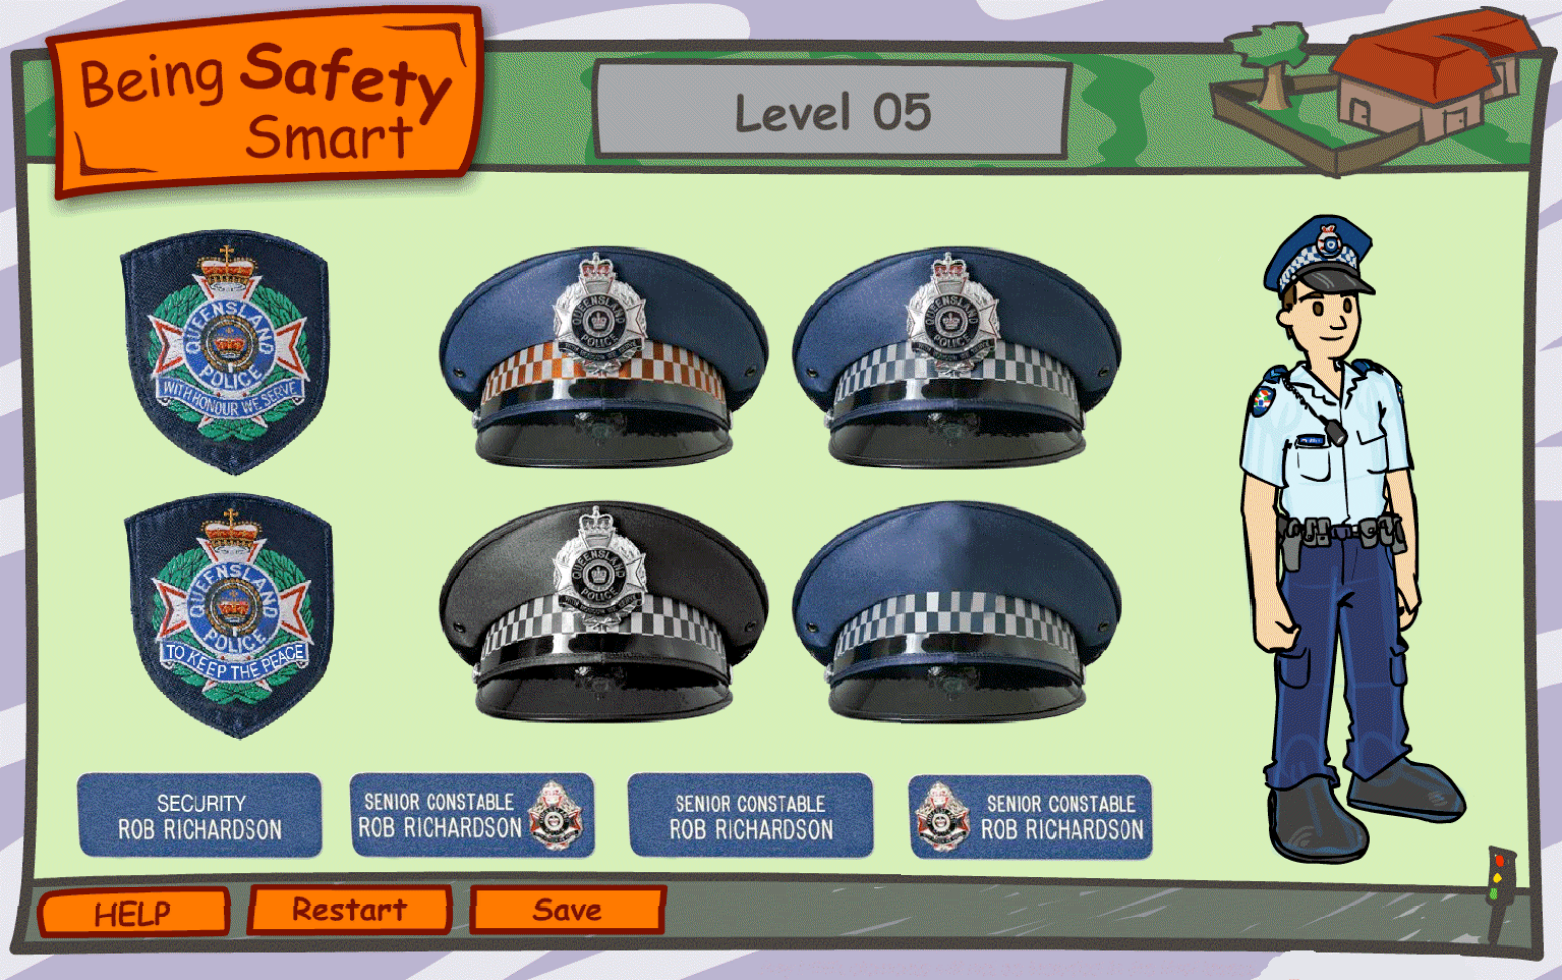
\includegraphics[width=\linewidth]{./Figuras/BSS/B6.png}}\vspace{-3pt}
  \\
  \subfloat[Nível 6\label{fig:6}\vspace{-5pt}]{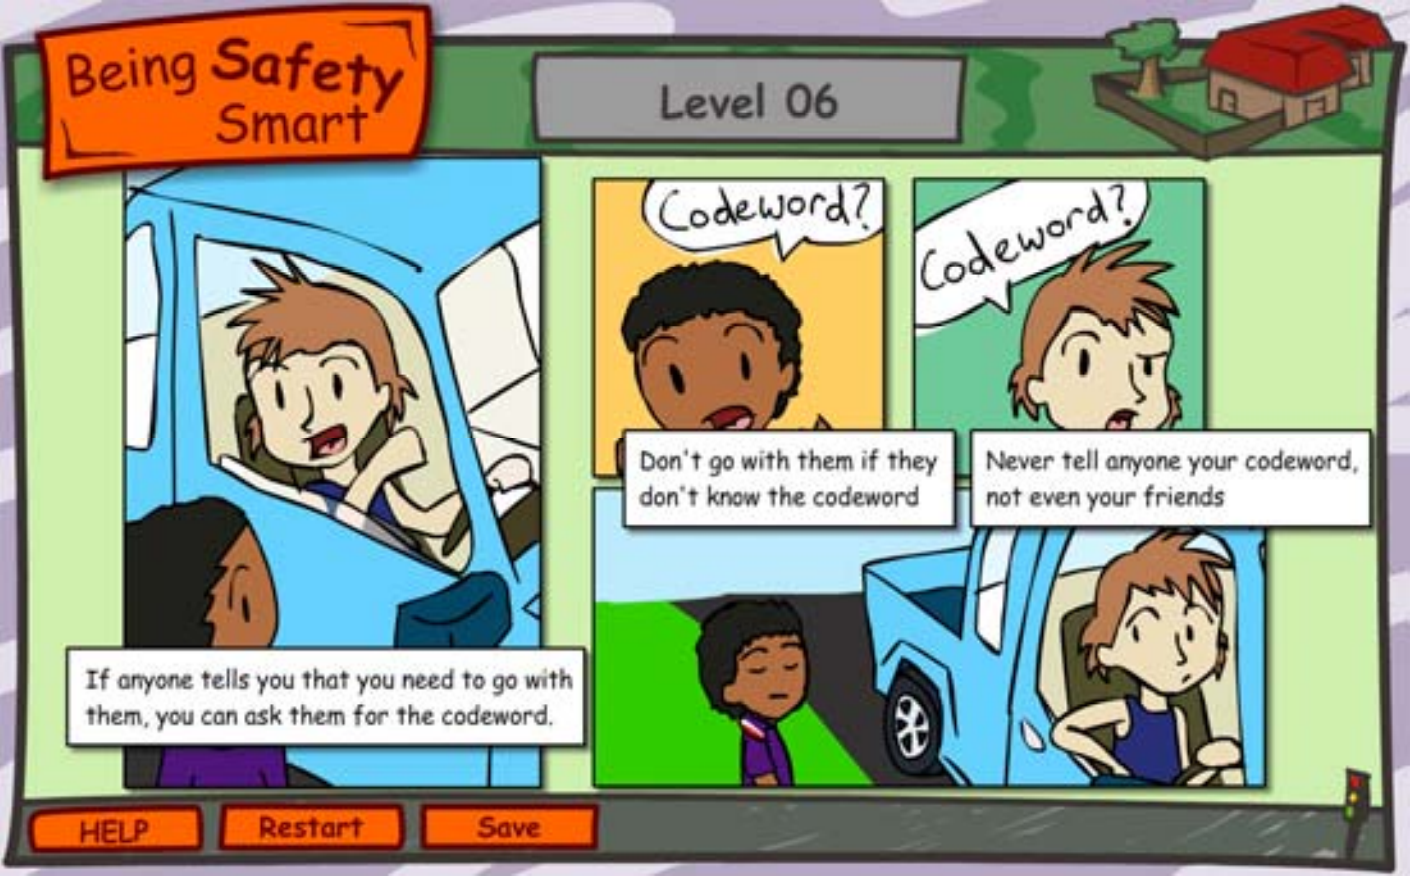
\includegraphics[width=\linewidth]{./Figuras/BSS/B10.png}}\vspace{-3pt}
  \\
  \subfloat[Nível 7\label{fig:7}\vspace{-5pt}]{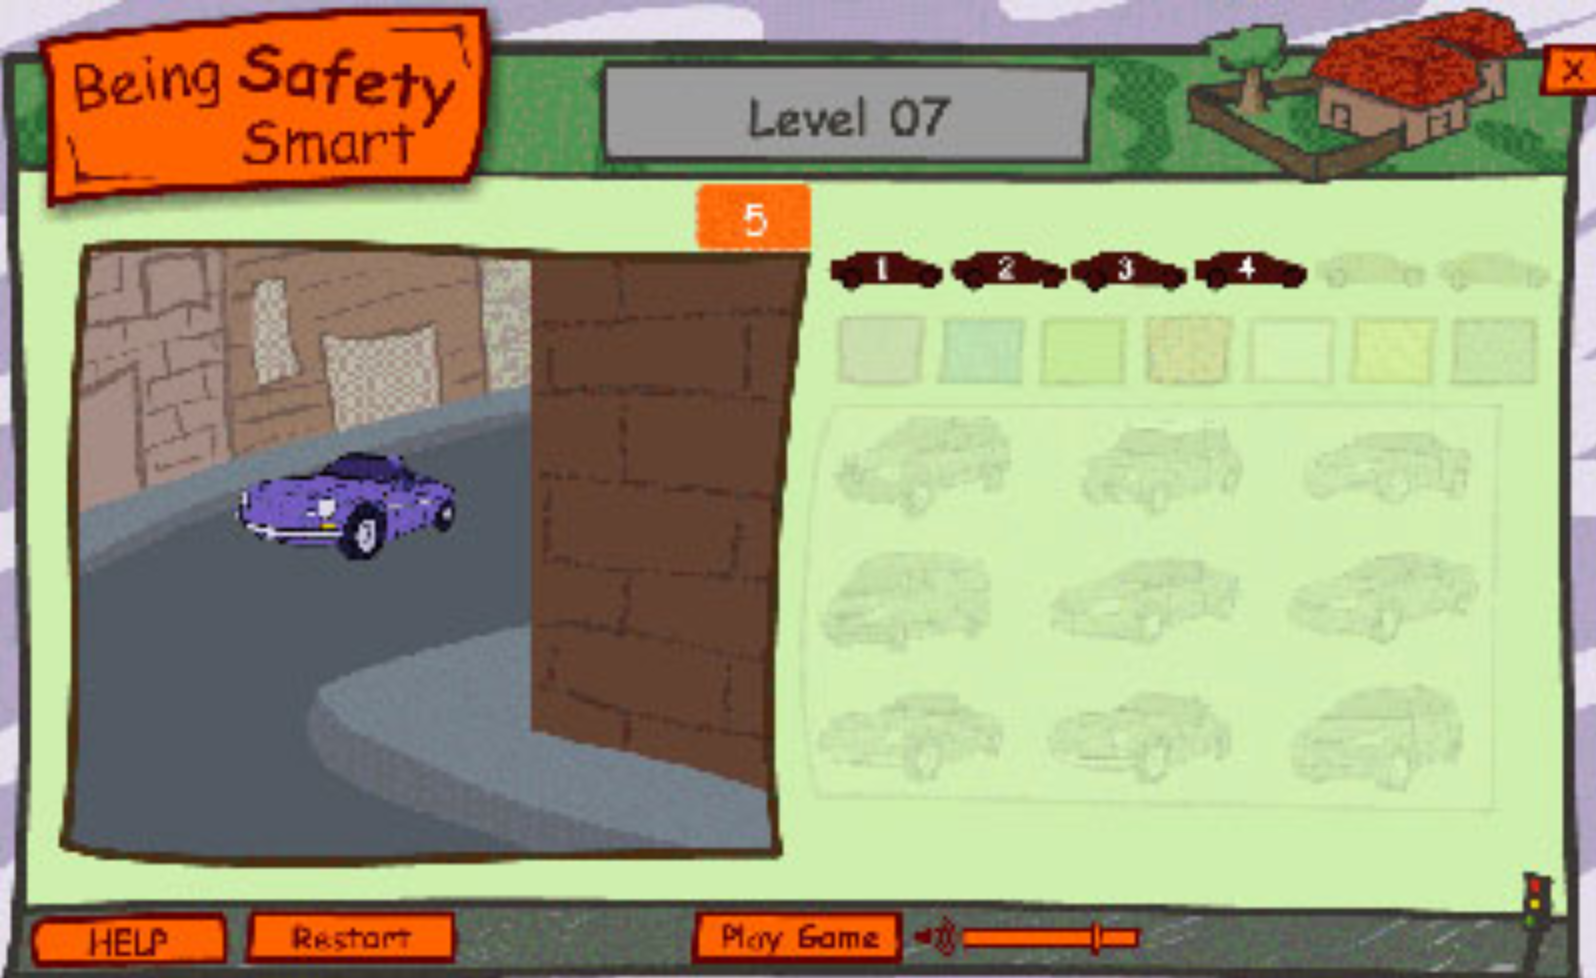
\includegraphics[width=\linewidth]{./Figuras/BSS/B12.png}}\vspace{-3pt}
  \\
  \subfloat[Nível 8\label{fig:8}\vspace{-5pt}]{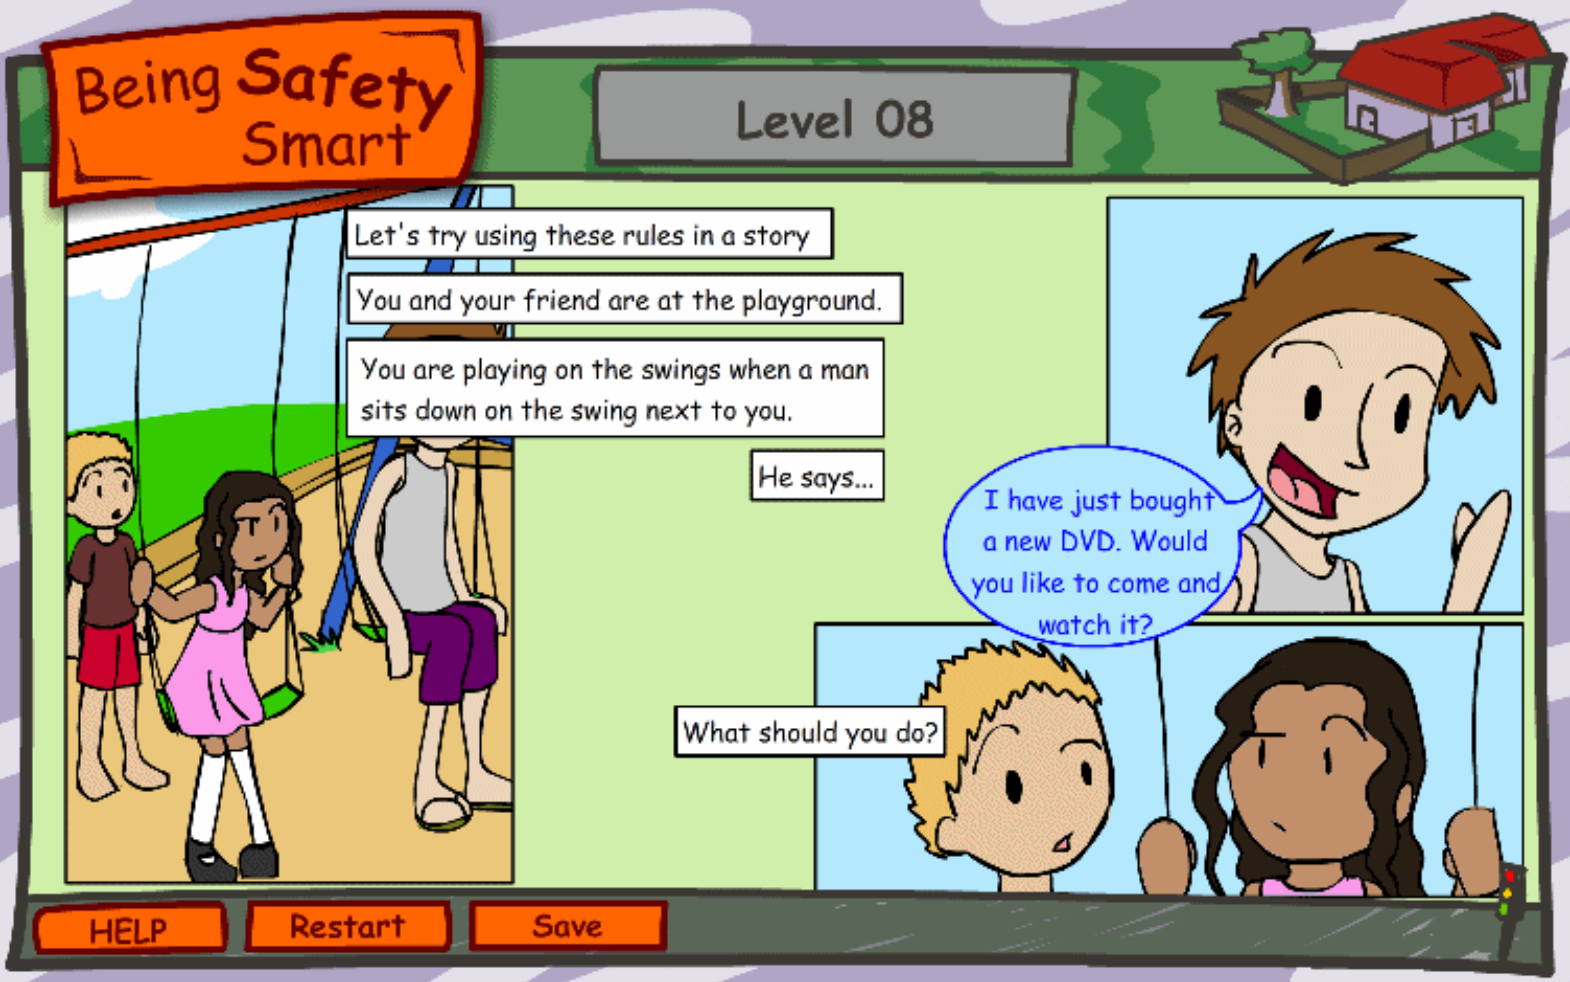
\includegraphics[width=\linewidth]{./Figuras/BSS/B11.png}}
  \vspace{-8pt}
  \legend{Fonte: \citeonline{jones2008online}.}%eu paguei outros nao citados aqui, como fazer a referencia?
  %india (mas não governamental)
\end{wrapfigure}

A numeração dos níveis representa a linearidade imposta pelo jogo ao jogador. O jogo exige um cumprimento linear dos seus níveis, tanto por motivos de enredo, quanto por motivos pedagógicos de ensino. Um jogador só pode acessar os níveis inferiores ao seu progresso no jogo. O jogador precisa esperar que a história do jogo vá destravando, um a um, os níveis superiores. No primeiro nível (Figura \ref{fig:1}) a criança aprende que deve sempre informar aos seus pais (ou responsáveis) os locais aonde vai e com quem vai ao sair de casa com os amigos. No segundo nível (Figura \ref{fig:2}) o jogador é ensinado a nunca andar sozinho sempre que isso for possível. No terceiro nível (Figura \ref{fig:3}) a criança é instruída a caminhar sempre por locais seguros e conhecidos. No quarto nível (Figura \ref{fig:4}) o menor aprende a reconhecer e identificar cinco adultos em quem possa confiar. No quinto nível (Figura \ref{fig:5}) o jogador é ensinado a identificar outras pessoas a quem possa pedir ajuda ou auxílio. No sexto nível (Figura \ref{fig:6}) o menor aprende a identificar pessoas confiáveis através de códigos (e.g. códigos ou \textit{codework} são senhas usadas entre as pessoas para reconhecerem se a outra pessoa é uma pessoa de confiança). No sétimo nível (Figura \ref{fig:7}) o jogador aprende a evitar convites ou favores de estranhos. E no oitavo nível (Figura \ref{fig:8}) o jogo ensina ao jogador a sempre comunicar e contar para pessoas de confiança situações incomuns que tenham acontecido com ela. 

%situações incomuns que acometeram a criança.


%O primeiro nível visa ensinar as crianças a sempre informarem aos seus pais onde estão indo. O segundo nível educa as crianças da necessidade de sempre estar acompanhado e evitar andar sozinho. O terceiro nível tem como foco ensinar as crianças a evitar caminhos desconhecidos e sempre optar por locais seguros. O quarto nível se baseia em educar os menores sobre a necessidade de ter pessoas de confiança em diferentes locais. O quinto nível tem como objetivo auxiliar as crianças de como pedir ajuda e a quem pedir ajuda. O sexto nível ensina as crianças a terem palavras secretas com pessoas de confiança e como usar essas palavras (e.g. palavras secretas ou \textit{codework} são senhas usadas entre as pessoas para reconherem se a outra pessoas é uma pessoa de confiança). O sétimo nível avisa as crianças sobre como interagir com estranho (e.g. evitando caronas de desconhecidos e presentes ou doces de estranhos). O oitavo nível tem como foco ensinar as crianças a não guardarem segredos de coisas ruins que tenham acontecido. Cada nível apresenta uma seção de instrução, uma seção de atividades e um resumo dos conceitos aprendidos. 

%O jogo possui versão em CD-ROM (que não requer internet) e versão para navegadores. Ao acessar o jogo após um breve cadastro a criança é apresentada ao mapa do jogo, no qual oito ambiente compõem o ambiente. O jogo é completamente linear, e o jogador precisa concluir os níveis anteriores para avançar no jogo. A ideia do jogo é que a criança vá construindo na aprendizagem anterior com habilidades, comportamentos e estratégias mais complexos. 

Todos os níveis do jogo \textit{Being Safety Smart} compartilham a mesma arte baseada em quadrinhos infantis. Cada diálogo do jogo é acompanhado por texto escrito e dublagem em língua inglesa. Além disso, os níveis do jogo compartilham a mesma estrutura didática baseada em três conceitos metodológicos de ensino. Inicialmente o jogador é apresentado as instruções de um determinado nível. Posteriormente o jogador é confrontado com uma atividade lúdica interativa. E por fim, o jogador é apresentado a um resumo do nível. Os oito níveis do jogo são projetados para serem ministrados em um ambiente escolar no decorrer de oito semanas. Contudo, nada impede que o jogo seja ofertado em blocos mais curtos ou mais longos de tempo a depender das temáticas já ministradas pela escola \cite{jones2010being}. Em adendo, a literatura revela que 200 escolas já ministraram o jogo \textit{Being Safety Smart} a seus alunos.


%A arte do jogo é feita em comic-style panels O jogo permite a customização do personagem. Begin Safety Smart contém 8 níveis e é projetado para ser entregue ao longo de 8 semanas. Porém a ferramenta pode ser fornecido em um modo de ensino em bloco mais curto ou por um período de tempo mais longo. O jogo apresenta todo seu conteudo na lingua inglesa, tanto textualmente quanto sonoramente. 



%A seção de instrução apresenta as principais mensagens de conscientização sobre segurança infantil para o nível usando janelas e fontes de desenho animado estilo revista, junto com animações dinâmicas de cenários. Todas as informações textuais também são apresentadas como uma trilha de áudio falada por crianças da mesma idade. A seção de atividades / jogos reitera a mensagem apresentada na seção de instrução e testa a compreensão da criança por meio de jogos e dramatizações interativas. Existem três estilos principais de atividades: i) escolha entre três opções de ‘o que fazer a seguir’, consulte a Figura 8; ii) seleção de itens corretos da exibição de vários itens; iii) e jogos interativos. A criança recebe informações adicionais para cada seleção incorreta e correta para reiterar o comportamento apropriado. Na conclusão das mensagens e atividades interativas, a criança é apresentada a uma página de resumo para o nível com imagens e animações para reiterar as principais mensagens de conscientização de segurança, consulte a Figura 9.


\begin{comment}

\begin{figure}[htb]
  %\caption{\label{fig:propagandas}Propaganda}
  \begin{center}
  \begin{minipage}[t]{0.5\textwidth}
    \caption{\label{fig:acerto}Acerto no jogo}
    \vspace{0.1cm}
    \centering
    \frame{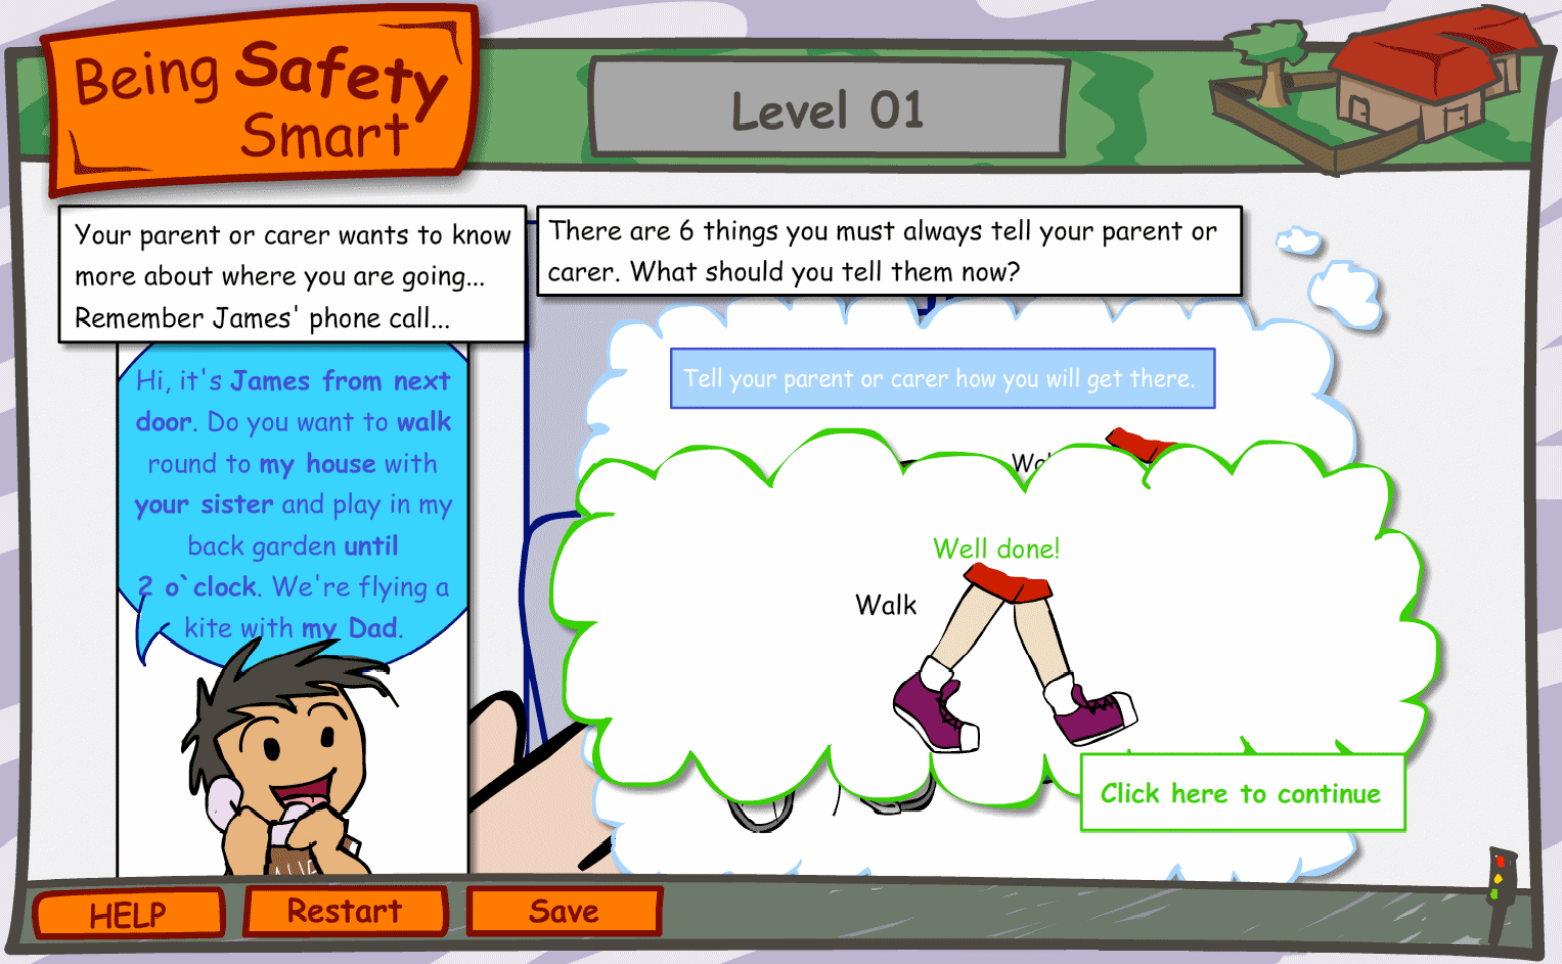
\includegraphics[width=\linewidth]{./Figuras/BSS/acerto.png}}      
\end{minipage}%
~ 
\begin{minipage}[t]{0.5\textwidth}
    \caption{\label{fig:erro}Erro no jogo}
    \vspace{0.1cm}
    \centering
    \frame{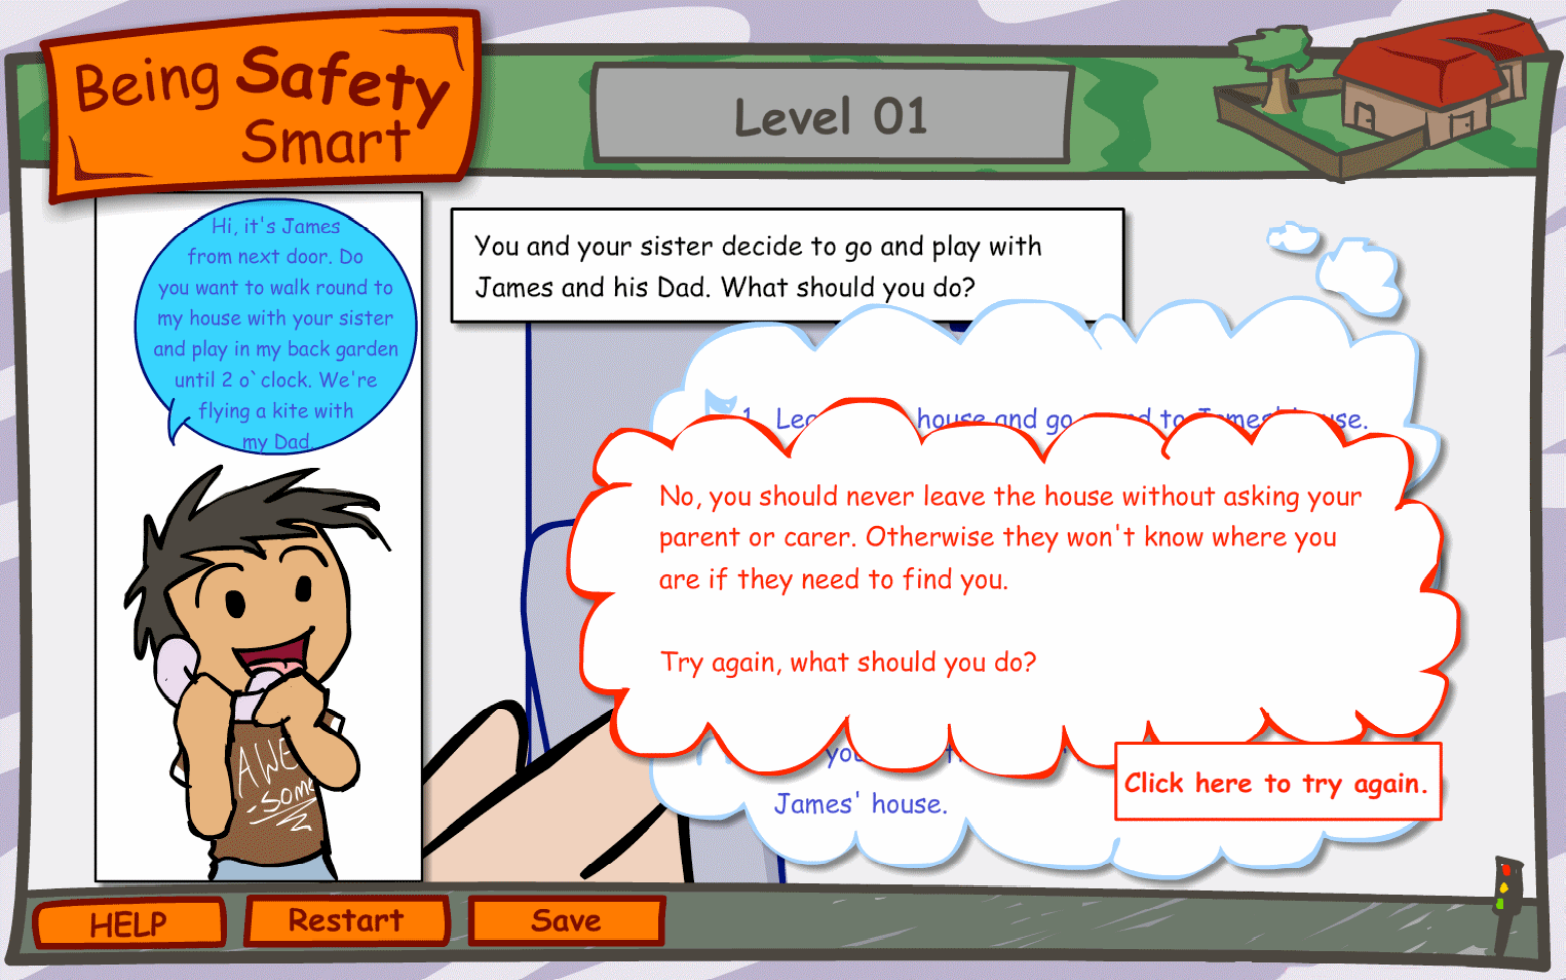
\includegraphics[width=0.99\linewidth]{./Figuras/BSS/erro.png}}
\end{minipage}

	\end{center}
  \legend{Fonte: \cite{jones2008online}}

\end{figure}



%What is Being Safety Smart?

%-Free to play online game
%-Can play at school or at home
%-Learn how to keep yourself safe
%-Play 10 mini games
%-Solve Puzzles and situations
%-Create your own character
%-Recieve certificates that you can print

A \autoref{fig:acerto} apresenta a resposta dado ao jogador quando responde corretamente uma questão. A \autoref{fig:erro} apresenta a resposta dado ao jogador quando responde erroneamente uma questão. A mensagens são apresentadas sobre a questão. Caso o jogador comenta um erro, o jogador deve voltar a questão e responde-la corretamente. Caso cometa um acerto o jogador da continuidade ao jogo. 
\end{comment}

O jogo \textit{Being Safety Smart} foi validado por meio de um processo avaliativo constituído por um grupo controle e por um grupo experimental \cite{jones2010being}. O grupo controle representa o conjunto de participantes (crianças) que não tiveram acesso ao jogo. O grupo experimental, por sua vez, representa o conjunto de participantes (crianças) que jogaram o jogo \textit{Being Safety Smart}. Ambos os grupos foram submetidos a um questionário de 35 questões de múltipla escolha. A submissão do questionário ocorreu em dois momentos distintos da pesquisa. 

%\cite{jones2010being} avaliaram Begin Safety Smart em escolas com professores, pais e filhos. O feedback sobre o Being Safety Smart tem sido muito positivo, com as crianças gostando de trabalhar no programa e querendo jogar novamente e novamente. Nossas avaliações mostraram que as crianças do programa estão muito mais conscientes de sua segurança pessoal e sabem como agir para se manterem seguras.As crianças que jogam melhoram significativamente seus conhecimentos sobre as habilidades e estratégias anti-abdução de <60 \% a> 90 \% em comparação com as crianças não participantes da mesma escola que alcançam apenas <60 \% de respostas corretas às questões de conhecimento. Além disso, as crianças que jogam apresentam maior confiança.Muito obrigado ao diretor, professores, pais e filhos de todas as escolas que participaram dos testes.

Inicialmente ambos os grupos foram convidados a responder o questionário. Neste primeiro momento o grupo experimental ainda não havia tido contado com o jogo \textit{Being Safety Smart}. A ideia desta etapa (conhecida como pré-teste) é averiguar o alinhamento no nível de conhecimento de ambos os grupos. Nesta etapa 34 crianças responderam ao questionário no grupo controle e 36 crianças responderam ao questionário no grupo experimental. Como resultado desta pré-avaliação, o grupo controle alcançou uma taxa de acerto de 67,83\% ($\sigma$ = 7,91\%), enquanto o grupo experimental obteve uma taxa de acerto no questionário de 66,11\% ($\sigma$ = 15,41\%). Os resultados demonstram que ambos os grupos compartilham o mesmo nível de conhecimento na etapa de pré-testes. Após estes resultados, o grupo experimental foi convidado a jogar o jogo. Depois de jogar e finalizar todos os níveis do jogo, ambos os grupos foram convidados a responderem novamente o mesmo questionário na etapa de pós-teste. 

O questionário foi submetido a ambos os grupos na etapa de pós-teste. A ideia desta etapa é constatar diferenças dos rendimentos dos grupos ao responderem o questionário. Nessa etapa o grupo controle consistia de 37 crianças, enquanto o grupo experimental consistia de 39. Como resultado, após responderem o questionário o grupo controle obteve uma taxa de sucesso de 69,11\% ($\sigma$ = 10,49\%), enquanto o grupo experimental obteve uma taxa de acerto de 89,97\% ($\sigma$ = 11,18\%). Os dados mostram uma nítida evolução no desempenho do grupo experimental em relação ao grupo controle, implicando assim, uma possível influência do jogo ministrado. Os resultados mostram que muito mais crianças aprendem a se protegerem devidamente depois de concluir o jogo. %O mesmo aumento significativo na compreensão das estratégias de segurança não é observável com o grupo de controle.




%[QUantidade grupo controle = 37]34(antes)
%[Quantidade grupo testado = 39]36(antes)

%O Children’s Knowledge Questionnaire  consiste em 35 perguntas de duas escolhas (verdadeiro/falso (o não sei)). Esse questionario foi submetido antes e após os experimentos (apenas as crianças do grupo testado). Antes do início do experimento, não havia diferença significativa no conhecimento de segurança das crianças entre os grupos de controle e experimental (a média de respostas corretas de ambos os grupos foi 28 questões corretas) [sendo 23.74 para o grupo controle com desvio padrão de 2.767 e 23.14 para o grupo testado com desvio padrão de 5.394]. Após os testes o grupo controle se manteve dentro do desvio padrão com 24.19 pontos e 3.673 de desvio padrão. Já o grupo testado teve a nota de 31.49 com desvio de 3,913. Esses dados compararam o conhecimento de segurança pessoal de cada criança antes e depois do programa. Os resultados indicaram que o conhecimento das crianças sobre segurança pessoal melhorou significativamente, após o envolvimento no programa.  



%Sendo Safety Smart foi avaliado em escolas usando grupos de controle de contrapartida. A avaliação teve como objetivo avaliar a eficácia do projeto em fornecer conhecimentos e habilidades de conscientização sobre segurança para crianças e a retenção de conhecimentos e habilidades. Em cada escola as crianças foram divididas em dois grupos: experimental (participaram com o ambiente do jogo multimídia de conscientização de segurança) e controle (sem acesso aos materiais de conscientização sobre segurança). Depois que a avaliação foi concluída, o grupo de controle também completou o jogo, minimizando assim qualquer chance de estarem menos preparados para abduções potenciais. Os pais foram solicitados a consentir que seus filhos participassem de qualquer um dos grupos experimentais e de controle, e os professores foram instruídos a minimizar quaisquer possibilidades de habilidades e estratégias de conscientização sobre segurança infantil a serem discutidas entre as crianças nos grupos experimental e controle \cite{jones2010being}.

%A avaliação foi feita com adpatações dos questionarios: Skills Questionnaire e Children’s Safety Knowledge (outros questinarios contemplaram o processo avaliativo para pais e professores). Para medir a pré e pós-compreensão da criança de situações de abdução e o Inventário de Autoestima Livre de Cultura de Batalha para medir a autoestima e a confiança da criança \cite{jones2010being}. 

O jogo foi ministrado ao grupo experimental durante o período de dois meses. %A cada semana as crianças eram convidadas a completar um nível do jogo. 
Durante este processo os profissionais e pesquisadores envolvidos foram devidamente treinados a conduzir os experimentos. Além disso, os pais das crianças tiveram participação ativa neste processo, sendo responsáveis por notificarem qualquer alteração no comportamento das crianças como ansiedade ou angústia. O jogo então manifesta dois resultados positivos, o primeiro de ampliar os conhecimentos das crianças acerca sua segurança pessoal e o segundo pelo fato do jogo não manifestar qualquer desconforto ou mudança inadequada de comportamento aos jogadores. 


%Os experimentos duraram oito semanas. As crianças completaram um nível por semana durante 8 semanas sob a orientação e apoio do professor. Durante o processo, a equipe de pesquisa (os profissionais envolvidos receberam treinamento adquado. Além disso, foram implementados procedimentos para apoiar quaisquer casos de abuso sexual infantil revelados ao pesquisador), professores e pais monitoraram o comportamento da criança quanto ao uso inadequado de estratégias aprendidas, ansiedade, angústia e confusão, e apoiam a criança com cuidado e ensino adicionais.

%Os resultados mostram que muito mais crianças entendem as estratégias de segurança corretas depois de concluir o programa, em comparação com antes de usá-lo. O mesmo aumento significativo na compreensão das estratégias de segurança não é observável com o grupo de controle. %Além disso, para alguns dos itens listados abaixo, pode ser visto para o grupo de controle que a porcentagem de respostas incorretas é maior do que a porcentagem de respostas corretas.


%[acho que um teste foi realizado com outro grupo para constatar se o conhecimento das crianças mudou com o andamento do programa = Este resultado indica que o conhecimento de segurança pessoal das crianças não mudou ao longo do tempo do programa]



%COmo resultado dessa pesquisa (feedback) descobriu-se que o "jogo do labirinto" era muito difícil de controlar e as penalidades por seguir uma rota insegura eram frustrantes para o grupo de crianças em idade alvo. O jogo foi redesenhado e testado para fornecer penalidades imediatas e limitadas no tempo e para fornecer jogabilidade simples com as teclas de controle de seta do teclado.


%Being Safety Smart: Social Issue Game for Child Protective Behaviour Training (grupo controle)


%https://web.archive.org/web/20160229090036/http://www.beingsafetysmart.com.au/BSS/

%https://www.scienceopen.com/document_file/4c902f75-be26-4dd5-929f-59288a948b01/ScienceOpen/151_Jones.pdf

\section{Orbit Rescue}\label{sssec:Orbit}

%O jogo Orbit, planos de aula e informações do site foram desenvolvidos em colaboração com assistentes sociais, conselheiros, psicólogos, pesquisadores em educação, professores, pais e alunos. O programa está alinhado com o currículo de Queensland e planos de aula abrangentes são fornecidos para ajudar os professores a usar os recursos de forma eficaz. Os professores podem acessar uma seção dedicada do site do Orbit que contém recursos adicionais, atividades em sala de aula, informações sobre CSA e prevenção e materiais de treinamento para ajudar os professores a usar o Orbit. Os professores podem adotar os recursos ou usá-los sem modificação e também são incentivados a estender as aulas e usar o site para compartilhar esses novos recursos com outras pessoas. A Orbit também recomenda e descreve maneiras que os professores podem trabalhar com o apoio relevante existente nas escolas, como orientadores de alunos e funcionários de bem-estar para entregar o programa de prevenção de CSA. O site Orbit fornece procedimentos práticos para ajudar os funcionários da escola a responder adequadamente a uma divulgação do CSA, incluindo requisitos de relatórios obrigatórios e maneiras de garantir que o bem-estar da criança seja salvaguardado.

\textit{Orbit Rescue}\footnote{\textit{Orbit Rescue} é um jogo sério desenlvido pela Universidade de Sunshine Coast e lançado em 2012. Mais informações sobre o jogo podem ser acessadas em seu portal: \url{http://orbit.org.au/}.} é um jogo no estilo aventura projetado para conscientizar as crianças sobre o abuso sexual infantil. O jogo é voltado a atender crianças entre oito e dez anos de idade. Dentre os ensinamentos ministrados pelo jogo estão conceitos de: privacidade corporal, comunicação, confiança e defesa pessoal. Os quatro ensinamentos se traduzem em quatro fases a serem acessadas no jogo, que possui texto e dublagem em inglês, apenas. A \autoref{fig:selecao} ilustra a tela de seleção de fases do jogo.

%O objetivo do Orbit é ajudar as crianças a desenvolver relacionamentos, confiança, bem-estar, valor próprio, estima e segurança, e construir redes de apoio, conhecimento comunitário e responsabilidade. O Orbit dá a crianças e adultos a oportunidade de serem apoiados, de discutir o abuso sexual infantil e de quebrar o silêncio que serve para proteger os perpetradores.

\vspace{-0.2cm}

\begin{figure}[htb]

	\caption{\label{fig:selecao}Tela de seleção das fases do jogo \textit{Orbit Rescue}.}
  \begin{center}\vspace{-0.3cm}
    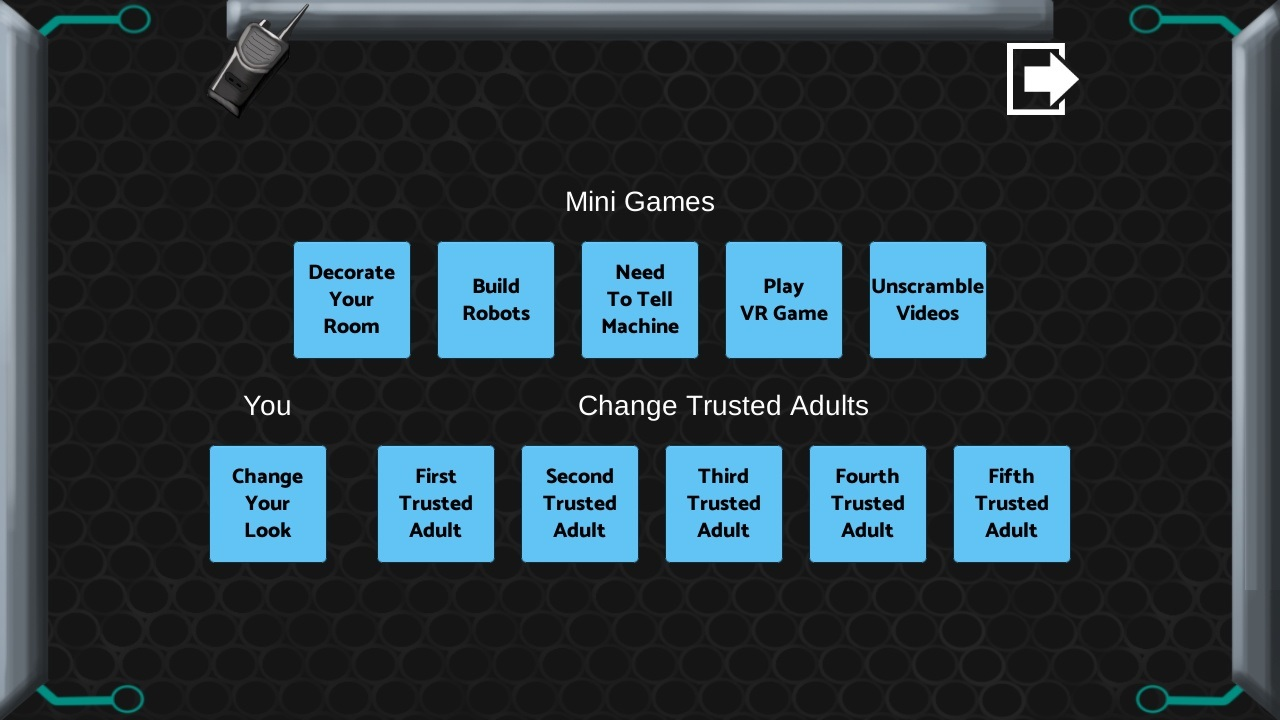
\includegraphics[width=0.94\linewidth]{./Figuras/Orbit/OrbitFases.jpg}
	\end{center}\vspace{-0.5cm}
  \legend{Fonte: \citeonline{steiler2012orbit}}

\end{figure}

\vspace{-0.3cm}

O jogo \textit{Orbit Rescue} dispõem de dois canais de acesso as fases do jogo. 
As fases do jogo podem ser acessadas em determinados cenários, ou podem ser acessadas por meio de um ícone que leva a uma tela de seleção de fases como mostra a \autoref{fig:selecao}. Cada fase se traduz em um minijogo com dinâmica e ensinamentos distintos entre si, cada fase contém uma quantidade variadas de níveis a serem explorados. Há ainda conceitos não ministrados nos minijogos, com a questão dos adultos de confiança. Tal conceito é passado com o intuito de ensinar ao jogador a reconhecer e identificar pessoas em quem possa confiar. O jogador deve então, personificar no jogo cinco adultos de confiança. Indiretamente o jogador aprende a sempre estar acompanhado por alguém de confiança, pois o personagem fabricado acompanha o personagem do jogador em grande parte da história do jogo. Por fim, a \autoref{fig:selecao} também apresenta algumas opções que não estão associados a um contexto pedagógico direto, como a customização do personagem ou do quarto do personagem. Por não terem significância didática, tais opções não são apresentadas nesse trabalho. 

\begin{wrapfigure}[22]{r}{3.5cm}%pulando 22 linhas
  \vspace{-5pt}
  \caption{\label{fig:orbitniveis}Níveis.\vspace{5pt}}

  \subfloat[Nível 1\label{fig:11}\vspace{-5pt}]{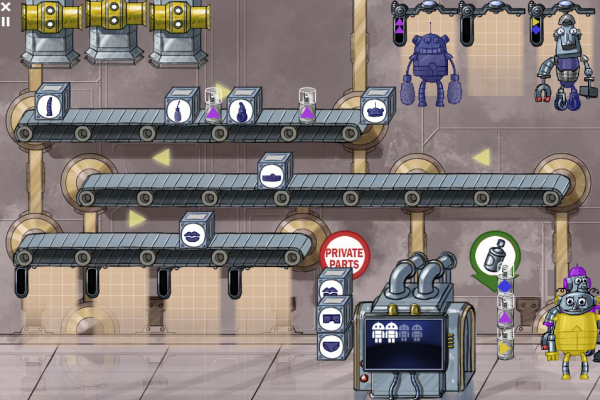
\includegraphics[width=\linewidth]{./Figuras/Orbit/robot-factory-screenshot.png}}\vspace{-3pt}
  \\
  \subfloat[Nível 2\label{fig:22}\vspace{-5pt}]{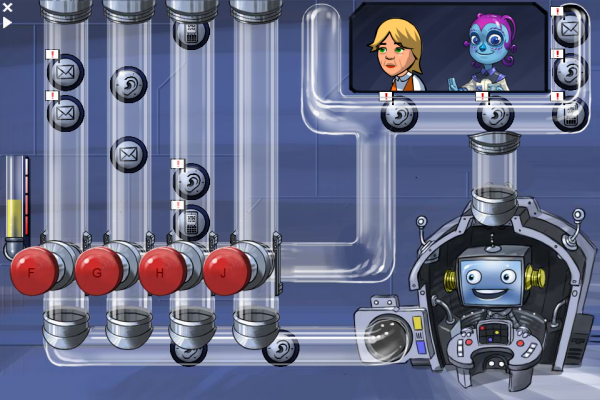
\includegraphics[width=\linewidth]{./Figuras/Orbit/need-to-tell.png}}\vspace{-3pt}
  \\
  \subfloat[Nível 3\label{fig:33}\vspace{-5pt}]{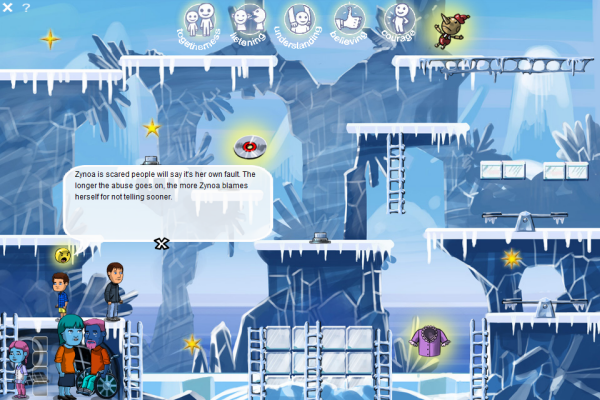
\includegraphics[width=\linewidth]{./Figuras/Orbit/speak-up.png}}\vspace{-3pt}
  \\
  \subfloat[Nível 4\label{fig:44}\vspace{-5pt}]{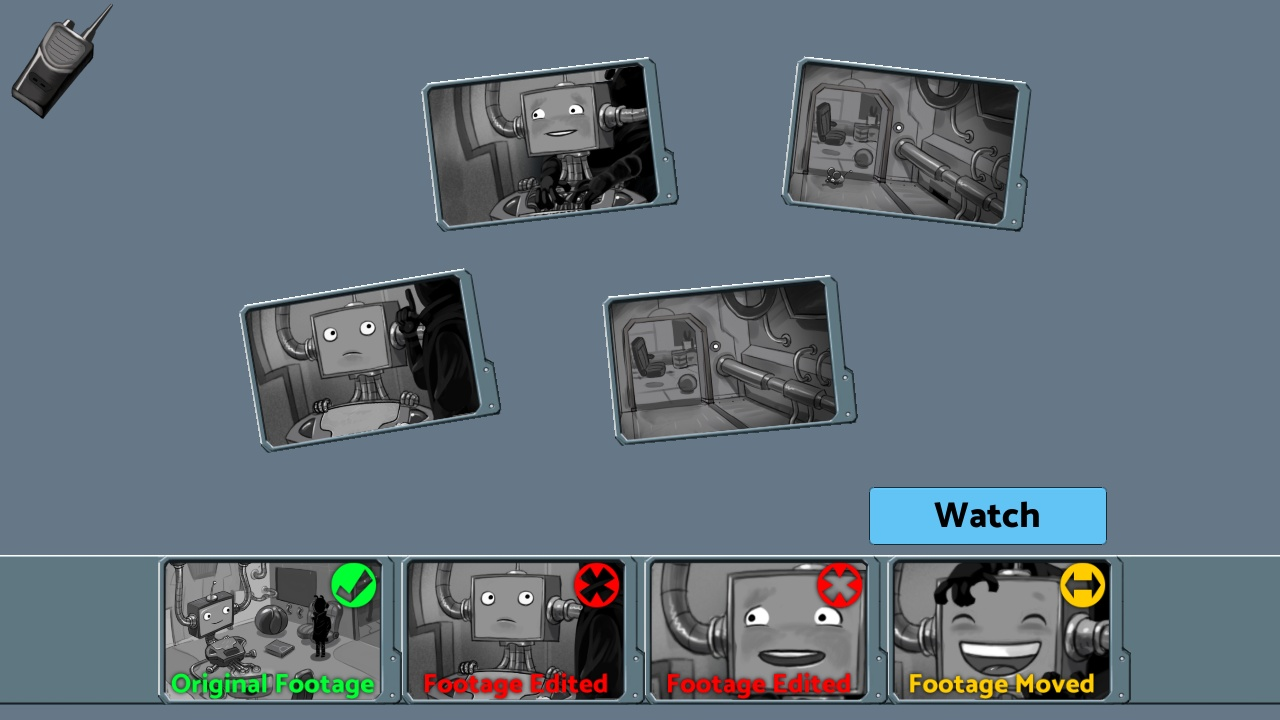
\includegraphics[width=\linewidth]{./Figuras/Orbit/cameras.jpg}}\vspace{-3pt}
  \vspace{-8pt}
  \legend{Fonte: \citeonline{steiler2012orbit}}%eu paguei outros nao citados aqui, como fazer a referencia?
  %india (mas não governamental)
\end{wrapfigure}

A \autoref{fig:orbitniveis} apresenta os quatro minijogos ministrados pelo jogo \textit{Orbit Rescue}. Cabe salientar que o jogo segue uma narrativa, por tal razão as fases não se encontram disponíveis ao jogador em um momento inicial. A ordem estabelecida na \autoref{fig:orbitniveis} representa a ordem que as fases vão sendo liberadas ao jogador. Inicialmente o jogador é ensinado sobre sua privacidade corporal (Figura \ref{fig:11}), nesta fase o jogador aprende quais são as partes íntimas e que elas não devem ser tocadas. Em seguida o jogador é ensinado a se comunicar devidamente (Figura \ref{fig:22}), o intuito desta fase é ajudar a criança a identificar situações que precisam ser reportadas para adultos de confiança. Conforme a história do jogo avança a criança aprende em um dado momento a ganhar confiança (Figura \ref{fig:33}), essa fase se objetiva a ensinar a superar episódios de abuso e como proceder em tais situações. Por fim, na sua última fase o jogo discorre sobre as abordagens utilizadas pelos agressores sexuais  (Figura \ref{fig:44}), o jogador então deve identificar neste momento como é a atuação de um agressor sexual e aprender a reconhecer tais estratégias desde seu momento inicial e a tomar as devidas medidas. Embora os mini-jogos acompanhem a história e o enredo do jogo, o jogador é livre para acessar qualquer uma das fases liberadas sempre que desejar, sem quaisquer prejuízos a história do jogo. 

%Todos os mini-jogos estão relacionados com o enredo estabelecido pelo jogo. As fases são liberadas ao jogador conforme a história do jogo avança.

%Por exemplo, o minijogo Robot Factory exigia que as crianças construíssem robôs para a nave "tocando" e movendo partes dos robôs para construção, enquanto "não tocavam" outras partes (boca, tórax e área coberta pela cueca). No minijogo Need to Tell Machine, a criança deve identificar quais cenários devem ser contados aos seus adultos de confiança e quais não precisam ser contados, e no minijogo Speak Up a criança brinca ao lado de um de seus adulto de confiança para ajudar uma 'criança no jogo' a superar seu medo de revelar o abuso ao adulto de confiança.


%O jogo se passa em uma espaçonave composta por alienigenas e robos, conforme pode ser obvservado.


\vspace{-0.1cm}

O jogo \textit{Orbit Rescue} passou por um processo de validação com o intuito de averiguar aumento no conhecimento dos alunos sobre os conceitos de abuso infantil e sua capacidade de reconhecer e responder a situações hipotéticas de abuso. Três grupos de crianças entre oito e dez anos foram selecionadas (média de 45 crianças por grupo). O primeiro grupo foi submetido ao jogo \textit{Orbit Rescue} e a um plano de ensino de apoio. O segundo grupo foi submetido apenas ao jogo. E o terceiro grupo não foi submetido nem ao jogo nem ao plano de ensino \cite{jones2020serious}.

\vspace{-0.1cm}

O processo de validação durou cerca de quatro meses. Na primeira etapa (pré-teste) os grupos foram submetidos a um questionário de 31 questões. O desempenho dos três grupos beirou uma taxa de acerto de 75\% no questionário. Na etapa final (pós-teste), o grupo controle manteve o mesmo resultado no questionário. Entretanto os outros dois grupos tiveram uma taxa de 90\% de acerto no questionário. Olhando individualmente, as crianças que mais obtiveram sucesso no questionário foram as que finalizaram o jogo, sendo constatado uma maior número de crianças que finalizaram o jogo no grupo que recebeu o plano de apoio. A pesquisa manifestou então dois resultados positivos, o primeiro provando a eficácia do jogo e o segundo evidenciando a importância de um plano de apoio para ampliar as taxas de conclusão do jogo. 

 

%O processo de validação do jogo é constutido por um pré-teste e por um pós-teste no qual um questionário de 31/17 questões de multipla escolha foi submetido aos grupos (dois questionarios).


%. Os alunos que não concluíram o jogo não melhoraram significativamente seu conhecimento sobre a prevenção da CSA, conforme medido pelo CKAQ e CKAQ SF, enquanto os alunos que concluíram o jogo mostraram aumentos estatisticamente significativos.

%nossos resultados indicam que os alunos devem se envolver com o jogo e continuar o suficiente para receber os ganhos de conhecimento

%O jogo foi projetado para ser jogado ao longo de um período de 5 a 10 semanas, construindo gradualmente o conhecimento das crianças enquanto elas brincam (podem ser minitrado em sala de aula ou em casa)

%Em ambas as análises do CKAQ (31 itens e 17 itens), não houve diferenças estatisticamente significativas entre as pontuações para o grupo de jogo apenas e grupo de jogo e aula.

%as crianças que jogam o jogo até o final têm probabilidade de obter ganhos de conhecimento, independentemente de as atividades extras em sala de aula serem realizadas em torno do jogo. No entanto, dada a natureza do conteúdo, recomendamos que o jogo seja jogado com o conhecimento de um dos pais ou professor. (a maior diferença entre o grupo de jogou o jogo e o grupo que jogou e teve aulas é que menos crianças finalizaram o jogo no grupo que apenas jogou. Desconsiderando essas crianças o desempenho das crianas em ambos os grupo foi particamente o mesmo)

%Os experimentos duraram cerca de 4 meses. Eles se usaram esse questionario \cite{tutty2003children}, mas removeram duas questões (33-2=31) devido a terem criticas. Fizeram um questionario resumido, para contemplar o jogo como um todo, pois o jogo nao ministrava todos os conceitos necessarios para compreender e responder de forma correta todo o questionario, entao fizeram um resumido de 17 perguntas (porem ela deve baixa confiabilidade/entao nao gostaram muito [incerta demais]).  Já o 'original' usado no estudo teve confiabilidade boa e medida adequada .

%os aprendizados proporcionados foram medidos pré e pós-intervenção usando o Children's Knowledge of Abuse Questionnaire-Revised (CKAQ-R-III), e uma forma abreviada (SF) do CKAQ mapeado para os objetivos de aprendizagem do jogo.

%As crianças nos grupos de jogo de Orbit e jogo de Orbit e de lição aumentaram significativamente (p <0,001) suas pontuações no pós-teste com o CKAQ SF, enquanto as do grupo de controle não. Além disso, as crianças que completaram todos os jogo de forma significativa (p <0,001) aumentaram suas pontuações no CKAQ pós-teste, enquanto aquelas que não completaram o jogo não.

%O desemenho do grupo controle e dos demais antes do jogo (e do controle após) foi de 75\% já o desemepnho ficou entrono de 93\% para o grupo de jogou o jogo e jogou o jogo e teve aula \cite{jones2020serious}. 


%https://sci-hub.scihubtw.tw/10.1080/13603116.2013.860195

%https://ro.ecu.edu.au/cgi/viewcontent.cgi?article=2270&context=ajte [antes de avaliar o jogo] = Boys and CSA Pr ys and CSA Prevention: Issues Surr ention: Issues Surrounding Gender and ounding Gender and Approaches for Prevention

%https://sci-hub.do/10.1016/j.chiabu.2020.104569









%O Engage Research Cluster lançou um jogo interativo chamado ‘Orbit’, que foi projetado para ajudar a combater o abuso sexual infantil. O Orbit oferece uma variedade de atividades que ajudam a desenvolver confiança, bem-estar e habilidades de resolução de problemas em crianças, e faz parte de um pacote que inclui planos de aula e materiais de apoio para professores.


%O Orbit se concentra no desenvolvimento progressivo de conhecimentos e habilidades essenciais. Em vez de depender do aprendizado mecânico baseado em regras, o jogo incentiva o desenvolvimento de relacionamentos, confiança, bem-estar, valor próprio, estima e segurança. O programa também trabalha com adultos para construir redes de apoio, conhecimento da comunidade e responsabilidade. Além disso, o Orbit oferece aos adultos de confiança a oportunidade de receber apoio e discutir o abuso sexual infantil e quebrar o silêncio que serve para proteger os perpetradores. O jogo em si se baseia em três conceitos: 





%\begin{itemize}
%  \item desenvolver uma compreensão apropriada para a idade do que é abuso %sexual
%  \item reconhecer que o abuso sexual é ilegal e que não é culpa da criança
%  \item entender que se ele / ela está sendo abusado sexualmente, ele precisa %contar a todos os adultos de sua rede de apoio.
%\end{itemize}

%Esses conceitos são abordados através de mini-jogos conditos no jogo. No minijogo Robot Factory, o jogador deve montar uma série de robôs arrastando as partes do corpo do robô apropriadas para a planta. Ela coloca as partes públicas do corpo (cabeça, braços, pernas e estômago) na planta, mas deixa as partes privadas (boca, tórax e área coberta pela cueca) rolar para fora da esteira rolante para a seção de partes privadas. Uma vez que as partes públicas do robô foram montadas, o jogador coloca o robô parcialmente montado na fila de montagem. O robô vai para o camarim, onde fixa suas partes íntimas e é pintado.


%No minijogo Need to Tell Machine, o jogador ajuda a retreinar o Need to Tell Machine, marcando algumas histórias de treinamento como coisas que uma criança precisaria contar a um adulto de confiança e outras como coisas que uma criança não precisaria. dizer (mas poderia se quisesse). Em seguida, ela ajuda a Need to Tell Machine a enviar os itens marcados com "necessidade de contar" para um dos adultos de confiança de Sammy.


%Speak Up é um jogo que aborda as muitas barreiras emocionais e psicológicas que podem impedir as crianças de revelar o abuso a seus adultos de confiança. É um jogo de plataforma baseado em quebra-cabeças, projetado para jogar lado a lado (duas pessoas em um teclado de computador) para que o jogador possa jogar com um de seus adultos de confiança. Na sala de aula, duas crianças podem jogar o jogo juntas.


%ATE AQUI TODA A INFORMACAO VEIO DO SITE DO JOGO

%https://sci-hub.do/10.1016/j.chiabu.2020.104569 



%https://eprints.qut.edu.au/109072/1/OrbitTeachersGuide.pdf


\section{Cool and Safe}\label{sssec:CeS}

\textit{Cool and Safe}\footnote{\textit{Cool and Safe} é um jogo desenvolvido pela Universidade de Frankfurt lançado ao público em 2013. Mais informações sobre o jogo podem ser acessadas em seu portal: \url{https://www.coolandsafe.eu/}.} é um jogo para navegadores voltado para prevenção da violência sexual de crianças. O jogo é destinado a atender crianças na faixa dos sete aos doze anos. O jogo almeja prevenir as crianças do abuso sexual infantil, fortalecendo as habilidades de autoafirmação, transmitindo estratégias para lidar com situações perigosas e expandindo o repertório comportamental das crianças \cite{pajalakasvatustieteiden}. O jogo atende crianças de tênue idade, por tal razão todos os conceitos são apresentados de forma escrita e verbal em alemão e em francês (a depender da configuração do idioma). A página inicial do portal do jogo é mostrada na \autoref{fig:portal}.

%http://jultika.oulu.fi/files/nbnfioulu-201808232667.pdf
%\cite{pajalakasvatustieteiden}


\begin{figure}[htb]

	\caption{\label{fig:portal}Portal do jogo \textit{Cool and Safe}.}
  \begin{center}%\vspace{-0.3cm}
    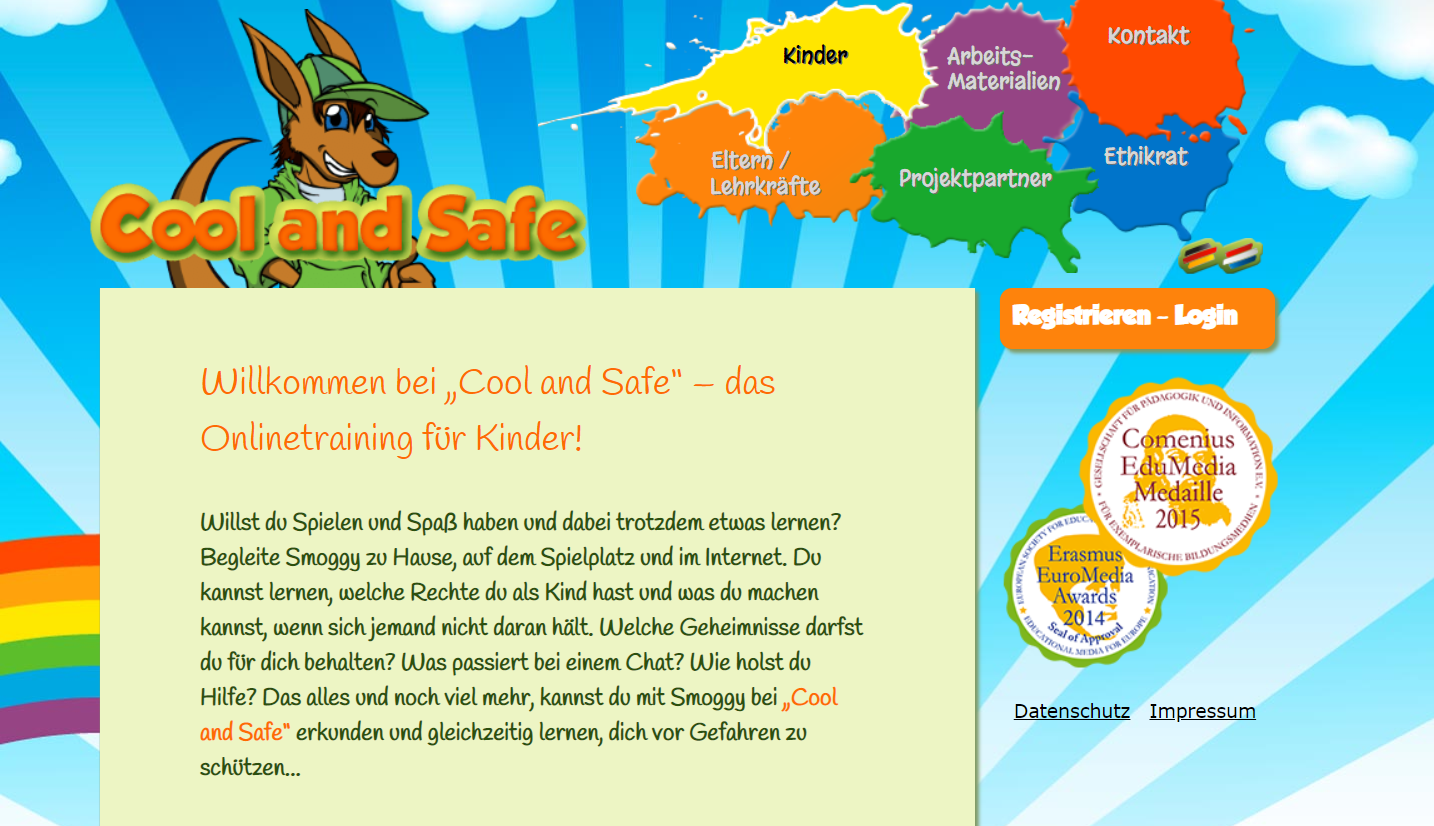
\includegraphics[width=\linewidth]{./Figuras/Cool/coolSafe.png}
	\end{center}%\vspace{-0.5cm}
  \legend{Fonte: \citeonline{fingerleabschlussbericht}}

\end{figure}

A \autoref{fig:portal} apresenta a tela principal do portal do jogo \textit{Cool and Safe}. Nesta tela é possível observar as opções para troca de idioma, simbolizadas pelas bandeiras da França e da Alemanha. O jogo requer um cadastro para acesso, sendo necessário cadastrar um nome, senha, dia e mês de aniversário. Após o cadastro, o jogador obtém livre acesso ao jogo. Ao começar a jogar, o jogador é apresentado a vários clipes de filmes, histórias e tarefas nos quais deve ponderar e escolher entre diferentes alternativas \cite{mueller2012web}. 

\begin{wrapfigure}[24]{r}{3.8cm}%pulando 22 linhas
  \vspace{-5pt}
  \caption{\label{fig:coolniveis}Níveis.\vspace{5pt}}

  \subfloat[Nível 1\label{fig:111}\vspace{-5pt}]{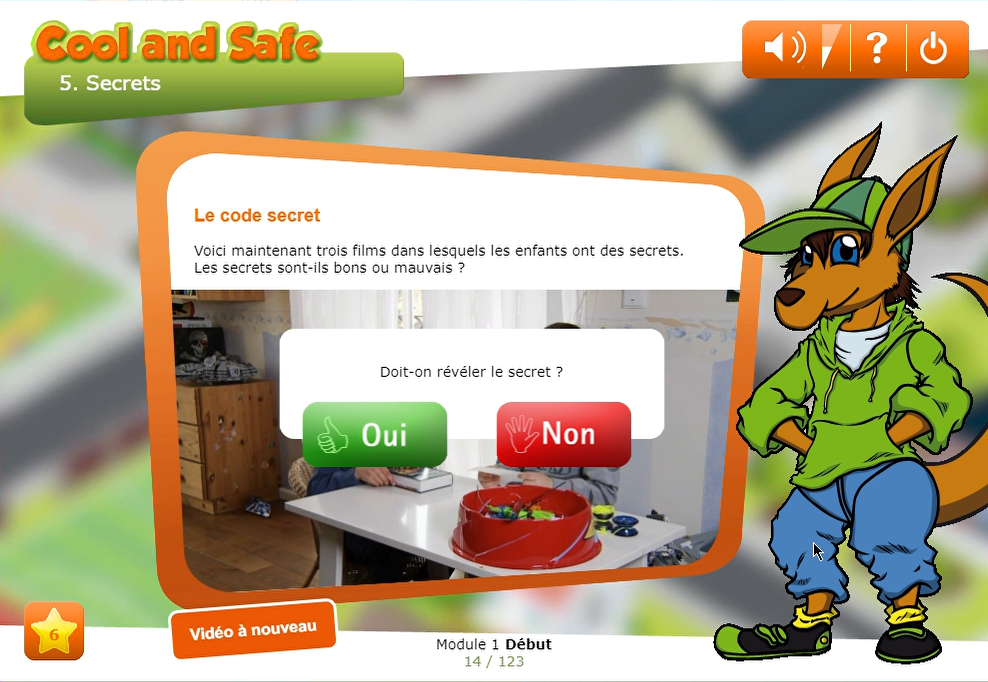
\includegraphics[width=\linewidth]{./Figuras/Cool/nivel11.png}}\vspace{-3pt}
  \\
  \subfloat[Nível 2\label{fig:222}\vspace{-5pt}]{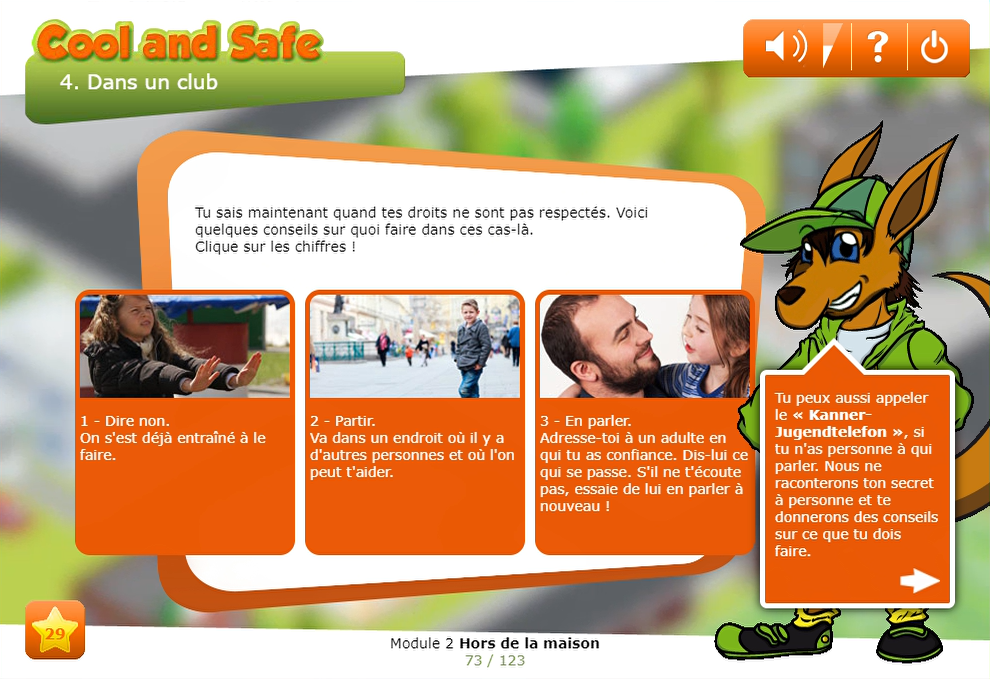
\includegraphics[width=\linewidth]{./Figuras/Cool/nivel222.png}}\vspace{-3pt}
  \\
  \subfloat[Nível 3\label{fig:333}\vspace{-5pt}]{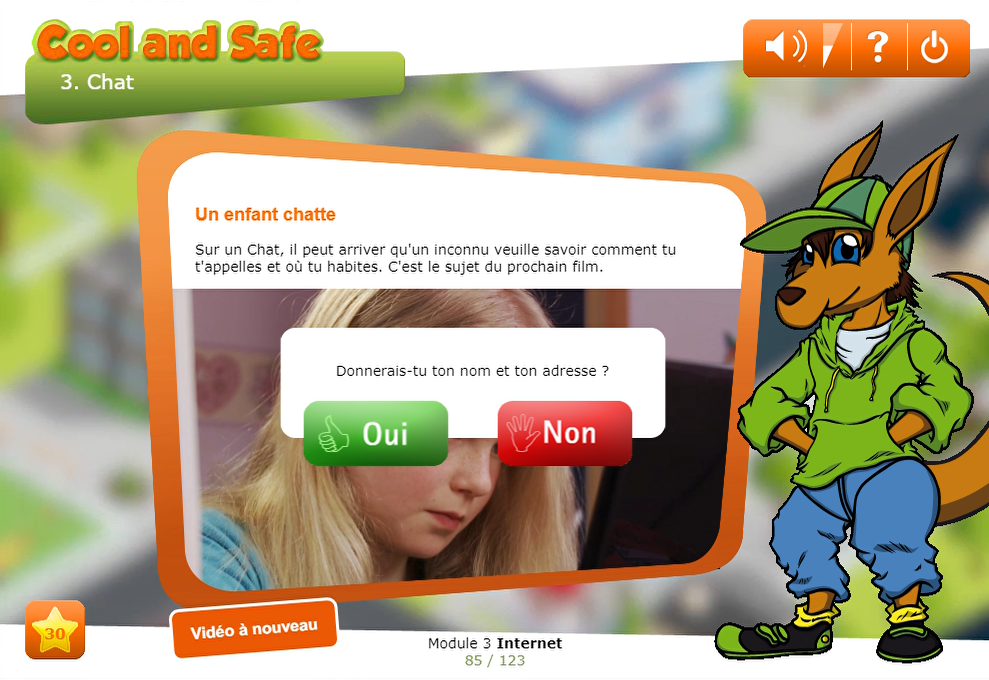
\includegraphics[width=\linewidth]{./Figuras/Cool/nivel3.png}}\vspace{-3pt}
  \\
  \subfloat[Nível 4\label{fig:444}\vspace{-5pt}]{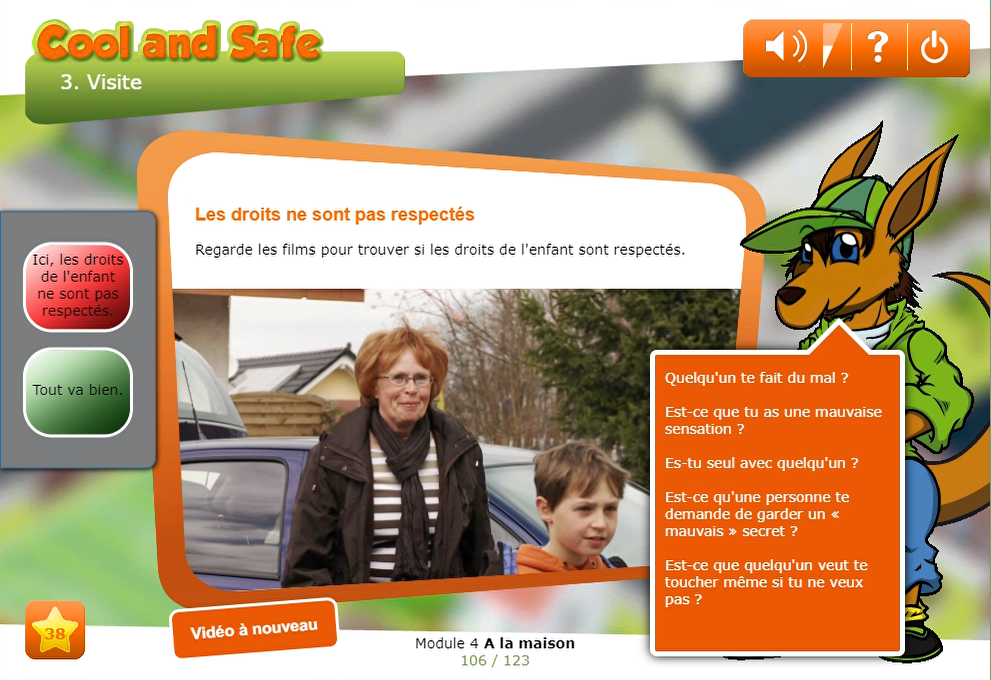
\includegraphics[width=\linewidth]{./Figuras/Cool/nivel4.png}}\vspace{-3pt}
  \vspace{-8pt}
  \legend{Fonte: \citeonline{fingerleabschlussbericht}}%eu paguei outros nao citados aqui, como fazer a referencia?
  %india (mas não governamental)
\end{wrapfigure}


O jogo é constituído por cinco módulos de ensinamentos para as crianças. Cada módulo corresponde a um conceito distinto a ser apreendido pelo jogador. A sequência dos módulos é fixa e não pode ser alterada pelo usuário. Portanto, não é possível realizar módulos individuais separadamente, além disso o jogador não possui flexibilidade para retornar para um determinado módulo após concluí-lo. O primeiro módulo (Figura \ref{fig:111}) consiste em apresentar alguns conceitos básicos aos jogadores como interpretar sentimentos, guardar ou não segredos e conversar com os pais. O segundo módulo (Figura \ref{fig:222}) consiste em um tópico mais avançado voltado a educar sobre situações que podem ocorrer fora de casa como aceitar doces de estranhos, identificar situações perigosas e recusar caronas de estranhos. O terceiro módulo (Figura \ref{fig:333}) é destinado a ensinar os menores a usar adequadamente a \textit{internet}, neste módulo o jogador é ensinado a usar adequadamente as redes sociais, não adicionar estranhos e não dar informações pessoais a estranhos. O quarto módulo (Figura \ref{fig:444}) busca educar as crianças sobre situações que podem acontecer dentro de casa, aqui a criança é ensinada sobre seus direitos e deveres, ensinada a não abrir a porta para estranhos e ensinada a denunciar a quebra de seus direitos para outras pessoas. O último módulo (sem figura representativa) apresentam uma compilação de algumas lições aprendidas nos módulos anteriores sendo uma revisão.%servindo como uma espécie de revisão. 

\begin{comment}
O conceito “Cool and Safe”  foi criado com o objetivo de ensinar as crianças a agir e capacitá-las para o exercício de seus direitos. De acordo com a jurisprudência do Tribunal Constitucional Federal, o artigo 6º da Lei Básica representa indiretamente um reconhecimento da própria dignidade humana da criança e o direito ao desenvolvimento pessoal (Hurrelmann \& Andresen, 2007). Os temas tratados em “Cool and Safe” dizem respeito a vários direitos da criança, que também estão previstos na Convenção das Nações Unidas sobre os Direitos da Criança. Por exemplo, nos termos do Artigo 34, a proteção contra o abuso sexual é formulada como um mandato dos estados da ONU. A proteção contra o uso da força (Artigo 19) também está ancorada ali. O mesmo se aplica à proteção da vida privada e da honra das crianças (artigo 16), bem como à proteção das crianças e dos jovens no que diz respeito ao acesso aos meios de comunicação (artigo 17). A crescente disseminação da Internet cria novos riscos na forma de contatos por motivação sexual ou bullying na Internet - mas também novas oportunidades. Sete assuntos são abordados no jogo:

\begin{itemize}
  \item Se distanciar de situações perigosas = fique longe pelo menos 3 passos, se um estranho ou um atomobilista falar com você
  \item Dizer NÃO
  \item Evitar situações perigosas =Afaste-se quando uma situação for desagradável ou puder se tornar perigosa.
  \item Procurar ajuda
  \item Conversar com o pais (ou pessoas confiaveis)
  \item Ligar para uma linha de denúncia (Kanner Jugendtelefon)
  \item Chamar a polícia
\end{itemize}


"Cool and Safe" é um treinamento baseado na web que é realizado no computador. Portanto, é necessária uma sala de informática para a implementação na aula, na qual um PC com internet está disponível para cada criança.




Cool and Safe é um programa de prevenção baseado na web voltado para crianças em idade escolar. O principal objetivo de “Cool and Safe” é prevenir o abuso sexual infantil, ensinando conhecimentos sobre comportamentos seguros, toques apropriados e inadequados, bem como segredos bons e ruins. Como os infratores podem ser estranhos e também familiares para a criança e podem atacá-los pessoalmente ou pela Internet, a questão é abordada em relação a três configurações diferentes da vida cotidiana das crianças: 1) interações com estranhos, 2) interações no Internet e 3) interações com conhecidos ou familiares. O programa está disponível na Internet e pode ser acessado gratuitamente em www. coolandsafe.eu (os idiomas disponíveis são alemão e francês). "Cool and Safe" é dividido em cinco unidades temáticas que devem ser concluídas em uma ordem predefinida. A unidade um contém os tópicos sentimentos ruins e bons sentimentos, bem como segredos bons e ruins. Além disso, é explicado que toda criança tem o direito de decidir quem pode tocá-la. Na unidade dois, o tópico do perigo do estranho é discutido. As crianças aprendem que devem manter distância dos carros e que têm o direito de recusar falar com estranhos quando estão sozinhas. Estratégias de segurança para situações ambivalentes ou de risco são discutidas. A unidade três concentra-se em tópicos típicos do uso da Internet, como solicitações de amizade em redes sociais, respostas a assédio em programas de bate-papo e proteção de informações privadas. O tópico de abuso sexual por conhecidos e familiares é abordado na unidade 4. As crianças são ensinadas que ninguém tem o direito de machucá-las ou de tocá-las nas partes íntimas de seu corpo. Na unidade cinco, todos os conteúdos do treinamento são repetidos e resumidos. A conclusão de todo o programa leva cerca de duas horas. A conclusão do programa pode ser pausada a qualquer momento e pode ser continuada posteriormente. Com a ajuda de um apelido e senha, as crianças podem acessar o treinamento a qualquer momento. Como o treinamento é projetado para crianças do ensino fundamental, o treinamento é totalmente lido em voz alta por uma figura de tutor que orienta as crianças durante o treinamento. As crianças são envolvidas no programa por vários clipes de filmes, histórias, tarefas e jogos e podem escolher entre diferentes alternativas de comportamento.



``« Cool and Safe » est gratuit pour un usage privé. La formation a été développée en tenant compte des découvertes scientifiques et grâce à de nombreuses années d'expérience en matière de prévention de la violence des enfants et adolescents. Une première évaluation de l'université Goethe de Francfort a donné des résultats positifs.'' ``« Cool and Safe » est actuellement le seul programme en Allemagne et au Luxembourg proposant ce type de jeu dans cette ampleur en allemand et français.'' [site oficial]
\end{comment}
%https://www.coolandsafe.eu/index.php

%Essa trabalho avaliou crianças, metade jogaram o jogo 'Cool and safe' e a outra metade não jogaram. \cite{fingerleabschlussbericht} [ter cuidado com esse tipo de pesquisa, como o livro de metodologia diz na página 11]
%[para medir a retenção de conhecimento das crianças foi usado: Questionário de Conhecimento de Abuso Infantil de Tutty (1997)]
%[O treinamento não revelou efeitos colaterais indesejáveis, como desconfiança aumentada, ansiedade ou influências negativas na consciência emocional.] = EM alemão, claro.
%[não é possível tirar conclusões dos resultados do exame do questionário disponível aqui sobre se o risco real de se tornar vítima de abuso sexual é realmente menor para as crianças participantes] = ALemão
%[no caso de uma questão difícil e sensível, como abuso sexual, deve-se considerar cuidadosamente como a informação é preparada, apresentada e transmitida.] = Alemão
%[Uma vantagem de um treinamento baseado na Web como o CaS é a grande variedade com relativamente pouco gasto de recursos.] = Alemão

%NOTA: aqui esta a grade curricular alemã, verificar se o jogo é ministrado.
%https://www.bmbwf.gv.at/Themen/schule/schulpraxis/lp.html
%https://www.education.gouv.fr/l-ecole-elementaire-9668 [FRANÇA]


%http://repositorio.ispa.pt/bitstream/10400.12/1768/1/TES%20MARI1.pdf [ABUSOS SEXUAIS DE CRIANÇAS: MUDANÇAS RESULTANTES DE UMA INTERVENÇÃO PREVENTIVA ]



%SENHA: joinville
%Nome: Joinville


Um processo de validação do jogo foi conduzido de modo a identificar possíveis efeitos colaterais negativos relacionado à conclusão do jogo e sua eficácia. Dois grupos participaram dos experimentos, um grupo controle composto por 149 crianças e outro grupo experimental de 137 crianças \cite{muller2014child}. O intervalo de idade das crianças selecionadas foi dos 8 aos 11 anos. As crianças foram submetidas a um questionário de nove questões de múltipla escolha. %\cite{tutty2000children}. %Os questões que avaliram o conhecimento foram definidos como um índice e não como uma escala e, portanto, nenhuma consistência interna foi calculada \cite{muller2014child}. 



Na etapa de pré-teste não foi constatada diferença significativa entre os desempenhos dos grupos em responder ao questionário, com ambos atingindo uma média de 61\% ($\sigma$ = 16\%) de acerto. Este mesmo valor se manteve no grupo controle na etapa de pós-teste, contudo nesta etapa o grupo experimental alcançou uma taxa de 79\%  ($\sigma$ = 14\%) de acerto do questionário. Os dados provam a eficácia do jogo. Além disso, os testes emocionais realizados não identificaram quaisquer efeitos colaterais negativos manifestados pelas crianças após a conclusão do jogo, demonstrando que seu conteúdo se encontra adequado a idade ministrada. 

%As crianças foram indagas no final do experimento se indicariam o jogo para amigos. 98.5\% das crinaças falaram que sim... Ou seja, o jogo além de demonstrar resultado promissores no desenvolvimento da segurança pessoal, o jogo tambem demonstra engajamento e interessa das crianças em querer divulga-lo. Não foram encontrados efeitos colaterais negativos, como aumento da ansiedade



%https://sci-hub.do/10.1016/j.compedu.2014.04.023
%\cite{muller2014child}
%was no case of abuse in our sample of 137 children in the treatment group



%https://www.smogline.de/
%https://www.smogline.de/images/stories/1-Download/1-Bausteine/1-Evaluationsstudie%20Cool_and_Safe.pdf
%\cite{AnnaErgebnisse2012} = Nao vi grandes resultados entre o grupo experimental e o grupo controle (mas nao é como se meu alemao fosse grandes coisas, HAHA)


%https://www.smogline.de/images/stories/1-Download/1-Bausteine/2-Evaluationsstudie%20Cool_and_Safe.pdf
%\cite{fingerleabschlussbericht} = fizeram experimentos

%https://silo.tips/download/ausgezeichnet-mit-dem-comenius-edumedia-siegel-2013

\newpage

\section{Considerações finais}\label{sssec:outros}

Os jogos elencados neste Capítulo são estratégias que surgiram em resposta ao problema da violência sexual de crianças. O estudo de tais jogos permite compreender suas estruturas didático-pedagógicas além dos processos envolvidos para a validação dos jogos. Neste sentido, observou-se que todos os jogos sérios apresentados utilizaram para o processo de validação praticamente o mesmo questionário: \textit{Children’s Knowledge of Abuse Questionnaire - CKAQ}. Houve variações do questionário entre as pesquisas, pois os pesquisadores envolvidos modificaram o questionário de acordo com os ensinamentos ministrados pelo jogo. O Quadro \ref{tab-nivinv} compila algumas informações relacionadas aos jogos elencados neste Capítulo, no que diz respeito aos seus conteúdos relacionados com as Orientações Técnicas Internacionais sobre Sexualidade da UNESCO. 

\captionsetup[table]{name=Quadro}
\begin{table}[!htb]
    \centering
    \renewcommand{\arraystretch}{1.5} %espaço entre as linhas
    \caption[Trabalhos Relacionados.]{Trabalhos Relacionados.}\label{tab-nivinv}
    \vspace{0.2cm}
    \begin{tabular}{|p{4cm}|p{2.21cm}|p{2.21cm}|p{2.21cm}|p{2.45cm}|c|c|c|}
    \hline
    Nº dos conceitos-chaves de acordo com a \citeonline{women2018international} & \multicolumn{5}{|c|}{Jogos sérios para prevenção da violência sexual infantil} \\
    \cline{2-6}                            & \textit{Begin Safety Smart}   & \textit{Orbit Rescue}   & \textit{Cool and Safe}   & \textit{Jogo Proposto}   \\
    \hline 1.1  &       &       &       &       \\
    \hline 1.2  &       &       & X     &       \\
    \hline 1.3  &       &       & X     &       \\
    \hline 1.4  &       &       &       &       \\
    \hline 2.1  &       &       &       &       \\
    \hline 2.2  &       &       & X     & X     \\
    \hline 2.3  &       &       &       &       \\
    \hline 3.1  &       &       &       &       \\
    \hline 3.2  &       &       &       &       \\
    \hline 3.3  &       &       &       &       \\
    \hline 4.1  &       & X     & X     & X     \\
    \hline 4.2  &       & X     & X     & X     \\
    \hline 4.3  &       &       & X     & X     \\
    \hline 5.1  &       &       &       &       \\
    \hline 5.2  & X     & X     & X     & X     \\
    \hline 5.3  & X     &       & X     &       \\
    \hline 5.4  &       &       &       &       \\
    \hline 5.5  & X     & X     & X     & X     \\
    \hline 6.1  &       &       &       & X     \\
    \hline 6.2  &       &       &       &       \\
    \hline 6.3  &       &       &       &       \\
    \hline 6.4  &       &       &       &       \\
    \hline 7.1  &       &       &       &       \\
    \hline 7.2  &       & X     & X     & X     \\
    \hline 8.1  &       &       &       &       \\
    \hline 8.2  &       &       &       &       \\
    \hline 8.3  &       &       &       &       \\
    \hline
    \end{tabular} 
    \\
    Fonte: Os autores (2020).
\end{table}




\begin{comment}

\newcolumntype{P}[1]{>{\centering\arraybackslash}p{#1}}
\newcolumntype{M}[1]{>{\centering\arraybackslash}m{#1}}
\begin{table}[htb]
\footnotesize
\renewcommand{\arraystretch}{1.5} %espaço entre as linhas
\caption[Trabalhos Relacionados.]{Trabalhos Relacionados.}
\label{tab-nivinv}
\centering
\begin{tabular}{p{4.2cm}p{2.0cm}M{2.2cm}M{1.5cm}M{2.0cm}M{2.1cm}}
  \toprule
   \textbf{Jogo (Ano)} & \textbf{Idioma}  & \textbf{Público Alvo} & \textbf{Amostra} & \multicolumn{2}{c}{\textbf{Validação}}  \\
   \cline{5-6}
     &  &  &  & Grupo Controle & Grupo Experimental\\
   \midrule
    \textit{Begin Safety Smart} (2009)  & Inglês          & 6-8 anos    & 76    & \textcolor[rgb]{0.9,0,0}{\textbf{69\%}}      & \textcolor[rgb]{0,0.6,0}{\textbf{90\%}} \\
    \hline
    \textit{Orbit Rescue} (2012)        & Inglês          & 8-10 anos   & 139    & \textcolor[rgb]{0.9,0,0}{\textbf{75\%}}      & \textcolor[rgb]{0,0.6,0}{\textbf{93\%}} \\
    \hline
    \textit{Cool and Safe} (2013)       & Alemão/Francês  & 7-12 anos   & 286   & \textcolor[rgb]{0.9,0,0}{\textbf{62\%}}      & \textcolor[rgb]{0,0.6,0}{\textbf{79\%}} \\
    \hline
    \textit{Jogo Proposto} (2021)     & Português       & 5-8 anos    & -     &   -       &   - \\
    \bottomrule
\end{tabular}
\legend{Fonte: os autores}
\end{table}

\end{comment}

%A \autoref{tab-nivinv} realiza um comparativo entre os jogos apresentados neste Capítulo e o jogo desenvolvido pelo atual trabalho acadêmico. A primeira coluna apresenta o nome do jogo seguido de seu ano de lançamento. A segunda coluna ilustra os idiomas nos quais os jogos encontram-se disponíveis, enfatiza-se neste sentido que todos os jogos estão dublados em seus respectivos idiomas. A terceira coluna apresenta o público alvo do jogo, cabe destacar que todos os experimentos realizados selecionaram participantes dentro da faixa etária do público alvo do jogo. A quarta coluna apresenta a quantidade total de participantes envolvidos no processo de validação do jogo. Já a quinta coluna apresenta os resultados obtidos pelos grupos controle e experimental na etapa de pós-testes da pesquisa. 

%CSA programs are often not evaluated \cite{sanderson2004child} 

O Quadro \ref{tab-nivinv} realiza um comparativo entre os jogos apresentados neste Capítulo e o jogo desenvolvido pelo atual trabalho acadêmico. A primeira coluna lista todos os conceitos-chaves apontados pela UNESCO para programas de educação sexual. As colunas seguintes relacionam os jogos apresentados e o jogo proposto por esse trabalho com os conteúdos recomendados pela UNESCO. Aos conteúdos presentes no jogo é marcado um X, para os conteúdos não presentes a célula é deixada em branco. Cabe salientar que os conteúdos recomendados pela UNESCO para compor os programas de educação em sexualidade não visam atender diretamente a temática da violência sexual infantil, embora que alguns de seus conceitos abordem essa temática. Recomenda-se que o leitor acesse a fonte referenciada para uma compreensão mais detalhada dos conceitos ministrados.

Durante o processo de busca dos trabalhos relacionados confirmou-se um achado da literatura, revelando que poucos programas para a prevenção da violência sexual infantil são efetivamente avaliados \cite{sanderson2004child}. Quando avaliados os dados não são comparados a um grupo controle. Além disso, as avaliações normalmente pressupõem que os participantes concluam o programa, sem compreender o impacto na aprendizagem de não concluir totalmente o programa \cite{jones2020serious}. Há ainda soluções empresariais não testadas e não devidamente publicadas em acervos acadêmicos, dificultando sua devida apresentação no presente Capítulo. 



%file:///C:/Users/Windows/Desktop/15958-84511-4-PB.pdf [TABELA BEM LEGAL] [AQUI TAMBEM FALA DE BASTANTE PROGRAMAS PARA PAIS e FAMILIA]

%https://www.medigraphic.com/pdfs/forense/mmf-2019/mmfi192g.pdf [IGUAL O OUTRO??]

\begin{comment}

Foram encontrados outros jogos na literatura voltados a educação sexual ou prevenção da violência sexual infantil. Entretanto não se constatou a validação de tais jogos até o presente momento da redação deste trabalho. Por tal razão os jogos listados nessa seção não se abordados profundamente: 

CriançaProtegida; %https://br-ie.org/pub/index.php/sbie/article/view/8163/5849

Chega+; %https://www.sbgames.org/proceedings2020/ArtesDesignFull/209677.pdf
%https://editorarealize.com.br/editora/anais/conedu/2019/TRABALHO_EV127_MD1_SA7_ID8791_15082019120549.pdf

Chil Abuse (aplicativo); se eu achar um artigo eu deixo aqui.

InfanciaSegura; %https://www.udesc.br/arquivos/cct/id_cpmenu/1024/disserta_ao_completa_15532596804969_1024.pdf
%https://periodicos.udesc.br/index.php/colbeduca/article/view/11482
%http://seer.upf.br/index.php/rbca/article/view/9195


%Esse aqui não é para criança é para pessoas em empresas de turismo: http://www.ecpat-serious-game.eu/ar.html


Looking out for Lottie; 

%esse livro fala de mais alguns outros: https://books.google.com.br/books?id=lelIDwAAQBAJ&pg=PA158&lpg=PA158&dq=%22A+pilot+experience+of+serious+game+on+CSA+has+been+carried+on%22&source=bl&ots=hoNwcZCaff&sig=ACfU3U3w-CRDQtO6Xh4CU9Nr76HTdI7O_Q&hl=pt-BR&sa=X&ved=2ahUKEwid-vfQupntAhWtHrkGHS9BDi4Q6AEwAXoECAEQAg#v=onepage&q=%22A%20pilot%20experience%20of%20serious%20game%20on%20CSA%20has%20been%20carried%20on%22&f=false

\end{comment}








